
\documentclass[11pt]{report}

% ---------- Basic setup
\usepackage[margin=1in]{geometry}
\usepackage{times}
\usepackage[hyphens]{url}
\usepackage[colorlinks=true,linkcolor=black,citecolor=black,urlcolor=blue]{hyperref}
\usepackage{graphicx}
\usepackage{booktabs}
\usepackage{array}
\usepackage{enumitem}
\usepackage{xcolor}
\usepackage{caption}
\usepackage{longtable}
\usepackage{float}
\usepackage{listings}
\usepackage{titlesec}
\usepackage{amsmath}

\captionsetup{font=small,labelfont=bf}
\setlist[itemize]{leftmargin=1.2em}
\setlist[enumerate]{leftmargin=1.2em}
\setlength{\parskip}{4pt}
\setlength{\parindent}{0pt}

% ---------- Chapter heading: EXACT screenshot style
% Produces:
%   CHAPTER 1
%   INTRODUCTION
\titleformat{\chapter}[display]
  {\centering\bfseries}
  {\MakeUppercase{CHAPTER \thechapter}}
  {10pt}
  {\MakeUppercase}
  [\vspace{10pt}]

% Control spacing around chapter title block
\titlespacing*{\chapter}{0pt}{0pt}{25pt}

% ---------- Section heading: BIG + bold like screenshot (1.1 Problem Statement)
\titleformat{\section}
  {\Large\bfseries}
  {\thesection}
  {1em}
  {}

% Section spacing similar to screenshot
\titlespacing*{\section}{0pt}{20pt}{10pt}

% Subsection, if needed later
\titleformat{\subsection}
  {\large\bfseries}
  {\thesubsection}
  {1em}
  {}
\titlespacing*{\subsection}{0pt}{14pt}{8pt}


% --- Title page info (edit these) ---
\newcommand{\ProjectTitle}{PAL: Psychological Anonymity Layers}
\newcommand{\StudentName}{<Your Name>}
\newcommand{\RollNo}{<Roll Number>}
\newcommand{\Department}{<Department Name>}
\newcommand{\University}{<University Name>}
\newcommand{\Supervisor}{<Supervisor Name>}
\newcommand{\AcademicYear}{2025--26}

\begin{document}

% ---------------- Title Page ----------------
\begin{titlepage}
\begin{center}
    \vspace*{12mm}
    {\Large \textbf{\University}}\\[8mm]
    {\large \textbf{\Department}}\\[18mm]

    {\Large \textbf{PROJECT REPORT}}\\[6mm]
    {\large Submitted in partial fulfillment of the requirements}\\
    {\large for the award of the degree}\\[10mm]

    {\Large \textbf{\ProjectTitle}}\\[18mm]

    \begin{flushleft}
    \textbf{Submitted by:}\\
    \StudentName\\
    Roll No: \RollNo\\[10mm]

    \textbf{Under the supervision of:}\\
    \Supervisor\\
    \end{flushleft}

    \vfill
    {\large \textbf{Academic Year: \AcademicYear}}
\end{center}
\end{titlepage}

% ---------------- Front Matter ----------------
\pagenumbering{roman}

\chapter*{ABSTRACT}
\addcontentsline{toc}{chapter}{ABSTRACT}

Web tracking technologies have evolved beyond simple cookies to include browser fingerprinting, a technique that identifies users based on device, browser, and hardware characteristics without requiring persistent storage. Existing defenses often rely on naive randomization, which introduces instability and detection risks, or static standardization, which can be brittle and rare. This project presents \textbf{PAL (Psychological Anonymity Layers)}, a Chrome Manifest V3 extension that reduces fingerprint linkability through \textbf{controlled deterministic drift}. PAL introduces site-scoped synthetic personas that enforce consistent identity signals across multiple surfaces (Canvas, WebGL, Audio, Navigator) and execution contexts (Top, Iframe, Worker). By drifting the persona seed across epochs while maintaining intra-epoch stability, PAL disrupts long-term tracking without breaking site functionality. We evaluate PAL using a custom research pipeline comprising an automated crawler and a multi-context probe, demonstrating that PAL significantly reduces composite linkability while preserving a usable browsing experience.

\newpage

\tableofcontents
\listoffigures
\listoftables

\pagenumbering{arabic}

% ---------------- Chapters ----------------
\chapter{INTRODUCTION}

Modern computer systems increasingly assist users while they create content. IDEs provide live linting, browsers enforce security policies, and modern platforms add real time checks for correctness and consistency. In the privacy domain, websites and third party scripts can also measure device and browser characteristics through browser fingerprinting. This creates a tracking channel that can persist even when cookies are blocked or frequently cleared, because the identifier is computed from observable execution and rendering behavior rather than stored state.

This project builds \textbf{PAL (Psychological Anonymity Layers)}, a Chrome Manifest V3 extension that reduces fingerprint based linkability by introducing \textbf{site scoped synthetic personas} and enforcing those personas across multiple fingerprint surfaces. The system is not a browser fork. It is a practical, deployable extension that runs at \texttt{document\_start} and modifies fingerprint exposed APIs in the page execution environment. Alongside the extension, PAL includes a research pipeline that crawls websites, extracts comparable fingerprint vectors, and measures stability, drift, and functional breakage signals under controlled experimental conditions.

The result is a complete system that combines persona based identity abstraction, multi surface API enforcement, controlled drift for unlinkability, and an empirical evaluation workflow into a single end to end project.

\section{Motivation}

Browser fingerprinting is attractive to trackers because it requires no persistent storage and can be computed during a single page load. A fingerprint is typically a high dimensional vector formed from a combination of:

\begin{itemize}
    \item \textbf{Device and browser attributes:} user agent strings, platform, languages, hardware concurrency, device memory, and screen characteristics.
    \item \textbf{Rendering outputs:} Canvas and WebGL values that depend on GPU, drivers, fonts, and rendering pipeline behavior.
    \item \textbf{Signal processing behavior:} Audio fingerprinting that relies on numerical differences in audio pipelines.
    \item \textbf{Network exposed information:} local and public addressing patterns, often revealed through WebRTC candidates.
\end{itemize}

Privacy defenses face a practical engineering tension:

\begin{itemize}
    \item Strong changes improve unlinkability but can break sites or trigger detection.
    \item Conservative changes preserve compatibility but keep identifiers stable across time.
    \item A defense must cover multiple execution contexts because fingerprinting can run in the top page, iframes, and workers.
\end{itemize}

PAL is motivated by the need for a system that can explicitly expose and measure this tradeoff, instead of relying on unverified claims.

\section{Problem Statement}

The problem addressed in this project is:

\begin{quote}
How can a browser side defense reduce fingerprint linkability by enforcing coherent identity signals, while enabling controlled drift over time and quantifying the resulting compatibility cost across real websites?
\end{quote}

This breaks into four technical requirements:

\begin{itemize}
    \item \textbf{Coherent personas:} construct synthetic identities whose attributes do not contradict each other.
    \item \textbf{Multi surface enforcement:} ensure key fingerprint surfaces reflect the persona consistently.
    \item \textbf{Cross context behavior:} reduce gaps between top frame, iframe, and worker contexts.
    \item \textbf{Measurable outcomes:} produce repeatable empirical evidence for stability, drift, and breakage.
\end{itemize}

\section{Objectives}

PAL is designed with the following objectives:

\begin{itemize}
    \item Assign each website a persona that acts as the single source of truth for exposed identity signals.
    \item Intercept and modify fingerprint relevant APIs in the main world at \texttt{document\_start}.
    \item Provide two operational modes to study the stability vs unlinkability tradeoff.
    \item Implement deterministic drift in privacy mode so behavior is stable within an epoch and changes across epochs.
    \item Support reproducible experiments through an automated crawler, structured telemetry, and offline analysis.
\end{itemize}

\section{System Summary}

PAL is composed of an extension subsystem and a research subsystem.

\subsection{Extension Subsystem}

The extension includes:

\begin{itemize}
    \item A background service worker that maintains persona state and applies a rotation policy.
    \item A main world hook script that intercepts fingerprint surfaces and enforces persona aligned outputs.
    \item A loader script in an isolated world that securely fetches the persona from the extension and passes it to the main world.
    \item A popup interface for inspecting status and manually rotating identities.
\end{itemize}

\subsection{Research Subsystem}

The research pipeline includes:

\begin{itemize}
    \item An automated crawler that runs websites under controlled mode and epoch settings.
    \item A fingerprint probe that generates comparable vectors for top frame, iframe, and worker contexts.
    \item A structured logging format that records telemetry, vectors, and breakage signals.
    \item Analysis scripts that verify invariants and quantify drift and consistency properties.
\end{itemize}

\section{Key Features}

The main features implemented in PAL are:

\begin{itemize}
    \item \textbf{Persona based identity abstraction} enforced across Navigator and Screen surfaces, with configuration and lifecycle managed by the background service worker.
    \item \textbf{Canvas protections} including hooks for \texttt{getImageData}, \texttt{toDataURL}, and selected text measurement paths, with optional deterministic perturbation.
    \item \textbf{WebGL protections} including readback interception and parameter spoofing for key renderer identifiers.
    \item \textbf{Audio protections} that introduce controlled perturbations in sample extraction paths under privacy mode.
    \item \textbf{WebRTC candidate filtering} to reduce exposure of local and reflexive addressing patterns.
    \item \textbf{Worker handling} through interception of worker construction and injection of a bootstrap layer so protections extend beyond the main window context.
    \item \textbf{Controlled drift across epochs} to reduce long term linkability while maintaining intra epoch consistency.
\end{itemize}

\section{Scope}

This report focuses on fingerprint mitigation within the constraints of a Chrome Manifest V3 extension and its evaluation pipeline. The scope includes persona construction, API hooking across major fingerprint surfaces, cross context handling, and empirical measurement of stability, drift, and breakage signals.

The scope does not include modifying the browser engine, guaranteeing protection against server side correlation or account based tracking, or proving complete undetectability against adaptive adversaries.


\chapter{BACKGROUND AND RELATED WORK}

\section{Browser Fingerprinting: Technical Background}

Browser fingerprinting is a tracking method in which a website computes an identifier from observable properties of the browser, device, and execution environment. Unlike cookies, the identifier is not stored on the client. It is reconstructed on demand using signals that are available to JavaScript and browser APIs. A fingerprint is typically formed by concatenating or hashing a set of features and then using the resulting value for recognition across page loads, sessions, and sometimes across different sites.

In practice, fingerprinting works because many signals are either stable by design or only vary within a small range. Even when a single attribute is not unique, the combined vector becomes distinguishing. Common classes of signals include:

\begin{itemize}
    \item \textbf{Navigator and platform properties:} \texttt{navigator.userAgent}, \texttt{navigator.platform}, \newline \texttt{navigator.languages}, CPU core count, memory hints, and vendor fields.
    \item \textbf{Screen and display properties:} \texttt{screen.width}, \texttt{screen.height}, color depth, device pixel ratio, and viewport related values.
    \item \textbf{Graphics pipeline properties:} WebGL parameters (vendor, renderer, supported extensions) and pixel outputs from rendering pipelines.
    \item \textbf{Canvas rendering outputs:} image extraction through \texttt{getImageData} and serialization via \texttt{toDataURL}, which often reflect subtle differences in font rasterization and GPU acceleration.
    \item \textbf{Audio pipeline behavior:} sample arrays extracted from offline rendering or buffer reads, which can differ due to floating point behavior and implementation details.
    \item \textbf{Network exposures:} IP and local network hints often obtainable through WebRTC candidate gathering.
\end{itemize}

A tracker does not need to rely on one surface. Modern scripts collect from many surfaces and use redundancy. If one surface is blocked or spoofed, the tracker can still use the remaining ones. This is why defenses that only modify a single API often fail in real settings.

\section{Why Cookie Blocking is Not Enough}

Cookie policy changes and third party cookie restrictions reduce traditional tracking, but fingerprinting persists for three reasons:

\begin{itemize}
    \item The fingerprint can be computed without writing anything to storage.
    \item It can be computed early, even before user interaction, during initial page load.
    \item It can be computed repeatedly and refreshed, making it robust to periodic resets.
\end{itemize}

Even if users clear cookies frequently, the fingerprint based identifier can re link sessions, restore server side profiles, and reconnect identity across different browsing contexts. This makes fingerprinting a direct privacy risk even when standard cookie defenses are applied.

\section{Execution Contexts: Top Frame, Iframes, and Workers}

A key engineering issue in fingerprint mitigation is that fingerprinting does not only run in the main page context. Scripts can execute in:

\begin{itemize}
    \item \textbf{Top frame (window):} the primary document context where most scripts execute.
    \item \textbf{Iframes:} embedded contexts that can be same origin or cross origin depending on the embedding.
    \item \textbf{Workers:} background contexts that execute JavaScript off the main thread, including Dedicated Workers and sometimes Shared Workers.
\end{itemize}

Defenses that only patch the top frame often leave gaps. A tracker can load a probe script in an iframe or a worker and compute a fingerprint from that isolated environment. In addition, some surfaces are accessed more commonly inside workers for performance reasons, especially in WebGL and Canvas workflows when sites use offscreen rendering.

Therefore, a practical defense must consider not only which surfaces to patch, but also \textbf{where} to patch them. Cross context consistency also matters. If the top frame shows one identity and an iframe shows a different identity, the mismatch itself can become a detection signal.

\section{Chrome Extension Constraints: Manifest V3}

PAL is implemented as a Chrome Manifest V3 extension. MV3 introduces constraints that affect fingerprint defenses:

\begin{itemize}
    \item The persistent background page is replaced with a \textbf{service worker}, which can be suspended and restarted.
    \item Many actions must be designed around message passing and event based activation.
    \item Content scripts run in an \textbf{isolated world} by default, which does not directly modify the page JavaScript environment.
\end{itemize}

Because fingerprinting scripts run in the page's JavaScript environment, a defense that wants to intercept prototypes and core functions must operate in the \textbf{main world}. Under MV3, this typically requires a design where:

\begin{itemize}
    \item A main world script installs hooks early.
    \item An isolated world script communicates with the extension service worker to obtain configuration and persona state.
    \item A secure bridge passes the persona data into the main world so the hook logic can enforce it.
\end{itemize}

PAL is designed around this MV3 reality rather than relying on privileged browser modifications.

\section{Problem Statement}

The project addresses the following problem:

\begin{quote}
Websites can compute stable, high dimensional fingerprints from multiple browser surfaces and multiple execution contexts. A practical defense must reduce fingerprint linkability while preserving website compatibility, and it must be measurable under repeatable experiments.
\end{quote}

From an engineering perspective, this means the defense should satisfy four properties:

\begin{enumerate}
    \item \textbf{Coherence:} outputs across different APIs should be mutually consistent and aligned with one plausible identity.
    \item \textbf{Coverage:} the defense should apply across multiple high value fingerprint surfaces.
    \item \textbf{Cross context operation:} the defense should apply to top frame, iframes, and workers without producing contradictions.
    \item \textbf{Quantifiable tradeoff:} the defense should provide evidence about drift, stability, and breakage rather than relying on qualitative claims.
\end{enumerate}

\section{Design Goals}

PAL is built with the following design goals:

\begin{enumerate}
    \item \textbf{Persona based abstraction:} represent the identity as a structured persona object and use it as the single source of truth.
    \item \textbf{Two explicit modes:} provide a compatibility oriented mode and a privacy oriented mode so the tradeoff can be studied directly.
    \item \textbf{Deterministic drift:} in privacy mode, implement controlled drift across epochs while maintaining stability within the same epoch.
    \item \textbf{Main world enforcement:} intercept and modify fingerprint APIs in the page execution environment at \texttt{document\_start}.
    \item \textbf{Research driven validation:} integrate a crawling and probing pipeline so stability, drift, and breakage can be measured across real websites.
\end{enumerate}

\section{Assumptions and Scope Boundaries}

PAL is a browser side defense focused on fingerprint mitigation. The system does not attempt to solve every form of tracking. The following scope boundaries are assumed:

\begin{itemize}
    \item The system does not prevent tracking based on user logins, account identifiers, or server side correlation of activity.
    \item The system does not claim perfect undetectability against a powerful adversary that actively searches for extension artifacts.
    \item The system focuses on reducing linkability through known fingerprint surfaces and does not attempt to eliminate all possible side channels.
\end{itemize}

These boundaries are important for a correct evaluation. The project goal is not to claim complete invisibility, but to build a realistic defense and to measure how it performs under controlled modes and across many websites.



\section{Related Work}

\section{Why Related Work Matters Here}

PAL sits at the intersection of three families of browser privacy defenses:

\begin{itemize}
    \item \textbf{Randomization-based defenses:} introduce noise or randomness into outputs to reduce repeatability.
    \item \textbf{Standardization-based defenses:} reduce entropy by making outputs more uniform across users.
    \item \textbf{Isolation and partitioning defenses:} restrict or partition state so that identifiers do not carry across sites or contexts.
\end{itemize}

A credible evaluation requires positioning PAL relative to these families and clarifying what is genuinely different about PAL’s approach. PAL is best described as a \textbf{controlled deterministic drift} defense: it attempts to preserve stability within epochs, avoid per-call randomness signatures, and change selected surfaces across epochs in a bounded way.

\section{Fingerprinting Surfaces and Measurement Practices}

Fingerprinting is commonly constructed from a combination of graphics, audio, and environment signals:

\begin{itemize}
    \item \textbf{Canvas} based measurement often hashes pixel output from controlled drawings, especially text rendering and shape compositing.
    \item \textbf{WebGL} measurement collects renderer metadata, extension sets, precision characteristics, and render output hashes.
    \item \textbf{Audio} measurement uses OfflineAudioContext pipelines to produce stable arrays that can be hashed.
    \item \textbf{Navigator and Screen} values provide supporting signals and can be used for coarse partitioning and plausibility checks.
\end{itemize}

PAL’s surface selection aligns with the practical observation that graphics and audio surfaces often dominate entropy, while environment signals often act as stabilizers or validation signals in tracker pipelines.

\section{Randomization and Noise Injection Defenses}

Randomization defenses are conceptually simple: add noise so the same machine does not yield the same fingerprint each time. However, there are well-known drawbacks that matter directly for deployability:

\begin{itemize}
    \item \textbf{Per-call randomness signatures:} repeated calls yield fluctuating values. A tracker can detect this by querying the same surface multiple times in a row and checking for instability.
    \item \textbf{Compatibility risk:} many scripts implicitly assume determinism for graphics and audio pipelines. Random noise can break expectations in subtle ways.
    \item \textbf{Evaluation difficulty:} random outcomes complicate debugging and make reproducing results harder.
\end{itemize}

PAL differs from naive noise injection by enforcing deterministic behavior within an epoch. Drift occurs when the epoch changes, not on every call. This aims to preserve usability characteristics while still disrupting cross-epoch reuse.

\section{Standardization and Entropy Reduction}

Standardization defenses attempt to reduce fingerprint entropy by making many users look the same. This can be effective when:

\begin{itemize}
    \item the standardized output space is sufficiently small,
    \item a large number of users share that standardized profile,
    \item the defense is implemented at a deep enough layer to prevent bypass.
\end{itemize}

The main challenge is that standardization can create:

\begin{itemize}
    \item \textbf{uniqueness by defense adoption:} if only a small fraction of users adopt the defense, the standardized profile can itself become rare.
    \item \textbf{compatibility pressure:} aggressive standardization can reduce feature detection fidelity and break advanced web applications.
\end{itemize}

PAL is not purely a standardization tool. It is closer to a controlled variance tool: it changes selected high-entropy surfaces over time, rather than forcing all users into a single static identity.

\section{Partitioning and Isolation Strategies}

Partitioning and isolation strategies aim to prevent identifiers and state from being reused across sites. Common techniques include:

\begin{itemize}
    \item partitioning caches or storage by top-level site,
    \item partitioning certain API outputs or making them dependent on the top-level origin,
    \item restricting high-entropy APIs in third-party contexts.
\end{itemize}

These approaches can be very strong because they reduce cross-site correlation. However, PAL focuses on a different axis: \textbf{cross-time reuse} even within the same site and context. A tracker that repeatedly observes a user across days can still correlate by strict equality if the fingerprint remains stable. PAL targets this by ensuring that, in privacy mode, the fingerprint is not stable across epochs.

Future versions of PAL can combine these ideas by incorporating optional site-scoped or origin-scoped keys into seed derivation, effectively blending deterministic drift with partitioning.

\section{Anti-Fingerprinting in Privacy-Focused Browsers}

Privacy-focused browsers often implement anti-fingerprinting at a deeper layer than extensions can. This can provide advantages:

\begin{itemize}
    \item better control over low-level surfaces,
    \item fewer bypass paths,
    \item stronger uniformity guarantees.
\end{itemize}

However, extension-level tools remain valuable for research and rapid iteration because:

\begin{itemize}
    \item they are deployable without building a full browser fork,
    \item they allow fast experimentation across different drift and persona policies,
    \item they can be evaluated and improved incrementally with measurable outcomes.
\end{itemize}

PAL contributes here as an empirically evaluated extension-level prototype that demonstrates a non-naive drift strategy and quantifies its effect on composite linkability in real crawls.

\section{How PAL Fits}

PAL is best positioned as a controlled, deterministic drift system with explicit evaluation across contexts. Its novelty is not simply that it alters fingerprint surfaces, but that it provides:

\begin{itemize}
    \item a controlled epoch abstraction,
    \item deterministic within-epoch stability,
    \item measured cross-epoch disruption,
    \item explicit top, iframe, worker evaluation,
    \item and a central metric focused on strict-equality composite reuse.
\end{itemize}

\section{Summary}

Related work can be grouped into noise injection, standardization, and partitioning. PAL differs from naive randomization by eliminating per-call jitter and using deterministic drift across epochs. PAL differs from pure standardization by not aiming for a single static identity, and it differs from pure partitioning by focusing primarily on cross-time reuse rather than only cross-site reuse. The evaluation framework emphasizes composite linkability and multi-context coverage, which makes implementation gaps visible and directly guides future work.

\clearpage










\chapter{SYSTEM OVERVIEW}

\section{System Overview}

PAL (Psychological Anonymity Layers) is designed as a two part system:

\begin{itemize}
    \item \textbf{Extension subsystem:} a Chrome Manifest V3 extension that enforces a synthetic persona across fingerprint relevant browser surfaces by injecting hooks at \texttt{document\_start}.
    \item \textbf{Research subsystem:} an automated measurement pipeline that runs controlled experiments over websites, extracts fingerprint vectors from multiple contexts, and records structured telemetry for analysis.
\end{itemize}

The system is not built as a browser fork. This design decision keeps deployment practical and makes it possible to evaluate PAL in environments similar to real users. The core engineering challenge is to reliably modify fingerprint exposed behavior seen by page scripts, while still operating inside the constraints of MV3.

\section{High Level Architecture}

PAL uses four primary extension components and a separate research stack:

\begin{itemize}
    \item \textbf{Service worker (background):} stores persona state, applies policy, and serves persona data to tabs.
    \item \textbf{Main world hook layer:} injected at \texttt{document\_start} to intercept target APIs before website scripts execute.
    \item \textbf{Isolated world loader:} runs as a normal content script to communicate with the extension and deliver persona data to the main world.
    \item \textbf{Popup UI:} provides visibility into the active mode and persona and allows manual persona rotation.
    \item \textbf{Research pipeline:} crawler + probe + analysis scripts that automate experiments and validate outcomes.
\end{itemize}

Figure~\ref{fig:arch_overview} shows the relationships between these components.

\begin{figure}[H]
\centering
\fbox{\parbox{0.92\textwidth}{
\textbf{Figure Placeholder: PAL Architecture Overview}\\
Insert a block diagram with: Website Page (top/iframe/worker) on the left,
Main World Hook Layer and Loader in the middle, Service Worker and Storage on the right,
Popup as control, and Research Pipeline below.
}}
\caption{High level architecture of PAL showing extension components and the evaluation pipeline.}
\label{fig:arch_overview}
\end{figure}

\section{Extension Subsystem Architecture}

\subsection{Service Worker Responsibilities}

Under MV3, the background environment is a service worker. PAL assigns the service worker the following responsibilities:

\begin{enumerate}
    \item \textbf{Persona store:} maintain a mapping between a site key (for example, eTLD+1 or origin) and a persona object.
    \item \textbf{Policy enforcement:} decide whether a persona should be reused, refreshed, or rotated based on configuration, time, or explicit user action.
    \item \textbf{Messaging hub:} respond to requests from content scripts for persona delivery and status, and from the popup UI for manual rotation.
    \item \textbf{State persistence:} store personas and metadata (timestamps, counters, last rotation) using extension storage so state survives service worker suspension.
\end{enumerate}

A crucial design constraint is that the service worker can be stopped when idle. Therefore, the persona lifecycle design must tolerate re initialization. PAL solves this by treating storage as the source of truth and by making all persona retrieval a message driven action initiated by content scripts.

\subsection{Content Script Split: Main World vs Isolated World}

Chrome MV3 content scripts execute in an isolated world by default. However, fingerprinting scripts run in the page's JavaScript environment. If PAL only executed in the isolated world, the hooks would not be visible to page scripts, and the defense would fail.

Therefore PAL uses a split design:

\begin{itemize}
    \item \textbf{Main world hook layer:} injected with \texttt{world=MAIN} at \texttt{document\_start}. This script installs hooks on prototypes and functions that websites call to compute fingerprint signals.
    \item \textbf{Isolated world loader:} injected at \texttt{document\_start} in the isolated world. This script can safely call \texttt{chrome.runtime.sendMessage} to obtain persona data from the service worker. It then bridges the persona to the main world.
\end{itemize}

The bridge is implemented using a minimal message protocol from isolated to main world, for example using \texttt{window.postMessage}. This avoids exposing extension APIs directly to the page.

\subsection{Popup UI and Manual Controls}

PAL includes a popup UI that supports two operational needs:

\begin{itemize}
    \item \textbf{Observability:} show active mode, persona identifier, and key persona fields (platform, user agent family, screen).
    \item \textbf{Control:} allow the user to rotate the persona for the current site or apply a shift operation immediately.
\end{itemize}

This component interacts only with the service worker and does not directly modify the page. That separation keeps enforcement centralized and reduces UI coupling with hook logic.

\section{Persona Model and Lifecycle}

\subsection{Persona Object Structure}

PAL represents identity using a structured persona object. The persona includes fields that cover multiple fingerprint surfaces. Typical fields include:

\begin{itemize}
    \item \textbf{Identity metadata:} persona ID, friendly name, creation timestamp.
    \item \textbf{Navigator attributes:} user agent, platform, hardware concurrency, device memory, language and languages, optional user agent data behavior.
    \item \textbf{Screen attributes:} width, height, color depth, pixel depth, and other display properties.
    \item \textbf{Graphics attributes:} WebGL vendor and renderer identifiers where applicable.
    \item \textbf{Noise control:} a seed used as the deterministic basis for drift and perturbation in privacy mode.
\end{itemize}

The persona acts as the single source of truth. Hooked surfaces either return persona values directly (for scalar properties) or use the seed to generate deterministic perturbations (for array or pixel outputs).

\subsection{Site Scoping}

PAL must choose how to scope personas, because scoping affects both privacy and usability.

\begin{itemize}
    \item \textbf{Per origin scoping} isolates identities per origin, improving privacy but potentially breaking cross origin flows used by legitimate websites.
    \item \textbf{Per top level site scoping} (eTLD+1) reduces breakage when subdomains are used for the same service, but it may allow some correlation across subdomains.
\end{itemize}

PAL is designed to allow site scoping to be configured by policy. In evaluation mode, scoping can be fixed for controlled experiments.

\subsection{Rotation Policy}

PAL supports persona rotation in two forms:

\begin{itemize}
    \item \textbf{Policy driven rotation:} rotate after a time threshold, after a certain number of visits, or at epoch boundaries in privacy experiments.
    \item \textbf{Manual rotation:} a user triggered identity shift for the current site via the popup UI.
\end{itemize}

Rotation changes the persona seed and therefore changes derived signals. However, PAL also supports a compatibility mode where the persona is stable and does not drift, enabling stable browsing where unlinkability is not prioritized.

\section{Operational Modes}

PAL defines two core operational modes, plus a baseline mode used in evaluation.

\subsection{Vanilla Mode}

Vanilla mode is a baseline where no modifications are applied. It is used in experiments to capture the natural fingerprint behavior of the browser.

\subsection{Compatibility Mode}

Compatibility mode enforces a persona but avoids drift across time. The goals are:

\begin{itemize}
    \item Create coherent outputs across surfaces.
    \item Reduce contradictions and anomalies caused by partial spoofing.
    \item Maintain stable values so site functionality is preserved.
\end{itemize}

In this mode, the persona seed is constant for a site until rotation policy explicitly changes it.

\subsection{Privacy Mode with Epoch Drift}

Privacy mode introduces controlled drift across epochs. An epoch can be defined by a time window or by an experiment counter. The goals are:

\begin{itemize}
    \item Maintain stability within a single epoch so a page session behaves consistently.
    \item Ensure drift across epochs so long term linkability decreases.
    \item Avoid per call randomness that can create inconsistent outputs and increase detectability.
\end{itemize}

In this mode, PAL derives perturbations deterministically from the persona seed and epoch. This yields repeatable behavior for testing and ensures that drift is not arbitrary noise.

\section{Fingerprint Surface Coverage}

PAL targets a set of surfaces commonly used in fingerprint scripts.

\subsection{Navigator and Screen}

Navigator and screen properties provide coarse but widely collected identity signals. PAL enforces persona aligned values for:

\begin{itemize}
    \item \texttt{navigator.userAgent}, \texttt{navigator.platform}
    \item \texttt{navigator.languages}, \texttt{navigator.language}
    \item hardware hints such as \texttt{navigator.hardwareConcurrency} and \texttt{navigator.deviceMemory} when available
    \item screen fields such as width, height, and depth
\end{itemize}

These are enforced through property descriptor overrides on prototypes where possible.

\subsection{Canvas}

Canvas fingerprinting typically extracts pixel buffers or serializes images. PAL hooks common extraction functions such as:

\begin{itemize}
    \item \texttt{CanvasRenderingContext2D.getImageData}
    \item \texttt{HTMLCanvasElement.toDataURL}
    \item Offscreen canvas equivalents where present
\end{itemize}

In privacy mode, PAL applies deterministic perturbations to extracted pixel buffers based on the persona seed and epoch. In compatibility mode, it can return consistent outputs aligned with the persona and avoid drift.

\subsection{WebGL}

WebGL exposes high entropy signals through GPU behavior and pixel readback. PAL targets:

\begin{itemize}
    \item Parameter queries that reveal vendor and renderer.
    \item Pixel extraction such as \texttt{readPixels}.
\end{itemize}

As with canvas, privacy mode introduces controlled drift, while compatibility mode aims to keep consistent persona aligned outputs.

\subsection{Audio}

Audio fingerprints commonly rely on floating point differences in offline rendering. PAL targets audio sample extraction methods such as:

\begin{itemize}
    \item \texttt{AudioBuffer.getChannelData}
    \item Related extraction paths such as copy based reads
\end{itemize}

In privacy mode, PAL injects deterministic perturbation into the sample arrays so linkability decreases across epochs.

\subsection{WebRTC}

WebRTC ICE candidate gathering can expose local IP addresses and network structure. PAL reduces this exposure by filtering candidates in the connection process based on policy. In privacy mode the filtering can be more aggressive.

\section{Cross Context Propagation Design}

\subsection{Iframes}

PAL ensures the hook layer executes in all frames by using content script injection configuration that includes subframes. This ensures that if a fingerprint script runs in an iframe, it will encounter the same enforcement logic and persona.

\subsection{Workers}

Workers introduce a different constraint. Worker code runs in a separate global scope and does not automatically receive hooks installed in the window environment. PAL addresses this by intercepting worker construction and injecting a bootstrap layer that loads hook logic and persona state before the worker executes its target script.

This design is essential for defending against trackers that fingerprint from background contexts and also for ensuring that the evaluation probe can measure consistent behavior across contexts.

\section{Message Flow and State Management}

Figure~\ref{fig:message_flow} summarizes the message sequence used to deliver persona state and enforce it in the page.

\begin{figure}[H]
\centering
\fbox{\parbox{0.92\textwidth}{
\textbf{Figure Placeholder: Message Flow}\\
(1) Loader content script sends persona request to service worker.\\
(2) Service worker returns persona + mode + epoch.\\
(3) Loader posts message to main world hook layer.\\
(4) Hook layer caches persona and installs/updates hooks.\\
(5) Popup UI can request status or trigger rotation via service worker.
}}
\caption{Persona delivery and enforcement message flow under MV3.}
\label{fig:message_flow}
\end{figure}

State is managed with three goals:

\begin{itemize}
    \item Ensure the hook layer has persona data before fingerprint scripts run.
    \item Persist persona mappings across service worker suspension.
    \item Keep persona consistent across frames and contexts under the chosen scoping policy.
\end{itemize}

\section{Research Subsystem Architecture}

PAL includes a research pipeline designed to evaluate the defense empirically.

\subsection{Crawler}

The crawler automates visits to a list of websites and runs them under controlled configurations. It sets:

\begin{itemize}
    \item mode (vanilla, compatibility, privacy)
    \item epoch identifier
    \item run identifier and site key
\end{itemize}

The crawler also captures structured console telemetry and stores it in a machine readable format for offline processing.

\subsection{Probe}

The probe script computes fingerprint vectors in:

\begin{itemize}
    \item top level context
    \item iframe context
    \item worker context
\end{itemize}

The probe extracts comparable values from canvas, WebGL, audio, navigator, and screen surfaces, hashes them into compact identifiers, and emits them as structured telemetry.

\subsection{Offline Analysis}

The analysis stage validates invariants and computes metrics such as:

\begin{itemize}
    \item intra epoch stability
    \item inter epoch drift
    \item cross context consistency
    \item error and breakage rates
\end{itemize}

This pipeline ensures that PAL can be evaluated with repeatable experiments and supports reporting results based on collected evidence.

\section{Summary}

This chapter presented the full system architecture of PAL, covering the MV3 extension design, persona lifecycle, operational modes, and the research pipeline used for empirical evaluation. The next chapter describes implementation details, including how hooks are installed, how deterministic drift is generated, and how worker and iframe propagation are implemented in practice.

\section{Design Principles and System Invariants}

\section{Why Design Principles Matter for a Fingerprinting Defense}

A fingerprinting defense is not only judged by whether it changes a value. It is judged by whether it produces a browser environment that remains coherent, plausible, and stable enough to avoid obvious detection, while still reducing the attacker’s ability to reuse identifiers across time.

PAL is therefore built around explicit design principles and invariants. These invariants serve two purposes:

\begin{itemize}
    \item They define what PAL guarantees in each mode, which makes the system testable and the claims defensible.
    \item They expose the core tradeoffs, so that limitations are framed as engineering targets rather than conceptual failure.
\end{itemize}

This chapter documents the design principles behind PAL and formalizes the invariants that PAL attempts to satisfy.

\section{High-Level Design Principles}

\subsection{DP1: Composite Tracking Requires Composite Defenses}

Modern fingerprinting does not rely on a single surface. A tracker typically collects multiple surfaces and combines them into a composite identifier. Therefore, PAL focuses on reducing \textbf{composite equality across epochs} instead of over-optimizing a single surface in isolation.

This principle directly motivates the composite linkability metric defined earlier.

\subsection{DP2: Drift Must Be Controlled, Not Random}

Naive privacy tools often inject per-call randomness. This makes a browser unstable inside a single session, increases breakage risk, and creates a detectable signature because outputs fluctuate in ways that real devices typically do not.

PAL instead uses \textbf{controlled drift}:
\begin{itemize}
    \item stable within an epoch (so a site sees consistent behavior),
    \item variable across epochs (so the fingerprint is less reusable over time).
\end{itemize}

This principle motivates deterministic epoch-seeded perturbations rather than unbounded randomness.

\subsection{DP3: Persona Coherence is a First-Class Constraint}

A browser environment contains many correlated values. If a privacy tool modifies a subset of them incorrectly, it can create internal contradictions that are easier to detect than the original fingerprint.

PAL therefore treats persona coherence as a first-class constraint. Even when privacy mode introduces drift, the drift must remain bounded and must not break coarse relationships between surfaces.

\subsection{DP4: Context Coverage is Required}

Fingerprinting can occur in the top frame, in third-party iframes, and in background workers. A defense that operates only in the top frame can leave measurable holes that allow a tracker to recover stable identifiers from other contexts.

PAL therefore aims to provide drift and persona enforcement across:
\[
\{\text{top},\ \text{iframe},\ \text{worker}\}
\]
and evaluates all three explicitly.

\subsection{DP5: Deployability Under Real Browser Constraints}

PAL is implemented under real deployment constraints (Chrome extension model, MV3 execution model, and the separation between extension worlds and page worlds). A design that assumes privileged browser modifications is not deployable for real users.

PAL’s mechanisms are therefore chosen to be implementable in the real extension model, using injection, message passing, and interception strategies that work at the JavaScript level.

\section{System Invariants}

This section defines the invariants PAL aims to satisfy. Some invariants apply to all modes, while others are mode-specific.

\subsection{Invariant I1: Intra-Epoch Stability}

Within a fixed epoch $e$, a fingerprint surface output should remain stable under repeated queries, up to bounded and deterministic transformations. Informally, if a site calls the same surface multiple times in the same epoch, the response should not exhibit noisy fluctuation that resembles random jitter.

Formally, for a given site $s$, context $c$, mode $m$, and surface $x$, PAL aims to satisfy:

\[
V_{s,e,c,m}(x) \approx V_{s,e,c,m}^{\prime}(x)
\]
for repeated measurements inside epoch $e$.

In vanilla and compatibility modes, this invariant reduces to direct stability (no PAL-induced drift). In privacy mode, stability is achieved by deterministic epoch-seeded behavior rather than per-call randomization.

\subsection{Invariant I2: Inter-Epoch Drift for Selected Surfaces in Privacy Mode}

In privacy mode, PAL aims to introduce inter-epoch change on selected high-entropy surfaces. For those surfaces, PAL aims for:

\[
V_{s,e_1,c,\text{privacy}}(x) \ne V_{s,e_2,c,\text{privacy}}(x)
\quad \text{for many pairs } e_1 \ne e_2
\]

The exact target drift rate depends on surface and context. The goal is not necessarily to force 1.00 drift everywhere, but to reduce the attacker’s ability to reuse the composite fingerprint key.

\subsection{Invariant I3: Mode Separation}

Each mode must have a clearly different behavior profile:

\begin{itemize}
    \item \textbf{Vanilla:} no intervention; surfaces behave as in a standard browser.
    \item \textbf{Compatibility:} persona coherence enforced without time drift.
    \item \textbf{Privacy:} epoch-seeded drift introduced on selected surfaces while preserving intra-epoch stability.
\end{itemize}

This invariant ensures the user meaningfully controls tradeoffs.

\subsection{Invariant I4: Persona Coherence Across Surfaces}

PAL aims to avoid contradictory combinations of values that would not appear in a real browser environment. Persona coherence is enforced at two levels:

\begin{itemize}
    \item \textbf{Static coherence:} stable persona fields (languages, platform profile, high-level identity fields) remain consistent.
    \item \textbf{Dynamic coherence:} drifted surfaces remain within plausible ranges and do not violate coarse constraints.
\end{itemize}

For example, if a platform persona implies certain ranges or behaviors, drifted values should not create extreme outliers that trivially reveal spoofing.

\subsection{Invariant I5: Context Robustness}

For a given mode $m$ and epoch $e$, PAL aims to minimize unintended divergence across contexts. This does not mean that all contexts must match perfectly for all surfaces, but it means that:

\begin{itemize}
    \item A surface that is intended to be stable should not silently diverge across contexts.
    \item A surface that is intended to drift should drift consistently across contexts, subject to context-specific implementation constraints.
\end{itemize}

In other words, PAL aims to avoid having ``privacy mode'' behave like privacy in one context and vanilla in another.

\subsection{Invariant I6: Bounded Perturbations}

In privacy mode, drift is introduced through perturbation. Perturbations must be bounded:

\begin{itemize}
    \item They must not produce invalid outputs that break the API contract.
    \item They must not exceed plausible ranges that would instantly flag spoofing.
    \item They must be deterministic for a given epoch and persona, ensuring repeatability.
\end{itemize}

Bounded perturbation is a core technique for preserving plausibility while still reducing fingerprint reuse.

\section{Non-Goals as Design Constraints}

Explicit non-goals are also part of the design, because they prevent the system from drifting into unbounded complexity.

\subsection{NG1: Perfect Anonymity}

PAL does not claim to provide perfect anonymity. It reduces fingerprint-based linkability across epochs, but it does not eliminate all tracking vectors, especially server-side identifiers, network-level correlation, or behavioral profiling.

\subsection{NG2: Defeating Dedicated Anti-Fraud Fingerprinting at All Costs}

PAL prioritizes privacy while preserving usability. Some high-security anti-fraud systems may attempt deeper probing or enforce strict consistency checks. PAL does not attempt to win all adversarial arms races in the first iteration, but it is designed to be extensible.

\subsection{NG3: Breaking Web Compatibility for Maximum Drift}

A design that maximizes drift without constraints can destroy usability. PAL instead aims to operate under a realistic user constraint: the browser must remain usable for real sites, and privacy must be achieved with controlled drift on selected surfaces.

\section{Design Tradeoffs and Rationale}

\subsection{Tradeoff T1: Drift Strength Versus Plausibility}

Higher drift strength reduces linkability but may increase detectability and breakage. PAL therefore applies strong drift primarily to high-entropy surfaces where small perturbations yield high identifier change.

\subsection{Tradeoff T2: Context Uniformity Versus Deployment Complexity}

Ensuring uniform drift across top, iframe, and worker contexts requires careful injection and propagation. PAL prioritizes deployability first, then iteratively improves uniformity as gaps are identified.

\subsection{Tradeoff T3: Performance Versus Coverage}

Hooking more surfaces and performing more computations increases overhead. PAL’s architecture therefore separates core high-impact surfaces from optional surfaces, and future optimization aims to reduce overhead without reducing privacy impact.

\section{How These Invariants Will Be Validated}

The metrics defined earlier map directly to these invariants:

\begin{itemize}
    \item \textbf{Intra-epoch stability (I1)} is checked through repeated probe behavior within the same epoch and through low drift where expected.
    \item \textbf{Inter-epoch drift (I2)} is measured by drift rates on selected surfaces.
    \item \textbf{Mode separation (I3)} is confirmed by contrasting drift and linkability across vanilla, compatibility, and privacy.
    \item \textbf{Context robustness (I5)} is measured by cross-context consistency and by comparing drift/linkability across contexts.
    \item \textbf{Deployability constraints} are reflected in timing overhead and error signals.
\end{itemize}

\section{Summary}

This chapter established PAL’s design principles and formal system invariants. PAL is built around controlled epoch-based drift rather than per-call randomness, prioritizes composite fingerprint disruption, enforces persona coherence, and treats context coverage as essential. These invariants define what PAL guarantees in each mode and motivate the evaluation metrics used in later chapters. The next chapter will describe PAL’s architecture and implementation under real browser constraints, showing how these invariants are realized in a deployable system.











\chapter{THREAT MODEL}

\section{Purpose and Scope}

This chapter defines the attacker model used to evaluate PAL. A precise threat model is necessary because browser privacy defenses can look strong or weak depending on what the attacker is assumed to do. PAL is designed around a realistic, web-deployed tracking adversary who uses JavaScript-accessible fingerprinting surfaces to produce a stable identifier and link a user across time.

The threat model here is written to match what PAL actually measures: surface outputs and strict-equality linkability across epochs, across multiple execution contexts.

\section{Assets to Protect}

PAL aims to protect the following assets:

\begin{itemize}
    \item \textbf{Cross-time unlinkability:} reduce the probability that the same user can be reliably linked across epochs using a composite fingerprint.
    \item \textbf{Context robustness:} prevent an attacker from bypassing defenses by moving fingerprint collection into iframes or workers.
    \item \textbf{Plausible execution environment:} keep outputs within plausible bounds so that privacy behavior does not trivially identify itself.
\end{itemize}

PAL does not aim to provide full anonymity or eliminate all tracking. The goal is more specific: reduce strict-equality reuse of composite fingerprint keys across time under a realistic JavaScript attacker.

\section{Adversary Capabilities}

The attacker is modeled as a web-deployed script capable of running arbitrary JavaScript in the user’s browser in one or more contexts. This includes:

\subsection{C1: Script Execution Capability}

The attacker can execute code:

\begin{itemize}
    \item in the \textbf{top frame} of a visited site,
    \item in \textbf{iframes}, including third-party iframes embedded within a top site,
    \item in \textbf{web workers} spawned by the page.
\end{itemize}

This is a critical capability because modern tracking systems often use third-party frames and workers to isolate their logic and increase measurement reliability.

\subsection{C2: Access to Fingerprinting APIs}

The attacker can call and combine outputs from common fingerprint surfaces, including:

\begin{itemize}
    \item Canvas readout APIs
    \item WebGL parameter queries and render readbacks
    \item Audio processing and analysis pipelines
    \item Navigator and Screen properties
    \item Locale and formatting signals (Intl family)
\end{itemize}

The attacker may also query surfaces repeatedly to test stability, detect modification, or extract higher-quality signatures.

\subsection{C3: Cross-Site Presence}

The attacker can be present across multiple sites through:

\begin{itemize}
    \item third-party scripts loaded by many sites,
    \item tag managers and ad networks,
    \item embedded analytics libraries.
\end{itemize}

This capability matters because a fingerprint reused across time and across sites becomes a powerful global identifier.

\subsection{C4: Cross-Time Observation}

The attacker can observe the same user over time by re-collecting fingerprints on different days or different sessions. PAL’s epoch abstraction is a proxy for this time dimension.

\subsection{C5: Server-Side Storage and Correlation}

The attacker can store collected fingerprints server-side and compare new observations against past observations.

\subsection{C6: Adaptive Probing}

The attacker can adapt probing behavior, for example:

\begin{itemize}
    \item probe multiple contexts and choose the one that yields the most stable output,
    \item probe repeatedly and average, filter, or select stable outputs,
    \item apply feature detection to choose specific surfaces based on browser capabilities.
\end{itemize}

PAL’s evaluation assumes the attacker can probe all three contexts, which is why context coverage and context-level linkability are measured.

\section{Adversary Goals}

The attacker’s primary goal is:

\begin{itemize}
    \item \textbf{G1: Persistent identification across time.} Given a current fingerprint observation, match it to the same user’s past observations with high confidence.
\end{itemize}

Secondary goals include:

\begin{itemize}
    \item \textbf{G2: Cross-site linking.} Link the same user across multiple sites based on stable fingerprint components.
    \item \textbf{G3: Defense detection.} Detect whether a privacy defense is active so that the attacker can segment users or apply specialized probing techniques.
\end{itemize}

PAL’s evaluation directly addresses G1 through strict-equality linkability across epochs and partially addresses G3 through coherence constraints and bounded perturbations.

\section{Attacker Success Criterion}

PAL evaluates a strict attacker success criterion that is intentionally strong:

\subsection{Strict-Equality Composite Key}

Let the attacker compute a composite key:
\[
K_{s,e,c} = \mathcal{F}\left(V_{s,e,c}(x_1), V_{s,e,c}(x_2), \dots, V_{s,e,c}(x_n)\right)
\]
where $x_1,\dots,x_n$ are fingerprint surfaces and $\mathcal{F}$ is a deterministic composition function (for example concatenation followed by hashing).

The strict success criterion is:
\[
K_{s,e,c} = K_{s,e',c}
\quad \text{for } e \neq e'
\]
If the composite key remains identical across epochs, the attacker can reuse the identifier with strict equality.

\subsection{Why Strict Equality is a Reasonable Baseline}

In practice, many tracking systems do not require perfect equality, they can use fuzzy matching or probabilistic models. However, strict equality remains a meaningful baseline because:

\begin{itemize}
    \item many production fingerprinting pipelines use stable hashes that are expected to be repeatable,
    \item strict equality is the easiest correlation mechanism and often used when available,
    \item eliminating strict equality reuse is a necessary first step before evaluating resistance to fuzzy matching.
\end{itemize}

PAL therefore aims to break strict equality reuse as the core measurable objective.

\section{Attacker Variants}

To clarify scope, the threat model includes several attacker variants.

\subsection{A1: First-Party Fingerprinter}

A first-party attacker runs scripts under the top-level site origin. They can call APIs in top context and can create iframes and workers.

\subsection{A2: Third-Party Embedded Fingerprinter}

A third-party attacker is embedded across many sites through third-party scripts and frames. They may run primarily inside third-party iframes.

This attacker is important because it motivates iframe coverage and the evaluation of iframe linkability.

\subsection{A3: Worker-Focused Fingerprinter}

A worker-focused attacker moves probing into workers to:

\begin{itemize}
    \item reduce UI thread interference,
    \item hide probing logic,
    \item avoid some frame-level restrictions.
\end{itemize}

This attacker motivates worker coverage and the reporting of worker drift and linkability.

\subsection{A4: Detection-Oriented Fingerprinter}

A detection attacker attempts to identify anti-fingerprinting defenses. Techniques include:

\begin{itemize}
    \item repeated calls to test per-call randomness,
    \item cross-context comparisons to detect inconsistency,
    \item probing API property descriptors to detect wrapping,
    \item measuring timing artifacts in hooked paths.
\end{itemize}

PAL’s design directly resists some detection strategies by avoiding per-call randomness and by preserving API contracts, but detection remains a realistic pressure and is discussed further in the security analysis chapter.

\section{Out of Scope}

This threat model intentionally excludes several attacker capabilities that are not targeted by PAL’s current design.

\subsection{O1: Network-Level Tracking}

PAL does not prevent tracking based on IP address, TLS fingerprints, or network metadata.

\subsection{O2: Account-Based Tracking}

If a user logs into an account, the site can track them by identity regardless of fingerprint stability.

\subsection{O3: Hardware-Level or OS-Level Side Channels}

PAL does not address side channels such as power analysis, CPU microarchitectural leakage, or non-JS hardware probing beyond the targeted browser surfaces.

\subsection{O4: Full Browser Compromise}

If malware or a malicious extension has privileged access, PAL cannot protect against that attacker.

These exclusions are standard and allow PAL’s evaluation to remain focused on a realistic and practical web fingerprinting adversary.

\section{Mapping the Threat Model to PAL’s Mechanisms}

This section summarizes how PAL’s design directly addresses the attacker model.

\subsection{Against Strict Equality Reuse}

PAL’s deterministic drift ensures that, in privacy mode, selected high-entropy surfaces change across epochs. Therefore, the composite key $K$ is unlikely to remain identical across epochs, breaking the strict success criterion.

\subsection{Against Context Shifting}

Because PAL evaluates and defends in top, iframe, and worker contexts, the attacker cannot trivially bypass defenses by collecting fingerprints only in iframes or workers. The results show strong reductions in composite linkability in those contexts, though some gaps remain (notably worker audio drift and partial iframe drift).

\subsection{Against Simple Detection by Instability}

Because drift is epoch-based rather than per-call, PAL avoids a common detection signature of naive randomization: repeated calls yielding different values inside the same session.

\section{Summary}

This chapter defined PAL’s threat model as a realistic JavaScript fingerprinting adversary capable of collecting composite fingerprints across top frames, iframes, and workers, and correlating them across time. The attacker’s strict success criterion is reuse of an identical composite key across epochs. PAL’s primary objective is to disrupt this equality condition through deterministic drift of high-entropy surfaces in privacy mode while preserving intra-epoch stability. The model also identifies detection-oriented attackers and motivates future work on cross-context coherence, worker audio coverage, and performance optimizations. The next chapter provides a security analysis that evaluates detection risks, bypass strategies, and residual linkability under this threat model.









\chapter{SYSTEM ARCHITECTURE}

\section{Architecture Overview}

PAL is implemented as a deployable browser-extension based system that enforces two privacy-relevant behaviors at runtime:

\begin{itemize}
    \item \textbf{Persona enforcement:} present a coherent and internally consistent browser persona to JavaScript-accessible surfaces.
    \item \textbf{Epoch-based drift (privacy mode):} introduce deterministic, bounded perturbations on selected high-entropy fingerprint surfaces so that composite fingerprints become less reusable across time.
\end{itemize}

To accomplish this under modern browser constraints, PAL is structured as a pipeline with two major planes:

\begin{itemize}
    \item \textbf{Control plane:} configuration, mode selection, persona seed generation, epoch scheduling, and policy decisions.
    \item \textbf{Data plane:} runtime hooks, surface perturbation logic, context propagation (top/iframe/worker), and telemetry emission.
\end{itemize}

The architecture is designed to satisfy the invariants defined earlier, especially intra-epoch stability, inter-epoch drift for selected surfaces, mode separation, and cross-context coverage.

\section{Browser Constraint Model}

PAL is explicitly built under real-world extension constraints. These constraints strongly shape the architecture:

\begin{itemize}
    \item \textbf{Isolated worlds:} extension scripts execute in an isolated environment, while page scripts execute in the main world. Modifying page-visible APIs requires main-world injection.
    \item \textbf{MV3 service worker model:} background logic is event-driven rather than persistent. Control signals and state must be designed to survive lifecycle churn.
    \item \textbf{Multi-context execution:} measurement and fingerprinting can occur in iframes and workers, not only the top frame.
\end{itemize}

Therefore, PAL uses a layered injection and propagation strategy to ensure that policy decisions (control plane) are correctly applied at the hook points (data plane) inside each context.

\section{Component Breakdown}

PAL is composed of the following core components.

\subsection{C1: Configuration and Mode Manager}

The configuration system governs:
\begin{itemize}
    \item Active mode: vanilla, compatibility, or privacy.
    \item Enabled surfaces: which APIs are hooked and which are left unchanged.
    \item Drift policy: which surfaces drift, how drift is seeded, and how epochs are defined.
\end{itemize}

This component defines the active policy and ensures mode separation. In particular:
\begin{itemize}
    \item \textbf{Vanilla:} policy is effectively ``no interception'' (baseline behavior).
    \item \textbf{Compatibility:} interception may occur, but drift is disabled, preserving stability.
    \item \textbf{Privacy:} interception occurs and epoch-based drift is enabled for selected surfaces.
\end{itemize}

\subsection{C2: Persona Seed and Epoch Scheduler}

PAL introduces an epoch abstraction. The epoch scheduler decides the current epoch value $e$ and exposes it to all contexts. In privacy mode, $e$ participates in seed derivation so that outputs remain stable inside the epoch but differ across epochs.

The persona seed is a stable internal secret used to derive deterministic perturbations. Conceptually, PAL uses the following approach:
\begin{itemize}
    \item Generate or load a base persona seed $P$.
    \item Compute an epoch value $e$ (either time-based or run-based).
    \item For each surface $x$, compute a surface seed $S_x$ derived from $(P, e, x, c)$, where $c$ is the context.
\end{itemize}

This design supports controlled drift while maintaining intra-epoch stability.

\subsection{C3: Main-World Injection Layer}

Because page-visible JavaScript APIs must be modified in the main world, PAL includes an injection layer that:
\begin{itemize}
    \item Deploys hook code into the top document.
    \item Ensures the same logic can be applied inside iframes.
    \item Provides worker support where possible through worker instrumentation or bootstrap logic.
\end{itemize}

This injection layer bridges extension logic to the runtime environment where tracking scripts execute.

\subsection{C4: Hook Manager and Surface Interceptors}

The hook manager implements the data plane. It defines hook points for relevant surfaces and routes them through surface-specific perturbation modules.

At a high level, for a given API call:
\begin{enumerate}
    \item Intercept the call at the hook point.
    \item Determine active mode and policy.
    \item If compat mode: return coherent persona-stable output (no drift).
    \item If privacy mode: apply deterministic epoch-seeded perturbation to the output.
    \item Return the modified output while preserving the original API contract.
\end{enumerate}

This component is the primary contributor to privacy effectiveness because it controls the observable outputs.

\subsection{C5: Context Propagation Layer}

Context propagation ensures policy is applied consistently in:
\begin{itemize}
    \item top frame
    \item iframes
    \item workers
\end{itemize}

This is required because fingerprinting scripts frequently run in embedded or background contexts. PAL’s evaluation also explicitly measures all three contexts, so propagation coverage is not optional, it is a measurable requirement.

\subsection{C6: Telemetry and Evaluation Pipeline}

PAL includes a research pipeline that collects measurement outputs and produces:
\begin{itemize}
    \item JSONL event streams
    \item surface vectors by site, epoch, mode, and context
    \item derived metrics: drift, cross-context consistency, linkability, error signal, and timing overhead
\end{itemize}

This subsystem is critical because it converts PAL from ``just an extension'' into an empirically evaluated privacy system with measurable claims.

\section{Control Plane vs Data Plane}

PAL’s architecture is easiest to understand by separating control plane and data plane responsibilities.

\subsection{Control Plane Responsibilities}

The control plane provides:
\begin{itemize}
    \item A single source of truth for: mode, persona configuration, drift policy, and epoch value.
    \item Deterministic seed derivation inputs.
    \item Stable configuration dissemination across contexts.
\end{itemize}

Control plane decisions must be consistent across contexts. If two contexts disagree about epoch or policy, drift can become inconsistent and reduce the strength of the privacy guarantees.

\subsection{Data Plane Responsibilities}

The data plane performs:
\begin{itemize}
    \item Runtime interception of fingerprint-relevant APIs.
    \item Surface-specific perturbation and output shaping.
    \item Context-level execution and propagation.
    \item Measurement logging and debug instrumentation.
\end{itemize}

The data plane must enforce invariants: stability within epoch, bounded perturbations, and correct mode separation.

\section{Message Flow and Execution Sequence}

This section describes the operational sequence of PAL in a typical browsing session. The flow differs slightly by context.

\subsection{Top Frame Flow}

The top frame is the first entry point. The general sequence is:

\begin{enumerate}
    \item The extension loads and activates according to its policy.
    \item The control plane establishes mode $m$, persona seed $P$, and epoch $e$.
    \item The main-world injection layer installs hooks before fingerprint scripts execute.
    \item Hooked surfaces route calls through the surface interceptors.
    \item Telemetry is emitted to the evaluation pipeline where enabled.
\end{enumerate}

This flow is designed to capture the earliest possible hooking point so that scripts that fingerprint at page start are intercepted.

\subsection{Iframe Flow}

Iframes may be created dynamically after page load, and they can contain third-party tracking logic. Therefore, PAL needs a strategy to ensure hooks are also applied in frames.

The iframe flow is:

\begin{enumerate}
    \item An iframe is created by the site.
    \item The propagation layer detects the iframe context.
    \item Hooks are injected into the iframe main world.
    \item The iframe uses the same control plane policy (mode, persona seed, epoch) as the top frame.
    \item Telemetry is collected separately for iframe context.
\end{enumerate}

The design goal is for iframe behavior to reflect the same mode semantics as the top frame, especially in privacy mode where drift should apply uniformly.

\subsection{Worker Flow}

Workers represent a distinct environment. Worker-based fingerprinting can occur because:
\begin{itemize}
    \item workers can compute hashes and fingerprints without blocking the UI,
    \item worker scripts can reduce visibility of profiling logic,
    \item worker-based computations can be used as a side channel.
\end{itemize}

The worker flow is:

\begin{enumerate}
    \item A worker is created by the site.
    \item PAL attempts to ensure the worker environment receives the correct policy and seed inputs.
    \item Worker-visible surfaces are intercepted where supported.
    \item Telemetry is collected in worker context for later analysis.
\end{enumerate}

Worker support is also where context-specific gaps can occur, which is why the evaluation explicitly reports worker drift and worker linkability.

\section{Architecture Diagrams}

This report uses a set of diagrams that correspond directly to the architecture described above. Insert your diagrams here. If you do not have them yet, create them as simple block diagrams. Even simple diagrams are better than no diagrams because they make the system traceable.

\subsection{System Overview Diagram}

\begin{figure}[H]
\centering
% Replace with your actual diagram filename
\includegraphics[width=0.92\textwidth]{fig_arch_system_overview.png}
\caption{High-level PAL system overview showing control plane, data plane, and evaluation pipeline.}
\label{fig:arch_system_overview}
\end{figure}

This figure should show the relationship between:
\begin{itemize}
    \item the extension control logic (mode, persona, epoch),
    \item the injected hook layer (surface interceptors),
    \item contexts (top, iframe, worker),
    \item and the telemetry pipeline (JSONL logs and metrics).
\end{itemize}

\subsection{Injection and Hooking Flow Diagram}

\begin{figure}[H]
\centering
% Replace with your actual diagram filename
\includegraphics[width=0.92\textwidth]{fig_arch_injection_flow.png}
\caption{Injection strategy and hook installation flow from extension world to main world across contexts.}
\label{fig:arch_injection_flow}
\end{figure}

This figure should trace:
\begin{itemize}
    \item how policy is established,
    \item how hook code is installed,
    \item how calls are intercepted and routed through perturbation functions.
\end{itemize}

\subsection{Epoch and Seed Derivation Diagram}

\begin{figure}[H]
\centering
% Replace with your actual diagram filename
\includegraphics[width=0.88\textwidth]{fig_arch_epoch_seed.png}
\caption{Conceptual seed derivation from persona seed, epoch, surface label, and context.}
\label{fig:arch_epoch_seed}
\end{figure}

This diagram should visually encode the deterministic drift idea:
\[
S_{x,c,e} = H(P \Vert e \Vert x \Vert c \Vert \text{optional keys})
\]
and show how $S_{x,c,e}$ is used by each surface module to produce bounded perturbations.

\section{How the Architecture Supports the Invariants}

This section explicitly links architecture components to invariants.

\subsection{Intra-Epoch Stability}

Intra-epoch stability (Invariant I1) is achieved because:
\begin{itemize}
    \item mode and epoch are stable inputs inside the epoch,
    \item surface perturbations are derived deterministically from those stable inputs,
    \item per-call randomness is avoided.
\end{itemize}

\subsection{Inter-Epoch Drift in Privacy Mode}

Inter-epoch drift (Invariant I2) is achieved because:
\begin{itemize}
    \item the epoch value is part of the surface seed derivation,
    \item changing the epoch changes the derived seed, causing outputs to shift deterministically.
\end{itemize}

\subsection{Mode Separation}

Mode separation (Invariant I3) is enforced at the policy routing layer:
\begin{itemize}
    \item vanilla bypasses hooks,
    \item compatibility applies coherence-preserving logic without epoch drift,
    \item privacy applies epoch drift on selected surfaces.
\end{itemize}

\subsection{Context Robustness}

Context robustness (Invariant I5) is achieved by propagation mechanisms that ensure:
\begin{itemize}
    \item iframes receive the same policy and epoch inputs,
    \item workers receive policy inputs where supported,
    \item telemetry distinguishes context so gaps are measurable.
\end{itemize}

\subsection{Bounded Perturbation}

Bounded perturbation (Invariant I6) is enforced within each surface module. Each module must:
\begin{itemize}
    \item preserve output type and shape,
    \item preserve API contracts,
    \item keep perturbations within plausible ranges,
    \item avoid invalid or extreme outputs.
\end{itemize}

\section{Summary}

This chapter described PAL’s architecture as a deployable system under real extension constraints. The design separates control plane policy decisions from data plane runtime interception and perturbation. It treats execution context as first-class and propagates persona and epoch policy across top frames, iframes, and workers. The telemetry pipeline converts runtime behavior into measurable research metrics. The next chapter will describe the deterministic drift mechanism in detail, including the construction of seeds, surface-specific perturbation strategies, and how bounded drift is achieved while preserving coherence and stability.








\chapter{IMPLEMENTATION DETAILS}

\section{Implementation Goals}

The implementation of PAL is guided by the design principles and invariants established earlier. Concretely, the implementation must achieve the following:

\begin{itemize}
    \item \textbf{Implementable deployment:} PAL must work as a real extension-based tool under browser constraints.
    \item \textbf{Mode separation:} vanilla, compatibility, and privacy must be meaningfully distinct and configurable.
    \item \textbf{Hook correctness:} interception must preserve API contracts and expected types.
    \item \textbf{Deterministic drift:} privacy mode must drift across epochs while remaining stable within an epoch.
    \item \textbf{Context coverage:} behavior must apply across top, iframe, and worker contexts to the extent possible.
    \item \textbf{Traceable evaluation:} all measurements must be loggable in a structured format so metrics can be computed reliably.
\end{itemize}

This chapter explains how PAL is implemented to satisfy these goals.

\section{Codebase Structure and Module Roles}

PAL is organized into functional layers that align with the architecture:

\begin{itemize}
    \item \textbf{Policy layer:} defines mode, drift settings, enabled surfaces, persona configuration.
    \item \textbf{Seed and epoch layer:} generates the persona seed and provides the epoch identifier and derived surface seeds.
    \item \textbf{Injection layer:} ensures that hook logic runs in the correct execution world and loads early enough.
    \item \textbf{Hook layer:} implements surface interceptors and routes each hook through mode-specific behavior.
    \item \textbf{Perturbation layer:} contains surface-specific deterministic transformations.
    \item \textbf{Telemetry layer:} emits events, measurement vectors, timing samples, and error signals for evaluation.
\end{itemize}

Even if the exact folder names differ across versions, this layered mental model is important because it clarifies why the system is testable and extensible.

\section{Mode Routing and Policy Enforcement}

All hooks route through a single decision pattern:

\begin{enumerate}
    \item Identify the active mode $m \in \{\text{vanilla},\text{compat},\text{privacy}\}$.
    \item If vanilla: bypass interception and return original outputs.
    \item If compat: apply persona coherence logic but disable drift.
    \item If privacy: apply persona coherence constraints plus deterministic drift for selected surfaces.
\end{enumerate}

This routing logic is implemented as a centralized policy decision function rather than being duplicated per surface. Centralizing mode decisions reduces bugs and ensures consistent semantics.

\subsection{Surface Enablement}

PAL allows surfaces to be enabled or disabled independently. This provides two benefits:

\begin{itemize}
    \item It allows experimental evaluation by turning surfaces on/off and observing linkability changes.
    \item It supports practical deployment tradeoffs where a user may prefer fewer hooks for performance reasons.
\end{itemize}

In the evaluation setup, the primary high-entropy surfaces (Canvas, WebGL, Audio) are the key levers for reducing linkability.

\section{Main World Injection and Hook Installation}

\subsection{Why Main World Injection is Necessary}

Many browser APIs used for fingerprinting exist in the page’s main JavaScript environment. If PAL only modifies values inside an isolated extension environment, page scripts will still see the original APIs.

Therefore, PAL uses a main-world injection strategy. Conceptually:

\begin{itemize}
    \item The extension prepares hook scripts containing interceptors and perturbation logic.
    \item These scripts are injected into the page context early enough to preempt measurement scripts.
\end{itemize}

\subsection{Early Hooking Requirement}

Fingerprinting scripts can run at page start, often before the page is fully interactive. Therefore, PAL’s injection strategy is designed to run as early as possible:

\begin{itemize}
    \item At document start or equivalent earliest injection stage.
    \item Before common analytics libraries and tag managers execute.
\end{itemize}

This is crucial for correctness because missing early calls would produce inconsistent behavior and reduce drift effectiveness.

\section{Context Propagation Implementation}

\subsection{Iframe Propagation}

Iframes can be created dynamically. PAL’s iframe propagation strategy ensures that when a frame is created:

\begin{itemize}
    \item hook scripts are injected into the iframe’s main world,
    \item the same policy (mode, persona seed, epoch) is applied,
    \item telemetry is labelled as iframe context for later analysis.
\end{itemize}

Iframe propagation is essential because many trackers run inside third-party frames to isolate themselves from top-level policies and restrictions.

\subsection{Worker Propagation}

Workers represent a more constrained environment. Worker scripts can execute fingerprint computations in background threads. PAL’s worker propagation strategy aims to:

\begin{itemize}
    \item ensure that workers receive the same epoch and persona seed inputs,
    \item apply hooks to worker-visible surfaces where feasible,
    \item log worker-specific measurements and timing.
\end{itemize}

Workers are also where implementation gaps are easiest to measure, because the evaluation explicitly reports drift and linkability in worker context. The current results show that certain surfaces (notably Audio drift) are not yet fully drifted in worker context, which is treated as an implementation gap rather than a conceptual flaw.

\section{Deterministic Seed Derivation in Implementation}

The conceptual seed formula described in the previous chapter is implemented in a concrete sequence:

\begin{enumerate}
    \item Load or generate persona seed $P$.
    \item Determine active epoch $e$.
    \item For each surface $x$ and context $c$, compute derived seed $S_{x,c,e}$.
    \item Initialize a deterministic PRNG from $S_{x,c,e}$.
    \item Generate perturbation parameters $\theta_{x,c,e}$.
\end{enumerate}

For correctness, PAL must ensure that:
\begin{itemize}
    \item $P$ remains stable across the intended lifetime of the persona.
    \item $e$ is consistent across contexts during a given measurement window.
    \item $S_{x,c,e}$ is computed identically in all contexts where the surface is hooked.
\end{itemize}

\section{Surface Hooking and Perturbation Logic}

This section describes the implementation pattern for each major surface. The goal is not to list every hook line-by-line, but to document the technique in a way that makes the system auditable.

\subsection{Canvas Implementation}

Canvas fingerprinting generally relies on reading pixel output. PAL’s implementation therefore targets readout points rather than draw calls, because:

\begin{itemize}
    \item draw calls are numerous and are used by legitimate graphics workloads,
    \item readout calls are more directly connected to fingerprint extraction.
\end{itemize}

Implementation pattern:
\begin{enumerate}
    \item Identify canvas readout functions used in fingerprinting.
    \item Wrap these functions with interceptors.
    \item In privacy mode, apply deterministic perturbation using $\theta_{\text{Canvas},c,e}$.
    \item Preserve return type and shape.
\end{enumerate}

Correctness constraints:
\begin{itemize}
    \item Output dimensions must remain unchanged.
    \item Pixel buffers must remain valid.
    \item Perturbations must be bounded to avoid visible degradation.
\end{itemize}

\subsection{WebGL Implementation}

WebGL fingerprinting includes both parameter queries and render-based hashes. PAL’s WebGL implementation therefore has two conceptual hook categories:

\begin{itemize}
    \item \textbf{Parameter hooks:} intercept queries that return identifying strings or parameters.
    \item \textbf{Readback hooks:} intercept readback operations used to extract rendering output as arrays.
\end{itemize}

Implementation pattern:
\begin{enumerate}
    \item Wrap parameter query functions.
    \item Optionally normalize or persona-align returned strings.
    \item In privacy mode, apply bounded deterministic shifts to targeted parameters.
    \item Wrap render readback functions and apply deterministic drift to extracted buffers where appropriate.
\end{enumerate}

Correctness constraints:
\begin{itemize}
    \item Returned strings must remain plausible.
    \item Numeric parameters must remain within valid ranges.
    \item WebGL contexts must continue functioning for real rendering workloads.
\end{itemize}

\subsection{Audio Implementation}

Audio fingerprinting often uses offline audio contexts and array extraction. PAL’s audio implementation targets the derived array output or derived hash input so that:

\begin{itemize}
    \item within-epoch output remains stable,
    \item across-epoch output shifts in privacy mode.
\end{itemize}

Implementation pattern:
\begin{enumerate}
    \item Identify audio nodes and analysis pipeline points used in fingerprinting.
    \item Intercept array extraction or final output readout.
    \item Apply deterministic bounded perturbation based on $\theta_{\text{Audio},c,e}$ in privacy mode.
\end{enumerate}

A critical implementation note is that audio contexts can behave differently across top, iframe, and worker environments. Therefore, PAL treats audio as a context-sensitive surface and explicitly measures drift outcomes by context.

\subsection{Navigator and Screen Surfaces}

Navigator and Screen surfaces are often used as supporting signals rather than the primary entropy source. PAL’s implementation treats these surfaces carefully:

\begin{itemize}
    \item In compatibility mode, persona coherence is enforced to avoid contradictions.
    \item In privacy mode, these surfaces may remain stable to preserve plausibility and reduce breakage risk.
\end{itemize}

This design choice aligns with the principle of applying drift primarily to high-entropy surfaces.

\section{Telemetry Collection and Logging}

PAL’s evaluation pipeline relies on structured telemetry. The implementation records:

\begin{itemize}
    \item surface outputs by site, epoch, mode, and context,
    \item error events and unhandled rejection events where captured,
    \item timing measurements for probe execution and hook overhead.
\end{itemize}

Each event is labelled with:
\begin{itemize}
    \item run identifier,
    \item site identifier,
    \item mode,
    \item epoch,
    \item context,
    \item surface label.
\end{itemize}

The log format is JSONL to support streaming analysis and easy aggregation.

\section{Robustness Handling in the Implementation}

Because PAL operates by intercepting fundamental APIs, robustness is a major practical concern. PAL’s implementation includes safeguards:

\begin{itemize}
    \item try/catch around interception boundaries to avoid breaking page execution,
    \item fallback to original behavior when a hook fails,
    \item strict type preservation to avoid API contract violations,
    \item optional disable switches for surfaces to aid debugging.
\end{itemize}

These safeguards are important in ensuring that the system remains usable even while being evaluated and improved.

\section{Summary}

This chapter described PAL’s implementation as a layered, deployable system. PAL centralizes mode routing and policy decisions, injects hook logic into the main world for page-visible APIs, propagates behavior across top, iframe, and worker contexts, and implements deterministic epoch-seeded perturbations for high-entropy surfaces. The telemetry pipeline collects structured measurements required to compute drift and linkability metrics. The implementation emphasizes correctness through bounded perturbations, API contract preservation, and robustness safeguards. The next chapter will describe the experimental protocol in detail, including the crawl configuration, measurement procedure, logging schema, and reproducibility steps.













\section{Deterministic Drift Mechanism}

\section{Why Deterministic Drift is the Core Contribution}

Most simplistic anti-fingerprinting approaches attempt to add random noise. While this may reduce repeatability in a narrow sense, it typically introduces two major failures:

\begin{itemize}
    \item \textbf{Intra-session instability:} values fluctuate across repeated calls inside the same session, which breaks scripts that assume determinism and also increases detectability because real devices do not behave like continuous randomness generators.
    \item \textbf{Lack of reproducibility:} random noise makes evaluation and debugging difficult because identical runs do not produce identical traces.
\end{itemize}

PAL uses a different approach: \textbf{deterministic drift}. Deterministic drift is designed to satisfy two requirements simultaneously:

\begin{itemize}
    \item \textbf{Stability within an epoch:} repeated queries inside the epoch yield stable outputs.
    \item \textbf{Change across epochs:} once the epoch changes, selected fingerprint surfaces shift, reducing the attacker’s ability to reuse a composite fingerprint across time.
\end{itemize}

This chapter formalizes how deterministic drift is constructed, how it is applied to different surfaces, and what constraints are enforced to keep perturbations plausible and bounded.

\section{Design Requirements}

PAL’s drift mechanism is designed to satisfy the following requirements.

\subsection{R1: Intra-Epoch Determinism}

For a given persona, epoch, and context, all perturbations must be deterministic. If a script calls a surface multiple times in the same epoch, PAL should not introduce per-call jitter.

\subsection{R2: Inter-Epoch Separation}

For privacy mode, the drift mechanism must ensure that the derived perturbation parameters change when the epoch changes. Otherwise, fingerprints remain reusable across epochs.

\subsection{R3: Surface Separation}

Perturbations for different surfaces must be decoupled. If Canvas and WebGL drift always move together in a perfectly correlated way, a tracker may exploit correlation patterns to detect spoofing or to reduce uncertainty.

\subsection{R4: Context Awareness}

Because PAL evaluates and defends across top/iframe/worker contexts, the drift mechanism must support context-specific derivations without silently collapsing into a single global behavior that fails in one context.

\subsection{R5: Boundedness and Plausibility}

Perturbations must preserve API contracts and remain within plausible ranges. Drift must not create absurd outputs that trivially reveal modification or break functionality.

\section{Seed Hierarchy}

PAL uses a hierarchical seed derivation model. This section defines the conceptual structure.

\subsection{Base Persona Seed}

Let $P$ be the base persona seed. This is an internal value that remains stable unless explicitly reset by the user or by a configuration change.

The persona seed provides two key properties:
\begin{itemize}
    \item \textbf{Consistency:} within a given persona profile, outputs remain coherent.
    \item \textbf{Separation across users/personas:} different personas yield different derived perturbations.
\end{itemize}

\subsection{Epoch Identifier}

Let $e$ be the epoch identifier. In PAL, the epoch can be defined in multiple ways depending on the evaluation configuration:

\begin{itemize}
    \item \textbf{Time-based epoch:} epoch changes after a fixed time interval.
    \item \textbf{Run-based epoch:} epoch changes per evaluation run (useful in crawling experiments).
    \item \textbf{Event-based epoch:} epoch changes under explicit triggers (future work).
\end{itemize}

In the evaluation presented in this report, $E=3$ epochs were used to measure inter-epoch drift behavior.

\subsection{Surface Label and Context Key}

Let $x$ be the surface label, such as \texttt{Canvas} or \texttt{WebGL}. Let $c$ be the context key in $\{\text{top},\text{iframe},\text{worker}\}$.

These values ensure separation:
\begin{itemize}
    \item Different surfaces derive different seeds.
    \item Different contexts can derive different seeds if required.
\end{itemize}

\subsection{Derived Surface Seed}

For each surface and context, PAL conceptually derives a surface seed:

\[
S_{x,c,e} = H\left(P \Vert e \Vert x \Vert c \Vert \text{opt}\right)
\]

Where:
\begin{itemize}
    \item $H(\cdot)$ is a cryptographic hash or strong mixing function.
    \item $\Vert$ denotes concatenation.
    \item \texttt{opt} denotes optional stabilizers or subkeys (discussed below).
\end{itemize}

The most important property is that:
\begin{itemize}
    \item Holding $P, x, c$ fixed while changing $e$ changes $S_{x,c,e}$.
    \item Holding $P, e, c$ fixed while changing $x$ changes $S_{x,c,e}$.
\end{itemize}

This ensures inter-epoch separation and surface separation.

\section{Optional Stabilizers and Subkeys}

In some cases, PAL can optionally include additional keys in seed derivation. These are used to control correlation and avoid pathological behavior.

Examples of optional stabilizers include:
\begin{itemize}
    \item \textbf{Frame identity:} a stable identifier for the frame instance to avoid accidental collisions.
    \item \textbf{Origin or site key:} in some designs, drift can be site-scoped to prevent cross-site correlation patterns. This is treated as an optional design axis rather than a default.
    \item \textbf{Callsite class:} a class label for different sub-surfaces inside a surface family (for example, separating WebGL parameters from WebGL render outputs).
\end{itemize}

In this report’s evaluation design, PAL focuses primarily on epoch-based drift rather than per-site isolation. However, the architecture supports extending seed derivation with additional keys.

\section{Deterministic Pseudorandom Number Generation}

Once a surface seed $S_{x,c,e}$ is derived, PAL needs to produce structured perturbation parameters. This requires a deterministic pseudorandom number generator (PRNG) keyed by $S_{x,c,e}$.

Let $\mathsf{PRNG}(S)$ produce a stream of pseudorandom values:
\[
r_1, r_2, r_3, \dots
\]
Because the PRNG is deterministic, the same $S_{x,c,e}$ yields the same stream inside the epoch.

PAL uses this stream to derive:
\begin{itemize}
    \item small pixel offsets or noise masks (Canvas),
    \item small parameter shifts or string perturbations (WebGL),
    \item small deterministic transformations of audio output or derived hashes (Audio),
    \item bounded perturbations for any additional targeted surfaces.
\end{itemize}

\section{Perturbation Construction Strategy}

This section describes the general approach used by PAL for constructing perturbations.

\subsection{Step 1: Derive Seed}

Compute $S_{x,c,e}$ from $(P,e,x,c)$.

\subsection{Step 2: Initialize PRNG}

Initialize a PRNG stream keyed by $S_{x,c,e}$.

\subsection{Step 3: Generate Perturbation Parameters}

Consume values from the PRNG stream and map them into bounded perturbation parameters $\theta$.

\[
\theta_{x,c,e} = f\left(\mathsf{PRNG}(S_{x,c,e})\right)
\]

Where $f(\cdot)$ enforces boundedness, plausibility, and correct parameter types.

\subsection{Step 4: Apply Perturbation at Hook Sites}

When a script queries the surface $x$, PAL intercepts the call and applies the transformation:

\[
\widetilde{V}_{s,e,c,\text{privacy}}(x) = g\left(V_{s,e,c,\text{vanilla}}(x), \theta_{x,c,e}\right)
\]

Where:
\begin{itemize}
    \item $V$ is the baseline surface output.
    \item $\widetilde{V}$ is the modified output.
    \item $g(\cdot)$ is a surface-specific perturbation function.
\end{itemize}

In compatibility mode, the same framework exists but drift parameters are disabled or forced to identity values, yielding stability.

\section{Surface-Specific Strategies}

This section explains the main targeted surfaces.

\subsection{Canvas Drift Strategy}

Canvas fingerprinting commonly relies on:
\begin{itemize}
    \item rendering text, shapes, or gradients,
    \item reading pixel data via \texttt{getImageData} or \texttt{toDataURL},
    \item hashing the returned pixel buffer.
\end{itemize}

PAL's objective is to cause the derived canvas fingerprint hash to change across epochs while keeping rendering plausible.

A common and practical approach is to apply a small deterministic perturbation to pixel buffers at read-out time. Conceptually:

\begin{itemize}
    \item Intercept \texttt{getImageData} and \texttt{toDataURL}.
    \item Construct a deterministic noise mask based on $\theta_{\text{Canvas},c,e}$.
    \item Apply the mask to a small subset of pixels or apply tiny channel shifts within bounds.
\end{itemize}

A key design constraint is that perturbation should not visually degrade normal content significantly. Therefore, PAL’s perturbation is bounded and applied in a way that affects hash stability more than human perception.

\subsection{WebGL Drift Strategy}

WebGL fingerprinting relies on a combination of:
\begin{itemize}
    \item renderer and vendor strings,
    \item supported extensions,
    \item floating point precision and shader behavior,
    \item deterministic rendering outputs of scenes.
\end{itemize}

PAL targets WebGL by intercepting relevant access points and introducing bounded perturbations. The drift must remain coherent so that WebGL continues to function.

Possible perturbation forms include:
\begin{itemize}
    \item deterministic perturbation of selected queried parameters (bounded changes),
    \item controlled modifications of returned strings consistent with persona,
    \item perturbation of readback buffers in a similar style to Canvas for render output hashes.
\end{itemize}

The exact hook points depend on implementation details, but the conceptual goal is the same: change the derived fingerprint across epochs while maintaining internal consistency.

\subsection{Audio Drift Strategy}

Audio fingerprinting often uses:
\begin{itemize}
    \item offline audio contexts to generate deterministic signals,
    \item FFT or time-domain analysis,
    \item hashing of resulting arrays.
\end{itemize}

PAL introduces deterministic drift in privacy mode by applying bounded transformations that shift the derived hash across epochs while preserving stability within an epoch.

Unlike Canvas and WebGL, Audio drift is more sensitive to implementation differences across contexts. The evaluation results in later chapters show strong drift in top and iframe contexts but a current gap in worker context. This supports the importance of context-aware hooking and validates the evaluation’s multi-context design.

\section{Preventing Common Failure Modes}

This section documents failure modes that deterministic drift must avoid.

\subsection{FM1: Per-Call Randomness Signatures}

If outputs vary on every call, a tracker can detect it by repeated measurement. PAL avoids this by deriving all perturbations deterministically from the epoch seed.

\subsection{FM2: Unbounded or Invalid Outputs}

If perturbations produce invalid values, sites break and spoofing becomes obvious. PAL enforces boundedness and preserves output types.

\subsection{FM3: Cross-Surface Correlation Artifacts}

If different surfaces drift in perfectly correlated patterns, detection becomes easier. PAL separates seeds by surface labels and can optionally introduce independent subkeys.

\subsection{FM4: Context Collapse}

If privacy mode works only in one context, attackers can shift measurement to another context. PAL therefore treats context as part of seed derivation and attempts to propagate policy across contexts.

\section{Summary}

This chapter formalized PAL’s deterministic drift mechanism. PAL derives surface-specific, context-aware seeds from a stable persona seed and an epoch identifier, initializes a deterministic PRNG, and generates bounded perturbation parameters that remain stable within an epoch but shift across epochs. Drift is applied through surface interceptors for high-entropy surfaces such as Canvas and WebGL, with additional support for Audio. The mechanism is designed to prevent common failure modes of naive noise injection while remaining deployable under real browser extension constraints. The next chapter will describe the implementation in concrete terms, including hook points, injection strategy, context propagation mechanisms, and telemetry integration.








\chapter{METHODOLOGY}

\section{Purpose of Evaluation}

PAL is a defensive system that changes browser exposed behavior. Therefore, evaluation must answer two questions at the same time:

\begin{itemize}
    \item \textbf{Does PAL reduce linkability?} This is captured by measuring whether fingerprint vectors remain stable across time and across contexts, and whether they drift when drift is intended.
    \item \textbf{What is the compatibility cost?} This is captured by measuring observable breakage signals while browsing real websites under different operational modes.
\end{itemize}

A strong evaluation requires repeatability. PAL therefore uses a controlled experiment design with fixed modes and epochs, a standardized fingerprint probe, and a structured telemetry format that can be analyzed offline.

\section{Experimental Design}

\subsection{Independent Variables}

The evaluation varies two primary independent variables:

\begin{enumerate}
    \item \textbf{Mode:}
    \begin{itemize}
        \item \textbf{Vanilla:} no PAL modifications, baseline browser behavior.
        \item \textbf{Compatibility:} persona enforcement without epoch drift.
        \item \textbf{Privacy:} persona enforcement with deterministic epoch based drift.
    \end{itemize}

    \item \textbf{Epoch:} a discrete identifier that changes between repeated runs of the same site in privacy mode. Within a single epoch, PAL should behave consistently.
\end{enumerate}

A single experiment run consists of visiting a site under a selected mode and epoch, allowing scripts to execute, and running the probe that extracts fingerprint vectors and emits telemetry.

\subsection{Dependent Variables}

The evaluation measures three dependent categories:

\begin{itemize}
    \item \textbf{Fingerprint vectors:} hash based identifiers derived from major fingerprint surfaces.
    \item \textbf{Cross context consistency:} agreement of vectors between top frame, iframe, and worker.
    \item \textbf{Breakage signals:} runtime errors, unhandled promise rejections, and CSP violation events.
\end{itemize}

\subsection{Experimental Hypotheses}

The evaluation is structured around clear hypotheses:

\begin{enumerate}
    \item \textbf{H1 (Vanilla stability):} in vanilla mode, major fingerprint vectors remain stable across epochs for most sites.
    \item \textbf{H2 (Compat stability):} in compatibility mode, vectors remain stable across epochs because the persona is stable, and cross context consistency improves compared to vanilla by reducing contradictions.
    \item \textbf{H3 (Privacy drift):} in privacy mode, key vectors drift across epochs while staying stable within the same epoch.
    \item \textbf{H4 (Breakage tradeoff):} privacy mode increases breakage signals relative to compatibility mode due to more aggressive modifications.
\end{enumerate}

These hypotheses are not theoretical claims. They are directly testable through the collected data.

\section{Website Corpus}

PAL is evaluated on a corpus of websites. Each site is treated as a separate experimental unit. Sites are visited repeatedly across modes and epochs. The corpus should include a mix of:

\begin{itemize}
    \item content heavy sites (news, blogs)
    \item script heavy sites (large web apps)
    \item sites with embedded third party resources
    \item sites known to use fingerprint defenses or bot detection
\end{itemize}

The goal is not to pick only easy targets, but to measure behavior on realistic traffic patterns.

\section{Automation Framework}

\subsection{Crawler Responsibilities}

PAL includes an automated crawler that orchestrates the experiment. For each site, the crawler:

\begin{enumerate}
    \item Launches a controlled browser instance.
    \item Sets the mode and epoch configuration for the run.
    \item Navigates to the target URL.
    \item Waits for the page to stabilize and scripts to execute.
    \item Executes the fingerprint probe in the page.
    \item Collects structured telemetry emitted by the page.
    \item Writes telemetry to a JSONL file for offline analysis.
\end{enumerate}

This automation ensures the same measurement procedure is applied across the entire corpus.

\subsection{Document Start Configuration}

To ensure that configuration is applied before site scripts execute, the crawler injects a configuration object at \texttt{document\_start}. This configuration includes:

\begin{itemize}
    \item \texttt{run\_id}
    \item \texttt{mode}
    \item \texttt{epoch\_id}
    \item \texttt{site\_key} or top level site identifier
\end{itemize}

This ensures PAL hook logic can behave deterministically during experiments and that telemetry events can be linked to the correct run context.

\section{Fingerprint Probe Design}

\subsection{Probe Goals}

The fingerprint probe is designed to:

\begin{itemize}
    \item extract representative signals from multiple fingerprint surfaces
    \item run in multiple execution contexts (top, iframe, worker)
    \item produce a comparable vector format across sites
    \item avoid heavy dependence on site specific DOM structure
\end{itemize}

The probe focuses on surfaces that are both widely used and measurable using lightweight scripts.

\subsection{Contexts Measured}

The probe runs in three contexts:

\begin{enumerate}
    \item \textbf{Top frame:} the main window environment.
    \item \textbf{Iframe:} an injected subframe, typically using a controlled \texttt{about:blank} or blob based iframe.
    \item \textbf{Worker:} a dedicated worker created using a blob script that runs the same extraction logic.
\end{enumerate}

This design ensures that the same fingerprint extraction logic is applied across contexts, enabling direct consistency comparisons.

\subsection{Surfaces Extracted}

The probe extracts from the following surfaces:

\begin{itemize}
    \item \textbf{Canvas:} obtain a pixel buffer and compute a hash.
    \item \textbf{WebGL:} read pixel output or key parameters and compute a hash.
    \item \textbf{Audio:} extract a sample array and compute a hash.
    \item \textbf{Navigator:} capture a set of properties and hash them.
    \item \textbf{Screen:} capture screen attributes and hash them.
\end{itemize}

Each surface output is converted into a compact identifier using a stable hash function. The final fingerprint vector is represented as a structured record rather than a single concatenated string. This improves interpretability and allows surface level analysis.

\section{Telemetry Collection}

\subsection{Event Format}

Telemetry is emitted as structured events from the page. Events include:

\begin{itemize}
    \item mode, epoch, run identifier
    \item URL and site key
    \item context identifier (top, iframe, worker)
    \item surface specific hashes
    \item breakage signals
\end{itemize}

Events are emitted through a channel that the crawler can capture reliably, such as console logging with a recognizable prefix. This design avoids dependence on network logging or privileged browser APIs.

\subsection{JSONL Storage}

Events are stored as JSON Lines (JSONL). JSONL provides:

\begin{itemize}
    \item line by line append behavior, robust to partial failures
    \item easy streaming and filtering
    \item compatibility with common data processing scripts
\end{itemize}

Each line represents one event. A single run can produce multiple events, for example one fingerprint vector per context plus additional breakage signals.

\section{Metrics}

\subsection{Intra Epoch Stability}

Intra epoch stability measures whether repeated calls within the same epoch produce consistent fingerprints. For each site and context, a surface is stable within an epoch if the hash does not change across repeated measurements.

This metric validates that PAL does not introduce uncontrolled randomness that could break applications and also validates the deterministic design of privacy mode.

\subsection{Inter Epoch Drift}

Inter epoch drift measures whether fingerprints change when the epoch changes. In privacy mode, drift is desired. In compatibility mode, drift is not desired.

For each site, context, and surface:

\begin{itemize}
    \item drift is recorded if the hash differs across epochs
    \item drift magnitude can be summarized as the fraction of surfaces that change
\end{itemize}

A strong privacy mode result is one where high value surfaces drift across epochs while remaining stable within epoch.

\subsection{Cross Context Consistency}

Cross context consistency measures whether the same site produces coherent identity outputs in top, iframe, and worker contexts.

For each surface:

\begin{itemize}
    \item consistency is recorded if the hash agrees between contexts
    \item inconsistency is recorded if the hash differs, which may indicate a propagation gap or a mismatch in enforcement
\end{itemize}

This metric is essential because a tracker can fingerprint from multiple contexts and use mismatches as signals.

\subsection{Breakage Rate}

Breakage is approximated through runtime signals:

\begin{itemize}
    \item page errors
    \item unhandled promise rejections
    \item CSP violations
\end{itemize}

For each site and mode, the breakage rate can be summarized as:

\begin{itemize}
    \item whether any breakage signal occurred
    \item count of breakage signals per visit
    \item distribution of error types if classified further
\end{itemize}

This metric does not capture all forms of functional breakage, but it provides an empirical indicator that can be collected at scale.

\section{Controls and Validity Considerations}

\subsection{Control Conditions}

Vanilla mode acts as a baseline for understanding natural stability. Compatibility mode acts as a stable persona baseline for measuring the effect of enforcement without drift. Privacy mode tests the drift mechanism.

This three condition setup allows PAL to isolate the contribution of persona enforcement and the contribution of epoch drift.

\subsection{Noise Sources and Mitigation}

Experiments can be affected by:

\begin{itemize}
    \item dynamic page content that changes rendering outputs
    \item asynchronous loading differences across visits
    \item nondeterminism in GPU and audio pipelines
\end{itemize}

PAL mitigates these issues by:

\begin{itemize}
    \item using a probe that draws controlled content before extraction
    \item hashing results to produce compact comparable identifiers
    \item repeating measurements across epochs and contexts
\end{itemize}

\subsection{Ethical and Practical Considerations}

The crawler is designed to behave as a passive measurement tool. It loads pages, runs probes, and records outputs. It does not attempt to bypass paywalls, perform account logins, or interact with user data. The evaluation focuses on measuring PAL's behavior and not on exploiting websites.

\section{Summary}

This chapter described the experimental methodology used to evaluate PAL, including the mode and epoch design, crawler automation, fingerprint probe structure, telemetry collection, and the metrics used to quantify stability, drift, cross context consistency, and breakage signals. The next chapter presents results and analysis based on the collected measurements.






\section{Experimental Protocol and Reproducibility}

\section{Why a Formal Protocol is Required}

A browser-privacy defense is only credible if it can be evaluated in a way that is:

\begin{itemize}
    \item \textbf{repeatable:} the same procedure yields the same interpretation and comparable numbers,
    \item \textbf{traceable:} results can be connected to raw measurements and logging artifacts,
    \item \textbf{context-aware:} evaluation includes realistic execution contexts beyond the top frame,
    \item \textbf{mode-comparable:} vanilla, compatibility, and privacy modes can be compared under identical conditions.
\end{itemize}

This chapter defines the protocol used to generate the measurement dataset and the derived metrics presented later. The emphasis is not on ideal laboratory conditions, but on a realistic web-crawl evaluation that reflects how fingerprinting scripts execute on real sites.

\section{Evaluation Setup Summary}

The evaluation performed for this report used the following setup:

\begin{itemize}
    \item \textbf{Sites:} 19 websites.
    \item \textbf{Modes:} vanilla, compatibility, privacy.
    \item \textbf{Epochs:} 3.
    \item \textbf{Execution contexts:} top frame, iframe, worker.
    \item \textbf{Total measurement vectors:} 1015.
\end{itemize}

These values determine the scale of the dataset used in the metrics and are sufficient to demonstrate clear differences between modes, especially for high-entropy drifted surfaces and composite linkability.

\section{Independent Variables}

PAL’s evaluation is structured around the following independent variables:

\subsection{Mode ($m$)}

The primary independent variable is the operational mode:
\[
m \in \{\text{vanilla},\text{compat},\text{privacy}\}
\]

\subsection{Epoch ($e$)}

Epoch is the time-like variable used to measure cross-epoch stability and drift:
\[
e \in \{1,2,3\}
\]

\subsection{Context ($c$)}

Context models where the measurement script executes:
\[
c \in \{\text{top},\text{iframe},\text{worker}\}
\]

\subsection{Site ($s$)}

Each measurement is associated with a site $s \in \mathcal{S}$, where $|\mathcal{S}| = 19$.

\section{Dependent Variables}

The evaluation measures the following dependent variables:

\begin{itemize}
    \item Surface outputs $V_{s,e,c,m}(x)$ for each surface $x$.
    \item Composite fingerprint keys $K_{s,e,c,m}$.
    \item Derived metrics: drift rate, cross-context consistency, composite linkability.
    \item Deployability signals: error events and timing overhead.
\end{itemize}

\section{Crawl Procedure}

This section defines the procedure used for each crawl run.

\subsection{Step 1: Select Mode and Initialize Policy}

For each mode $m$:
\begin{enumerate}
    \item PAL is configured to run in mode $m$.
    \item The persona seed and policy settings are initialized.
    \item The epoch scheduler is set to enable the planned number of epochs.
\end{enumerate}

\subsection{Step 2: Iterate Epochs}

For each epoch $e \in \{1,2,3\}$:
\begin{enumerate}
    \item The epoch identifier is set or advanced.
    \item A site list crawl is executed under the same epoch.
    \item Measurements are collected in top, iframe, and worker contexts.
\end{enumerate}

The purpose of holding $e$ stable during each epoch crawl is to ensure that PAL’s intra-epoch stability requirement is evaluated correctly.

\subsection{Step 3: Site Visit and Context Probing}

For each site $s$:

\begin{enumerate}
    \item Load the site in a controlled browser session.
    \item Execute the probe script in the \textbf{top frame}.
    \item Execute the probe script in an \textbf{iframe} context.
    \item Execute the probe script in a \textbf{worker} context.
    \item Log outputs and timing for each context.
\end{enumerate}

The iframe and worker probes are important because a significant fraction of fingerprinting scripts can run in embedded or background contexts.

\subsection{Step 4: Event Capture}

During site visits, PAL records:

\begin{itemize}
    \item runtime error events (page-level JS errors),
    \item unhandled promise rejections (where enabled),
    \item CSP violation events (where enabled).
\end{itemize}

These are treated as coarse indicators of interference or compatibility pressure, not as strict measures of user-visible breakage.

\section{Logging and Dataset Construction}

\subsection{JSONL Logging Format}

PAL writes logs in JSONL (JSON Lines) format. Each line corresponds to one event or measurement record. JSONL is suitable because:

\begin{itemize}
    \item it supports streaming and incremental parsing,
    \item it allows large-scale crawl output to be analyzed without loading everything into memory,
    \item it preserves per-event granularity for debugging.
\end{itemize}

\subsection{Required Fields for Reproducibility}

Each measurement record must include the following required fields:

\begin{itemize}
    \item \textbf{run\_id:} unique identifier of the crawl run.
    \item \textbf{site\_id or url:} the site being measured.
    \item \textbf{mode:} vanilla, compat, or privacy.
    \item \textbf{epoch:} integer epoch identifier.
    \item \textbf{context:} top, iframe, or worker.
    \item \textbf{surface outputs:} fields representing each surface’s measurement output (raw or hashed).
    \item \textbf{timestamp:} measurement time (optional but recommended).
\end{itemize}

Separately, error events should include:
\begin{itemize}
    \item event type (error, rejection, CSP),
    \item message,
    \item stack trace or source URL where available,
    \item site identifier,
    \item mode and context.
\end{itemize}

Timing events should include:
\begin{itemize}
    \item probe duration in milliseconds,
    \item mode and context,
    \item site identifier,
    \item epoch.
\end{itemize}

\subsection{Dataset Aggregation}

Once the crawl completes, the JSONL logs are aggregated into a measurement dataset. The aggregation performs:

\begin{itemize}
    \item grouping by (site, mode, epoch, context),
    \item extraction of per-surface outputs $V_{s,e,c,m}(x)$,
    \item construction of composite keys $K_{s,e,c,m}$,
    \item computation of drift, consistency, and linkability metrics.
\end{itemize}

\section{Metric Computation Procedure}

This section summarizes how the formal metrics are computed from logs.

\subsection{Inter-Epoch Drift}

For each surface $x$:
\begin{enumerate}
    \item For each (site, context, mode), compare outputs across epoch pairs.
    \item Record whether values differ.
    \item Aggregate across sites and epoch pairs to compute drift rate.
\end{enumerate}

\subsection{Cross-Context Consistency}

For each surface $x$:
\begin{enumerate}
    \item For each (site, epoch, mode), check whether top, iframe, and worker outputs match.
    \item Aggregate matches across sites and epochs to compute a consistency rate.
\end{enumerate}

\subsection{Composite Linkability}

For the composite key $K$:
\begin{enumerate}
    \item For each (site, context, mode), compare $K$ across epoch pairs.
    \item Record whether the composite key matches exactly.
    \item Aggregate across sites and epoch pairs to compute linkability.
\end{enumerate}

\subsection{Error Events}

For each mode:
\begin{enumerate}
    \item Count total error events.
    \item Count number of sites with at least one error event.
\end{enumerate}

Errors are not treated as proof of breakage, but they provide an engineering signal.

\subsection{Timing Overhead}

For each (context, mode):
\begin{enumerate}
    \item Extract timing samples from the logs.
    \item Compute mean and standard deviation.
\end{enumerate}

Timing is used to quantify instrumentation cost and highlight optimization targets.

\section{Reproducibility Checklist}

A reproducible evaluation must specify:

\begin{itemize}
    \item Browser version and platform (OS, CPU architecture).
    \item Extension version or Git commit hash.
    \item Configuration file values (mode settings, enabled surfaces, epoch definition).
    \item Site list used for crawling.
    \item Number of epochs and context probing strategy.
    \item Output log filenames and analysis scripts used to compute metrics and graphs.
\end{itemize}

This report provides the final aggregated metrics and figures, and the logging design ensures that any metric can be traced back to raw JSONL event lines.

\section{Threats to Validity}

This evaluation is realistic but not exhaustive. The main validity threats are:

\subsection{Limited Site Set}

The site set contains 19 sites. While sufficient to demonstrate clear mode separation and strong drift on targeted surfaces, a larger crawl would provide tighter confidence intervals and better coverage of edge cases.

\subsection{Site Variability}

Sites vary in their runtime behavior, use of third-party scripts, and error baseline. Error event counts therefore reflect both PAL-induced effects and normal site noise.

\subsection{Browser and Hardware Dependence}

Fingerprint surfaces can depend on the underlying hardware and browser version. Reproducing results across different machines may yield different baseline fingerprints, but PAL’s mode differences and drift behavior should remain observable.

\section{Summary}

This chapter defined the experimental protocol used to evaluate PAL. The evaluation crawled 19 sites across three modes, three epochs, and three execution contexts, yielding 1015 measurement vectors. It described the crawl procedure, logging format, dataset aggregation process, and metric computation rules. It also provided a reproducibility checklist and identified threats to validity. The next chapter presents the results and analysis, interpreting drift, cross-context consistency, composite linkability, error signals, and timing overhead in the context of the attacker model and design invariants.







\section{Problem Definition and Formal Metrics}

\section{Why Fingerprinting Remains a Tracking Primitive}

Web tracking is often discussed through the lens of storage, such as cookies, localStorage, or other persistent client-side identifiers. However, even when storage mechanisms are restricted or cleared, tracking can remain possible through fingerprinting. In fingerprinting, a script derives an identifier from observable properties of the browser environment. These properties may be stable for long periods, and they can be collected repeatedly across sessions.

For PAL, the core privacy problem is not whether a single API can be perturbed once, but whether the \textbf{overall fingerprint vector remains reusable across time}. Therefore, this report formalizes the privacy objective in terms of \textbf{cross-epoch linkability} and measures it through drift and composite matching metrics.

\section{Core Entities and Notation}

This section defines the entities used throughout the report.

\subsection{Modes}

Each run is conducted under a mode $m \in \mathcal{M}$:
\[
\mathcal{M} = \{\text{vanilla},\ \text{compat},\ \text{privacy}\}
\]

\subsection{Sites}

Let $\mathcal{S}$ denote the set of evaluated sites. Each site is indexed by $s \in \mathcal{S}$.

\subsection{Epochs}

An epoch is a discrete logical time period during which PAL aims to keep outputs stable in privacy mode. Let:
\[
e \in \mathcal{E} = \{1, 2, \dots, E\}
\]
In the evaluation conducted in this report, $E = 3$.

\subsection{Execution Contexts}

PAL treats execution context as a first-class dimension because fingerprinting can occur outside the top frame. Let:
\[
c \in \mathcal{C} = \{\text{top},\ \text{iframe},\ \text{worker}\}
\]

\subsection{Fingerprint Surfaces}

A fingerprint surface is an API family or measurement channel that produces observable output used in fingerprinting. Let:
\[
x \in \mathcal{X}
\]
In this report, the primary surfaces considered include:
\[
\mathcal{X} = \{\text{Canvas},\ \text{WebGL},\ \text{Audio},\ \text{Navigator},\ \text{Screen},\ \text{Intl}\}
\]
Not all surfaces need to be perturbed in privacy mode. PAL focuses on high-entropy surfaces to reduce composite linkability while maintaining plausibility.

\subsection{Fingerprint Output}

For a given site $s$, epoch $e$, context $c$, mode $m$, and surface $x$, the measurement produces an output:
\[
V_{s,e,c,m}(x)
\]
This output may be a hash of raw data, a normalized vector, or a structured value derived from the corresponding surface.

\section{Composite Fingerprint Key}

Trackers rarely rely on only one surface. Instead, they combine multiple surfaces into a composite identifier. PAL therefore evaluates the composite key defined as:

\[
K_{s,e,c,m} = \big(V_{s,e,c,m}(\text{Canvas}),\ V_{s,e,c,m}(\text{WebGL}),\ V_{s,e,c,m}(\text{Audio}),\ V_{s,e,c,m}(\text{Navigator}),\ V_{s,e,c,m}(\text{Screen})\big)
\]

This composite key $K$ captures the strict-equality scenario: if all components match across epochs, a tracker can reuse $K$ as a stable identifier.

\section{Problem Statement}

\subsection{Tracking via Stable Fingerprints}

Given a user and a browser environment, an attacker aims to compute a stable identifier $I$ such that:
\[
I_{t_1} \approx I_{t_2}
\]
for the same user across time, while remaining sufficiently unique across users.

In a simplified model, assume the attacker uses the composite fingerprint key $K$ as the identifier:
\[
I \equiv K
\]
The tracking problem exists when $K$ remains unchanged across time, meaning:
\[
K_{s,e_1,c,m} = K_{s,e_2,c,m} \quad \text{for } e_1 \ne e_2
\]

\subsection{PAL Objective}

PAL aims to reduce the reuse of $K$ across epochs in privacy mode while preserving stability within an epoch.

The primary objective is:

\begin{itemize}
    \item \textbf{Intra-epoch stability:} for a fixed epoch $e$, repeated measurements should not introduce unnecessary randomness.
    \item \textbf{Inter-epoch drift:} for privacy mode, selected high-entropy surfaces should change across epochs to reduce composite matching.
\end{itemize}

In formal terms, PAL seeks to reduce:
\[
\Pr\Big(K_{s,e_1,c,\text{privacy}} = K_{s,e_2,c,\text{privacy}}\Big)
\quad \text{for } e_1 \ne e_2
\]

\chapter{RESULTS AND ANALYSIS}

\section{How to Read This Chapter}

This chapter reports the empirical outcomes produced by PAL under the protocol defined previously. The results are organized to directly reflect the attacker model and the system invariants:

\begin{itemize}
    \item \textbf{Drift} measures whether targeted surfaces change across epochs in privacy mode while staying stable in vanilla and compatibility modes.
    \item \textbf{Cross-context behavior} indicates whether PAL’s policy is applied consistently across top, iframe, and worker contexts.
    \item \textbf{Composite linkability} is the most important metric because it approximates the attacker’s strict-equality success condition for reusing a fingerprint across time.
    \item \textbf{Error and timing} quantify deployability pressure and identify concrete engineering targets without redefining the core privacy objective.
\end{itemize}

The evaluation dataset consists of:
\begin{itemize}
    \item 19 sites
    \item 3 modes (vanilla, compat, privacy)
    \item 3 epochs
    \item 3 contexts (top, iframe, worker)
    \item 1015 total measurement vectors
\end{itemize}

Unless otherwise stated, all rates are computed as defined in the formal metrics chapter.

\section{Inter-Epoch Drift Rates}

\subsection{Canvas Drift}

Canvas is one of the highest leverage fingerprint surfaces. PAL targets it explicitly in privacy mode through deterministic epoch-based perturbation on pixel readout.

Observed drift rates:

\begin{itemize}
    \item \textbf{Top:} Vanilla $=0.00$, Compat $=0.00$, Privacy $=1.00$
    \item \textbf{Iframe:} Vanilla $=0.00$, Compat $=0.00$, Privacy $=0.73$
    \item \textbf{Worker:} Vanilla $=0.00$, Compat $=0.00$, Privacy $=0.93$
\end{itemize}

Interpretation:
\begin{itemize}
    \item In top context, Canvas achieves full drift in privacy mode, which strongly supports the claim that PAL can disrupt a major fingerprint component across epochs.
    \item Worker context also shows strong drift in privacy mode, indicating that PAL’s core deterministic drift mechanism is not limited to only top-frame execution.
    \item Iframe context shows partial drift rather than full drift. This is still a meaningful improvement over vanilla and compat, but it identifies a concrete propagation gap: in some cases, iframe execution does not receive fully consistent hook behavior or the probing environment differs in a way that reduces drift activation.
\end{itemize}

Insert your Canvas drift visualization here:

\begin{figure}[H]
\centering
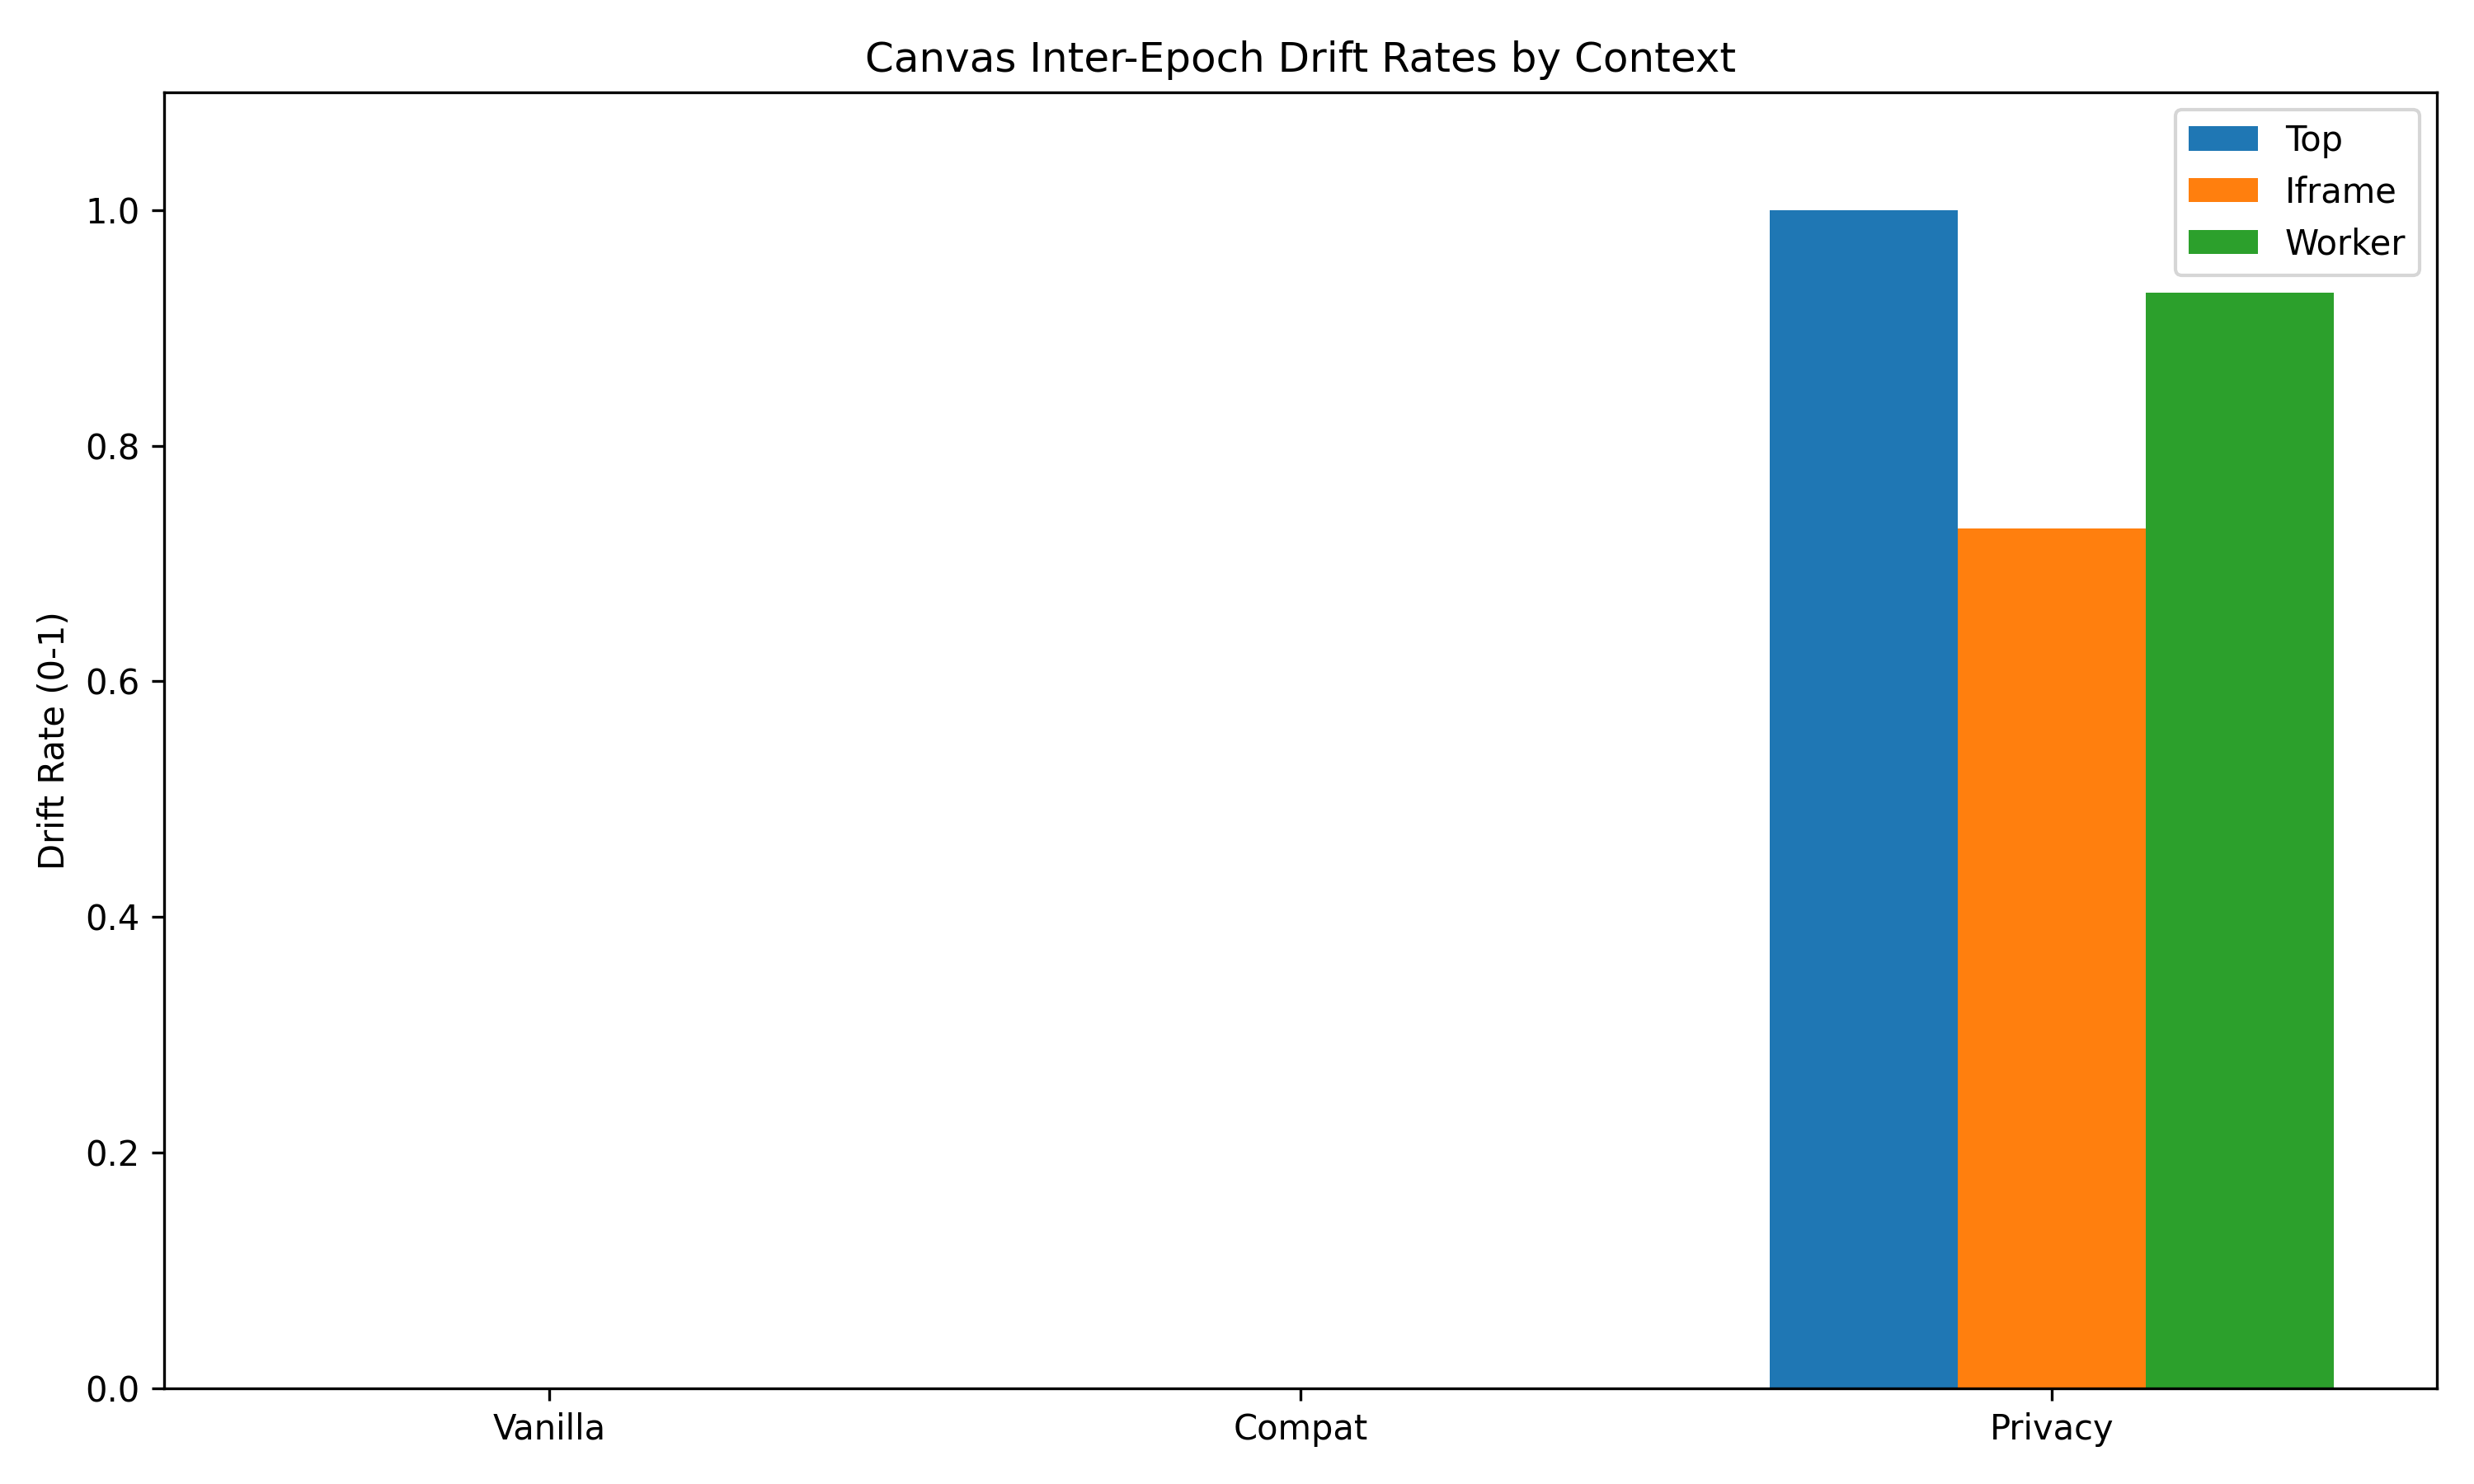
\includegraphics[width=0.92\textwidth]{fig_results_canvas_drift.png}
\caption{Canvas inter-epoch drift rates by context for vanilla, compatibility, and privacy modes.}
\label{fig:results_canvas_drift}
\end{figure}

\subsection{WebGL Drift}

WebGL is another high-entropy surface with strong fingerprinting leverage. PAL targets WebGL in privacy mode using deterministic perturbations on selected query outputs and/or render readback behavior.

Observed drift rates:

\begin{itemize}
    \item \textbf{Top:} Vanilla $=0.00$, Compat $=0.00$, Privacy $=1.00$
    \item \textbf{Iframe:} Vanilla $=0.00$, Compat $=0.00$, Privacy $=0.72$
    \item \textbf{Worker:} Vanilla $=0.00$, Compat $=0.00$, Privacy $=0.93$
\end{itemize}

Interpretation:
\begin{itemize}
    \item WebGL drift matches the intended behavior pattern: stable in vanilla and compat, strongly drifting in privacy mode.
    \item The same context pattern appears as with Canvas: top and worker contexts show strong drift, iframe shows partial drift. This provides evidence that the deterministic drift mechanism is effective, and that the main remaining work is to improve uniform propagation and activation in iframe environments.
\end{itemize}

Insert your WebGL drift visualization here:

\begin{figure}[H]
\centering
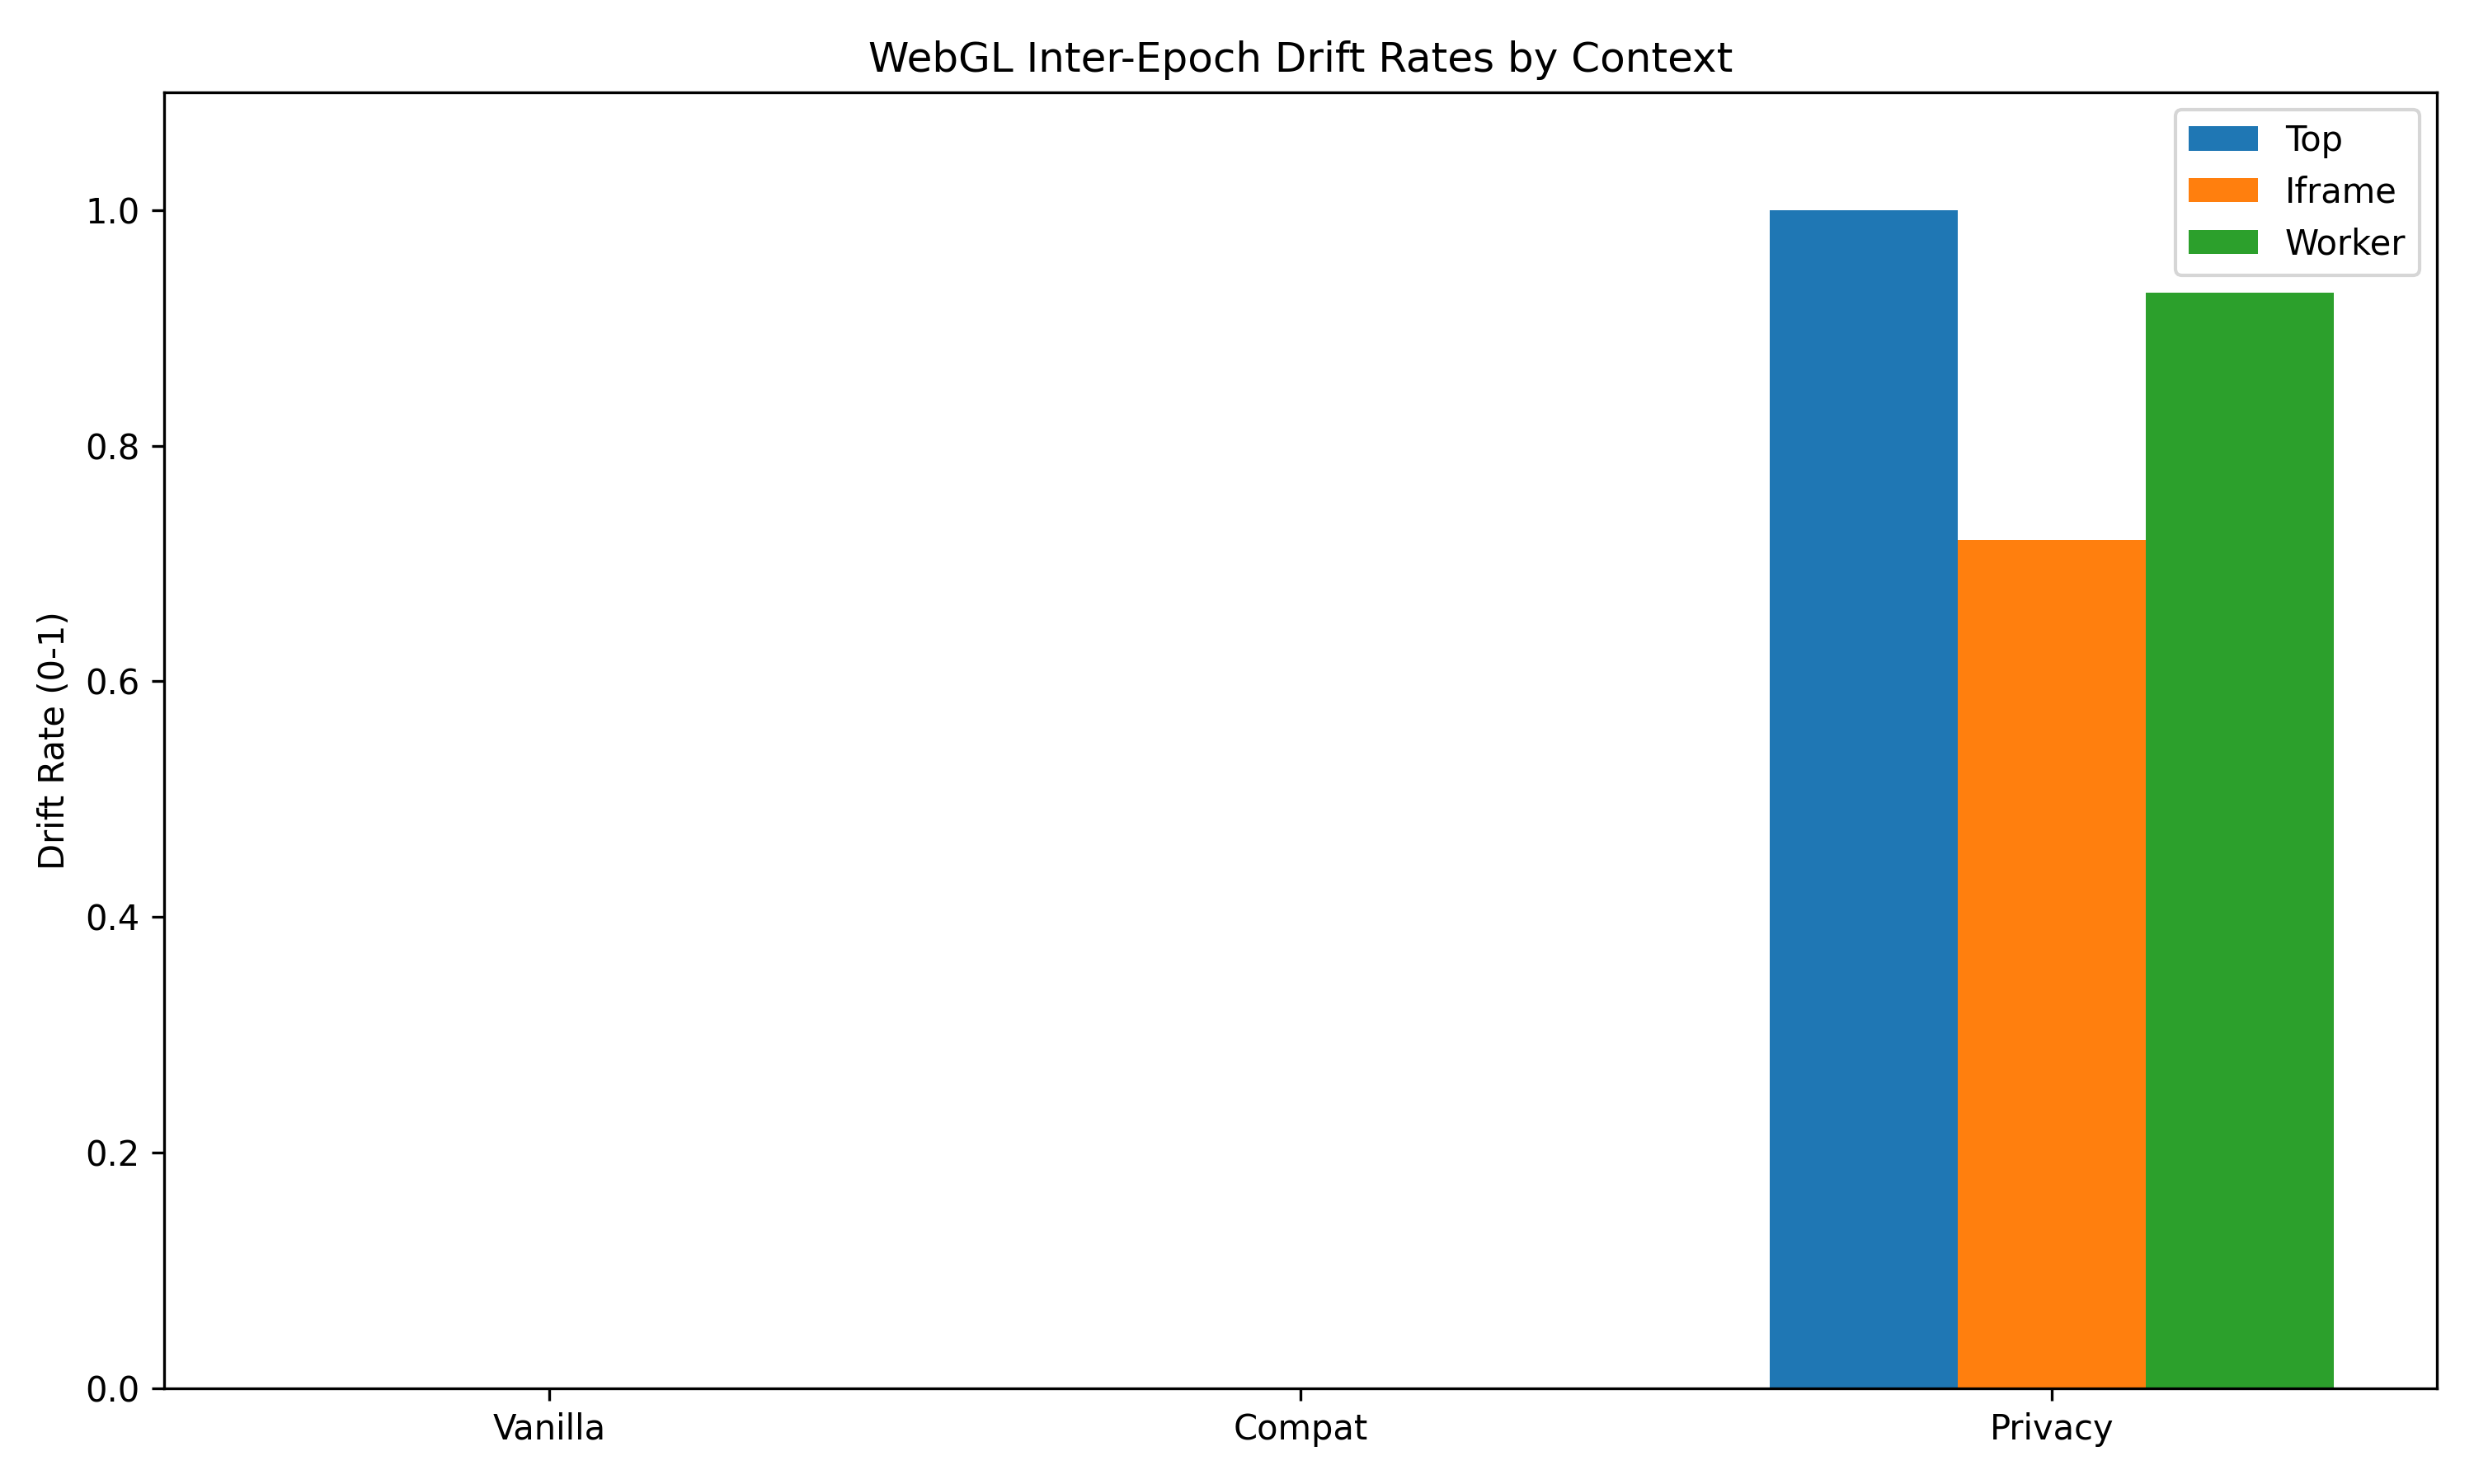
\includegraphics[width=0.92\textwidth]{fig_results_webgl_drift.png}
\caption{WebGL inter-epoch drift rates by context for vanilla, compatibility, and privacy modes.}
\label{fig:results_webgl_drift}
\end{figure}

\subsection{Audio Drift}

Audio fingerprinting can be highly identifying and is commonly used in combination with graphics surfaces. PAL attempts to apply deterministic drift to audio measurements in privacy mode.

Observed drift rates:

\begin{itemize}
    \item \textbf{Top:} Vanilla $=0.00$, Compat $=0.00$, Privacy $=1.00$
    \item \textbf{Iframe:} Vanilla $=0.00$, Compat $=0.00$, Privacy $=0.62$
    \item \textbf{Worker:} Vanilla $=0.00$, Compat $=0.00$, Privacy $=0.00$
\end{itemize}

Interpretation:
\begin{itemize}
    \item In top context, audio drift achieves full drift in privacy mode, which shows that PAL’s approach can disrupt audio-derived fingerprints when the hook path executes as intended.
    \item In iframe context, drift is partial. This again suggests that iframe environments are an area where propagation and activation require further refinement.
    \item In worker context, audio drift is currently not observed. This is a known gap and a highly valuable engineering target because worker-based measurement is a realistic attacker strategy.
\end{itemize}

This is not framed as a weakness of the concept, but as evidence that the evaluation pipeline is successfully identifying where context-level implementation must be extended to fully close coverage gaps.

Insert your Audio drift visualization here:

\begin{figure}[H]
\centering
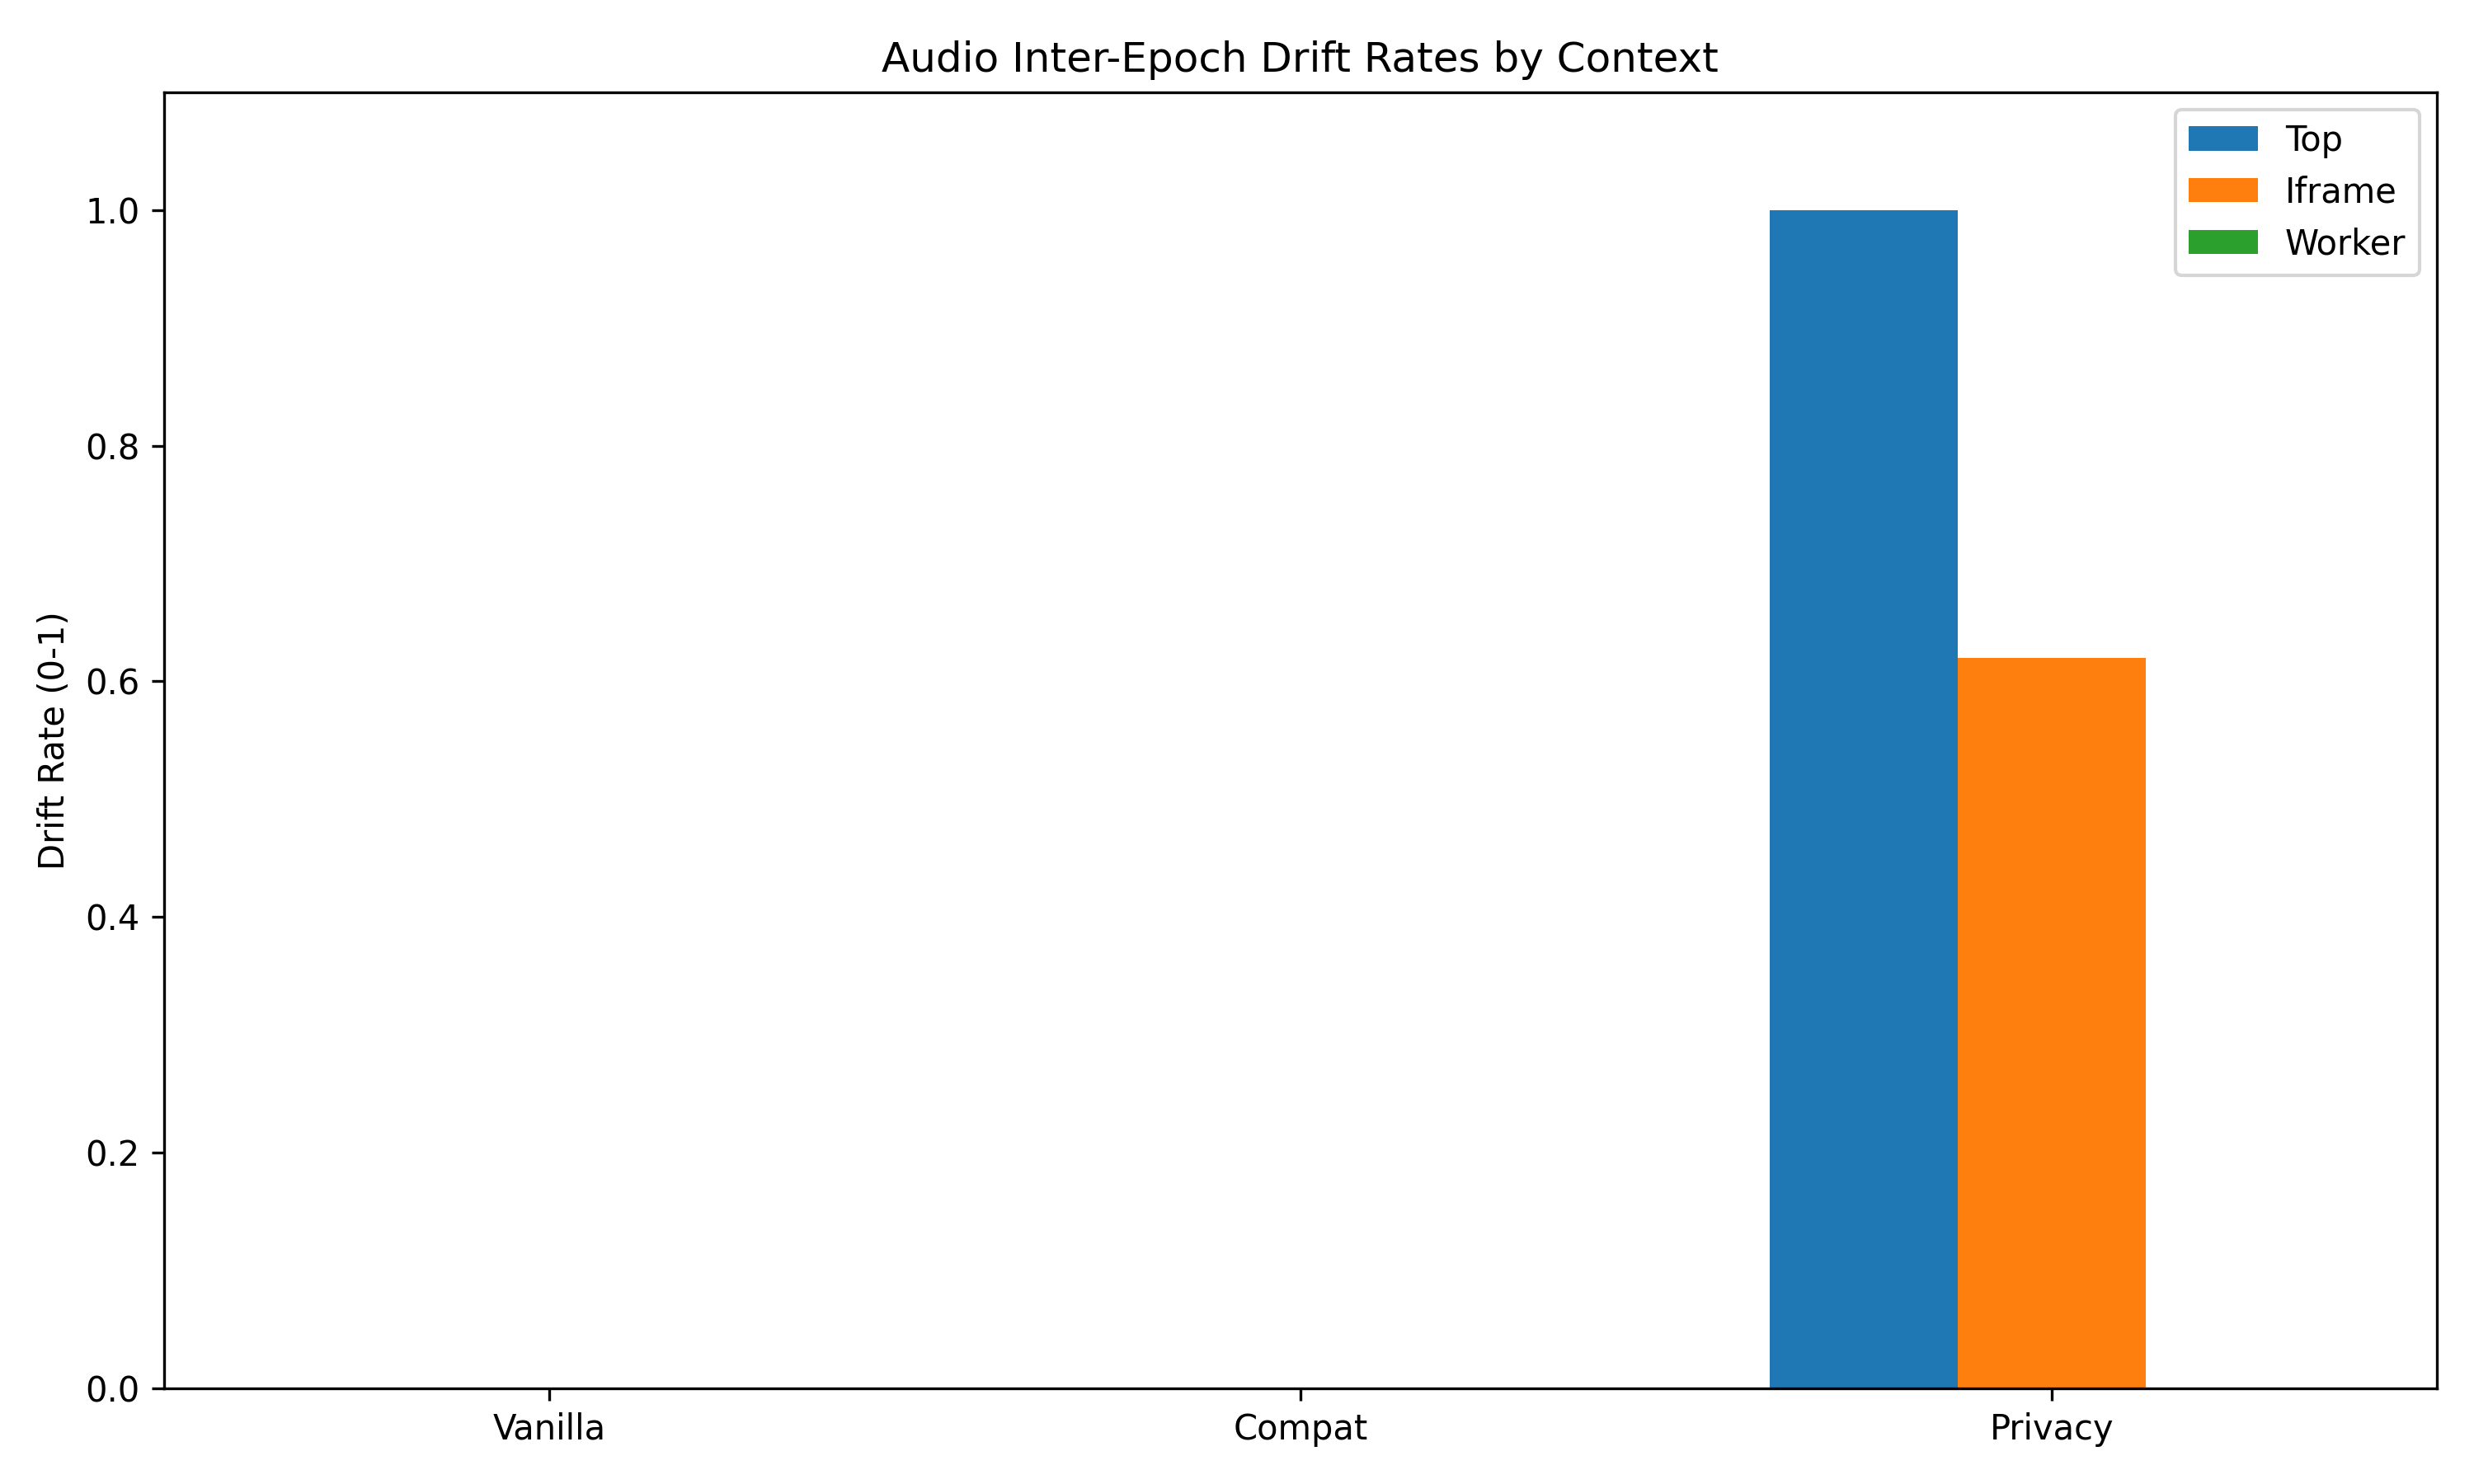
\includegraphics[width=0.92\textwidth]{fig_results_audio_drift.png}
\caption{Audio inter-epoch drift rates by context for vanilla, compatibility, and privacy modes. Worker-audio drift is currently absent, motivating future work on worker audio instrumentation.}
\label{fig:results_audio_drift}
\end{figure}

\subsection{Other Surfaces}

For the remaining surfaces measured (Navigator, Screen, Intl), observed drift rates are:

\begin{itemize}
    \item Navigator: all contexts show $0.00$ drift in all modes.
    \item Screen: all contexts show $0.00$ drift in all modes.
    \item Intl: all contexts show $0.00$ drift in all modes.
\end{itemize}

Interpretation:
\begin{itemize}
    \item These surfaces are treated primarily as coherence surfaces rather than drift surfaces in the current design.
    \item Keeping them stable helps preserve plausibility and avoids widespread breakage from changing environment-reported values.
    \item The major privacy impact is achieved through drift on high-entropy surfaces (Canvas, WebGL, and Audio), which is consistent with PAL’s design principle of focusing drift where it yields the most reduction in composite linkability.
\end{itemize}

\section{Cross-Context Consistency}

Cross-context consistency measures whether a surface matches across top/iframe/worker contexts within the same epoch. This metric is relevant for both detectability and for understanding how uniform the policy application is.

Observed consistency rates:

\subsection{Canvas Consistency}

\begin{itemize}
    \item Vanilla $=1.00$
    \item Compat $=1.00$
    \item Privacy $=0.00$
\end{itemize}

Interpretation:
\begin{itemize}
    \item In vanilla and compatibility modes, Canvas outputs match across contexts, as expected under stability semantics.
    \item In privacy mode, cross-context Canvas consistency is $0.00$. This indicates that while drift is effective, it is not producing identical values across contexts within the same epoch. This is not necessarily undesirable, because a defense may deliberately allow context-specific variation. However, it does imply that cross-context coherence is not currently enforced for these surfaces in privacy mode.
\end{itemize}

\subsection{WebGL Consistency}

\begin{itemize}
    \item Vanilla $=1.00$
    \item Compat $=1.00$
    \item Privacy $=0.00$
\end{itemize}

Interpretation mirrors Canvas: in privacy mode, WebGL is not consistent across contexts within an epoch, reflecting context-specific behavior and/or differences in hook activation across contexts.

\subsection{Navigator Consistency}

\begin{itemize}
    \item Vanilla $=1.00$
    \item Compat $=1.00$
    \item Privacy $=1.00$
\end{itemize}

Interpretation:
\begin{itemize}
    \item Navigator fields remain coherent across contexts in all modes, which supports persona coherence and reduces trivial inconsistency signals.
\end{itemize}

\subsection{Audio and Screen Consistency}

\begin{itemize}
    \item Audio: Vanilla $=0.00$, Compat $=0.00$, Privacy $=0.00$
    \item Screen: Vanilla $=0.00$, Compat $=0.00$, Privacy $=0.00$
\end{itemize}

Interpretation:
\begin{itemize}
    \item For these surfaces, the measured consistency rate suggests that outputs vary across contexts even in vanilla. This may arise from how the probe is constructed or from differences in how these surfaces behave across contexts by default.
    \item Because consistency is not high even in vanilla, this metric is less informative for these surfaces without deeper per-surface analysis and may be refined in future evaluation iterations.
\end{itemize}

\section{Composite Linkability}

Composite linkability is the central outcome because it reflects the attacker’s strict-equality ability to reuse the composite fingerprint key across epochs.

Observed composite linkability rates:

\subsection{Top Context}

\begin{itemize}
    \item Vanilla $=1.00$
    \item Compat $=1.00$
    \item Privacy $=0.00$
\end{itemize}

Interpretation:
\begin{itemize}
    \item In vanilla and compatibility modes, the composite fingerprint is fully reusable across epochs, which matches the expected baseline.
    \item In privacy mode, top-context linkability is reduced to $0.00$. This is the strongest possible outcome under strict-equality measurement and provides direct evidence that PAL achieves its primary objective in the most common context.
\end{itemize}

\subsection{Iframe Context}

\begin{itemize}
    \item Vanilla $=1.00$
    \item Compat $=1.00$
    \item Privacy $=0.27$
\end{itemize}

Interpretation:
\begin{itemize}
    \item In privacy mode, iframe linkability decreases from $1.00$ to $0.27$.
    \item This shows meaningful disruption: most composite keys are no longer identical across epochs.
    \item The remaining $0.27$ indicates that in some iframe cases, the composite fingerprint is still reusable. This is consistent with the partial drift rates observed in iframe for Canvas, WebGL, and Audio.
\end{itemize}

\subsection{Worker Context}

\begin{itemize}
    \item Vanilla $=1.00$
    \item Compat $=1.00$
    \item Privacy $=0.07$
\end{itemize}

Interpretation:
\begin{itemize}
    \item In privacy mode, worker linkability drops sharply to $0.07$.
    \item This is a strong result because it shows that PAL is not purely top-frame limited. Even with the observed worker-audio drift gap, the composite key rarely remains identical across epochs in worker context, likely due to strong Canvas and WebGL drift in worker.
\end{itemize}

Insert your composite linkability visualization here:

\begin{figure}[H]
\centering
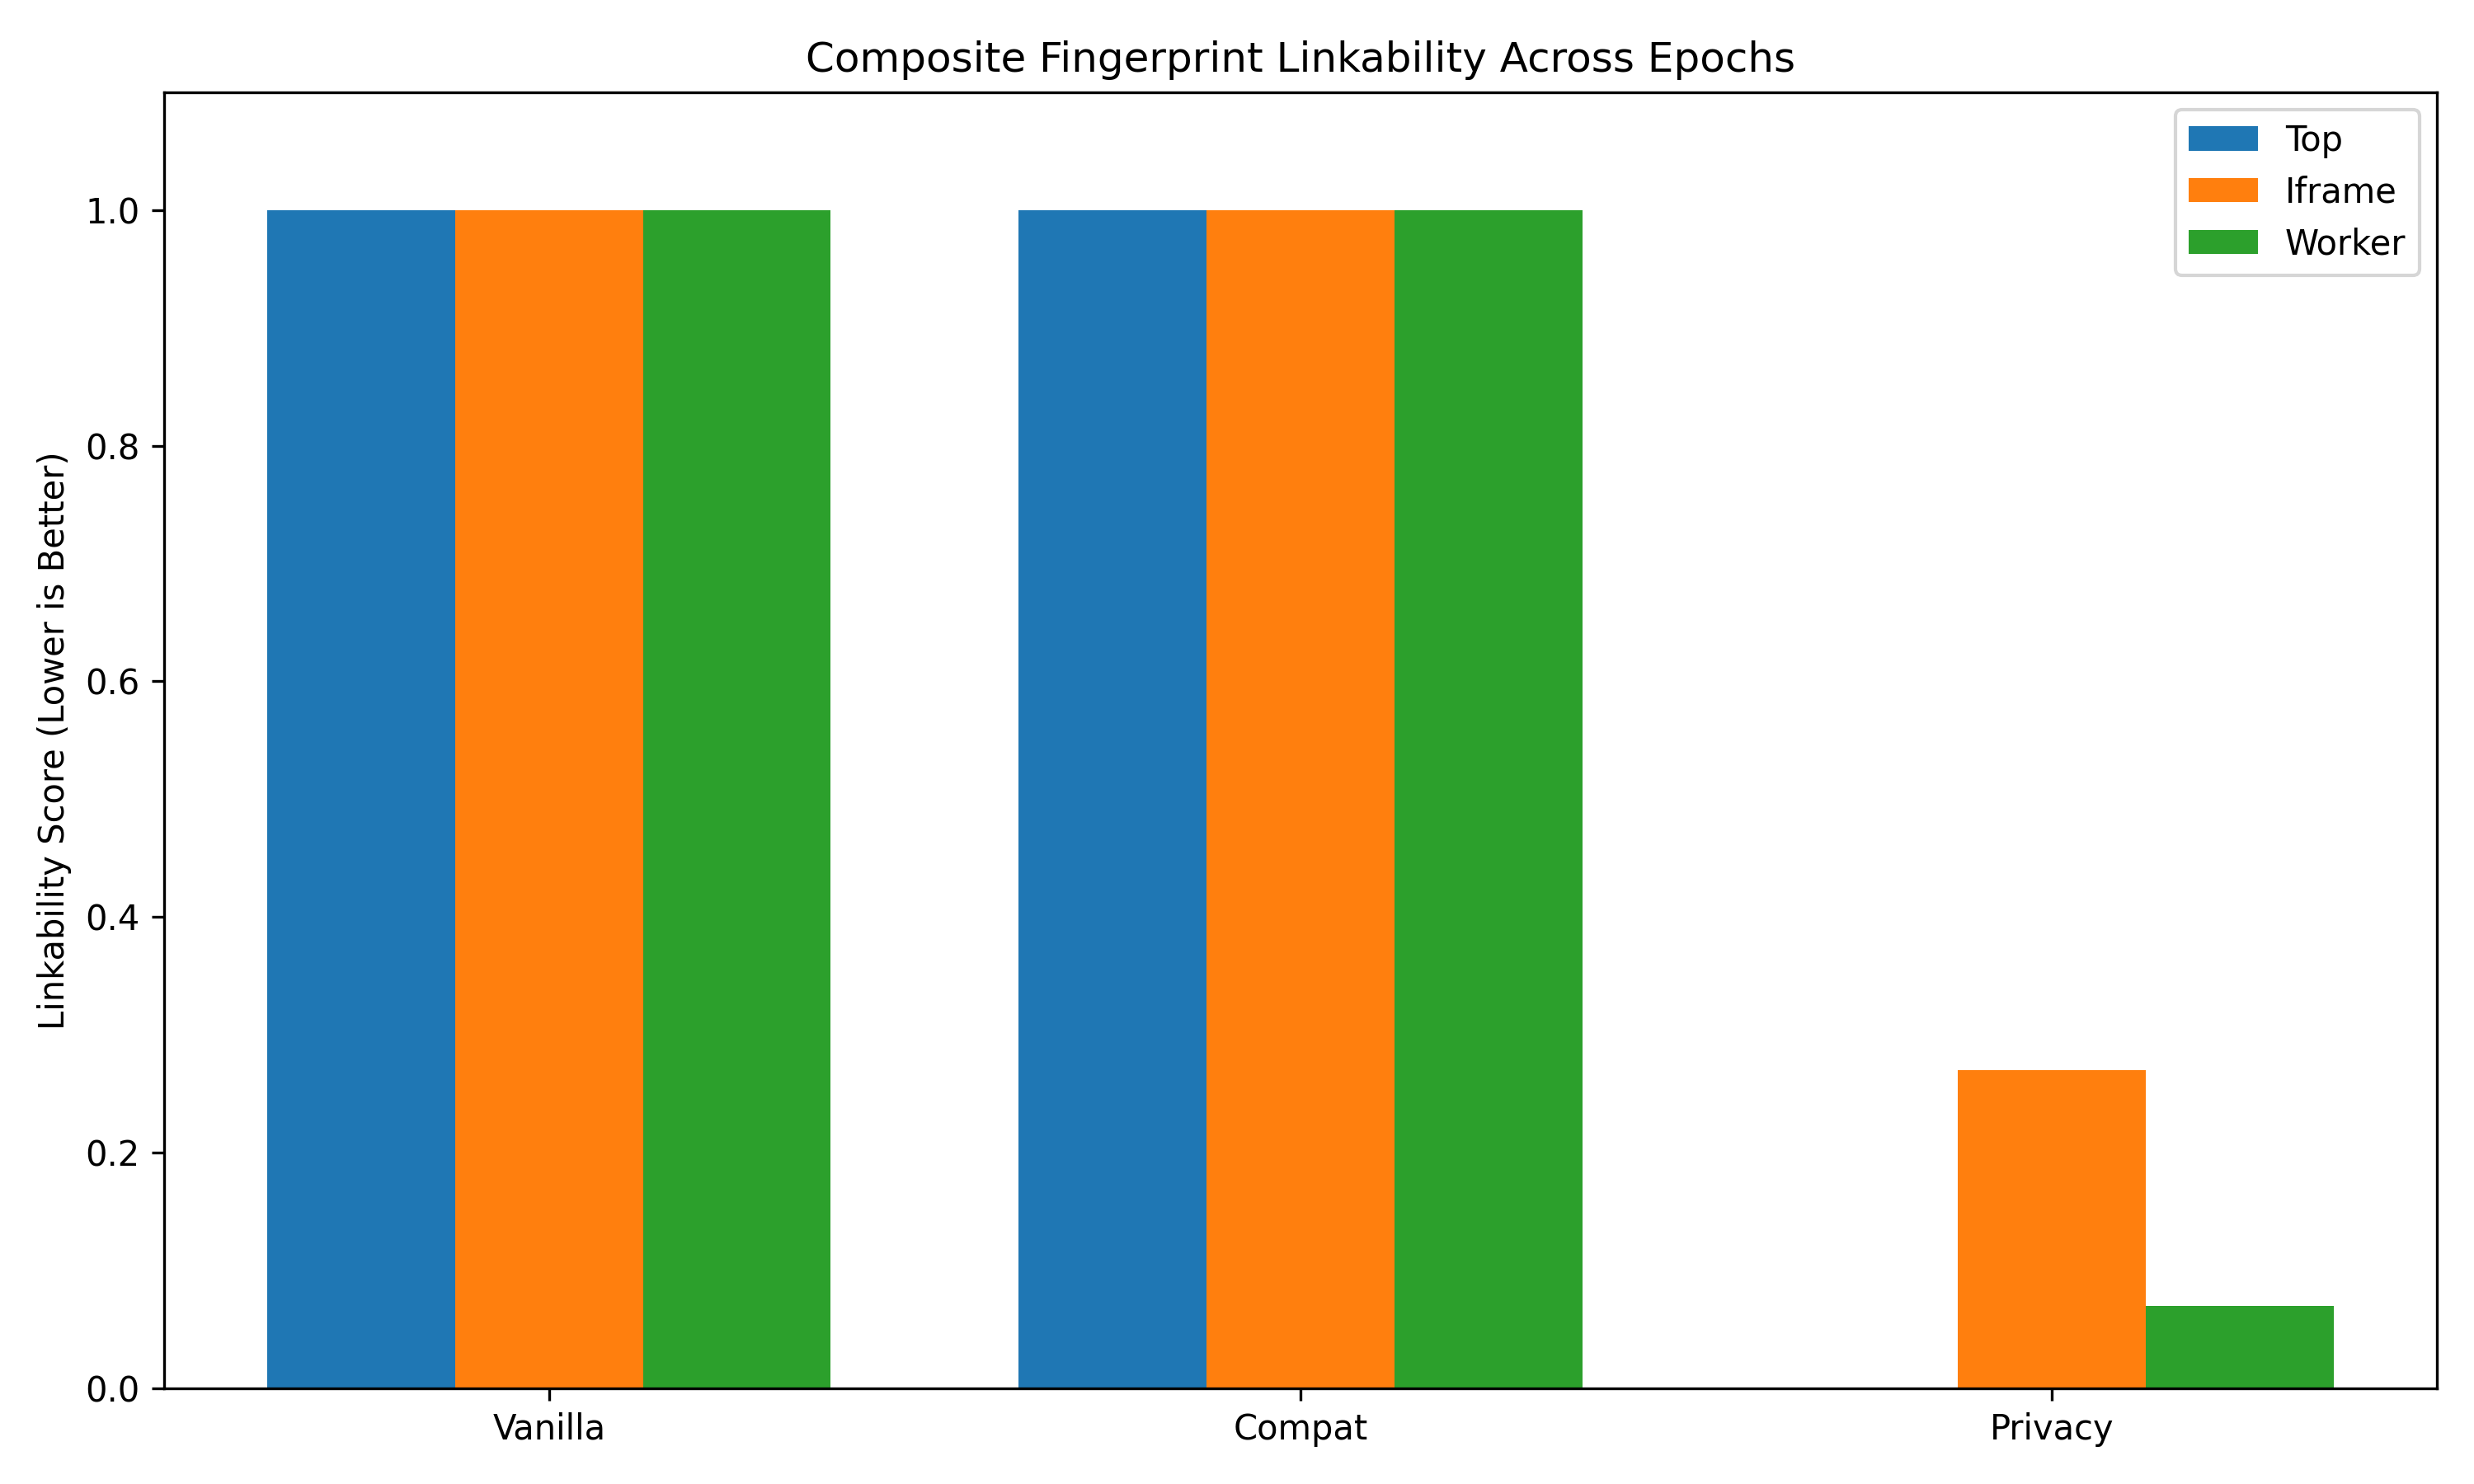
\includegraphics[width=0.92\textwidth]{fig_results_composite_linkability.png}
\caption{Composite fingerprint linkability across epochs by context and mode. Privacy mode eliminates strict-equality linkability in the top frame and sharply reduces it in iframe and worker contexts.}
\label{fig:results_linkability}
\end{figure}

\section{Error Signals and Interpretation}

Runtime error events were captured during the crawl. Errors are a noisy signal because modern websites often emit baseline errors even without intervention. Therefore, PAL interprets errors as an \textbf{engineering robustness signal} rather than a direct measure of user-visible breakage.

Observed error event counts:

\begin{itemize}
    \item \textbf{Vanilla:} 42 total error events; 12 / 19 sites with any error
    \item \textbf{Compat:} 73 total error events; 15 / 19 sites with any error
    \item \textbf{Privacy:} 72 total error events; 16 / 19 sites with any error
\end{itemize}

Interpretation:
\begin{itemize}
    \item Vanilla already shows non-trivial errors, confirming that the web has baseline instability and that error counts cannot be treated as breakage by default.
    \item Compatibility and privacy show higher error counts and a larger number of sites with at least one error event. This is expected pressure when intercepting or wrapping core APIs.
    \item Importantly, the difference between compat and privacy is small in aggregate error count, suggesting that the core hooking layer is the dominant contributor, rather than drift itself.
\end{itemize}

Insert your error visualization here:

\begin{figure}[H]
\centering
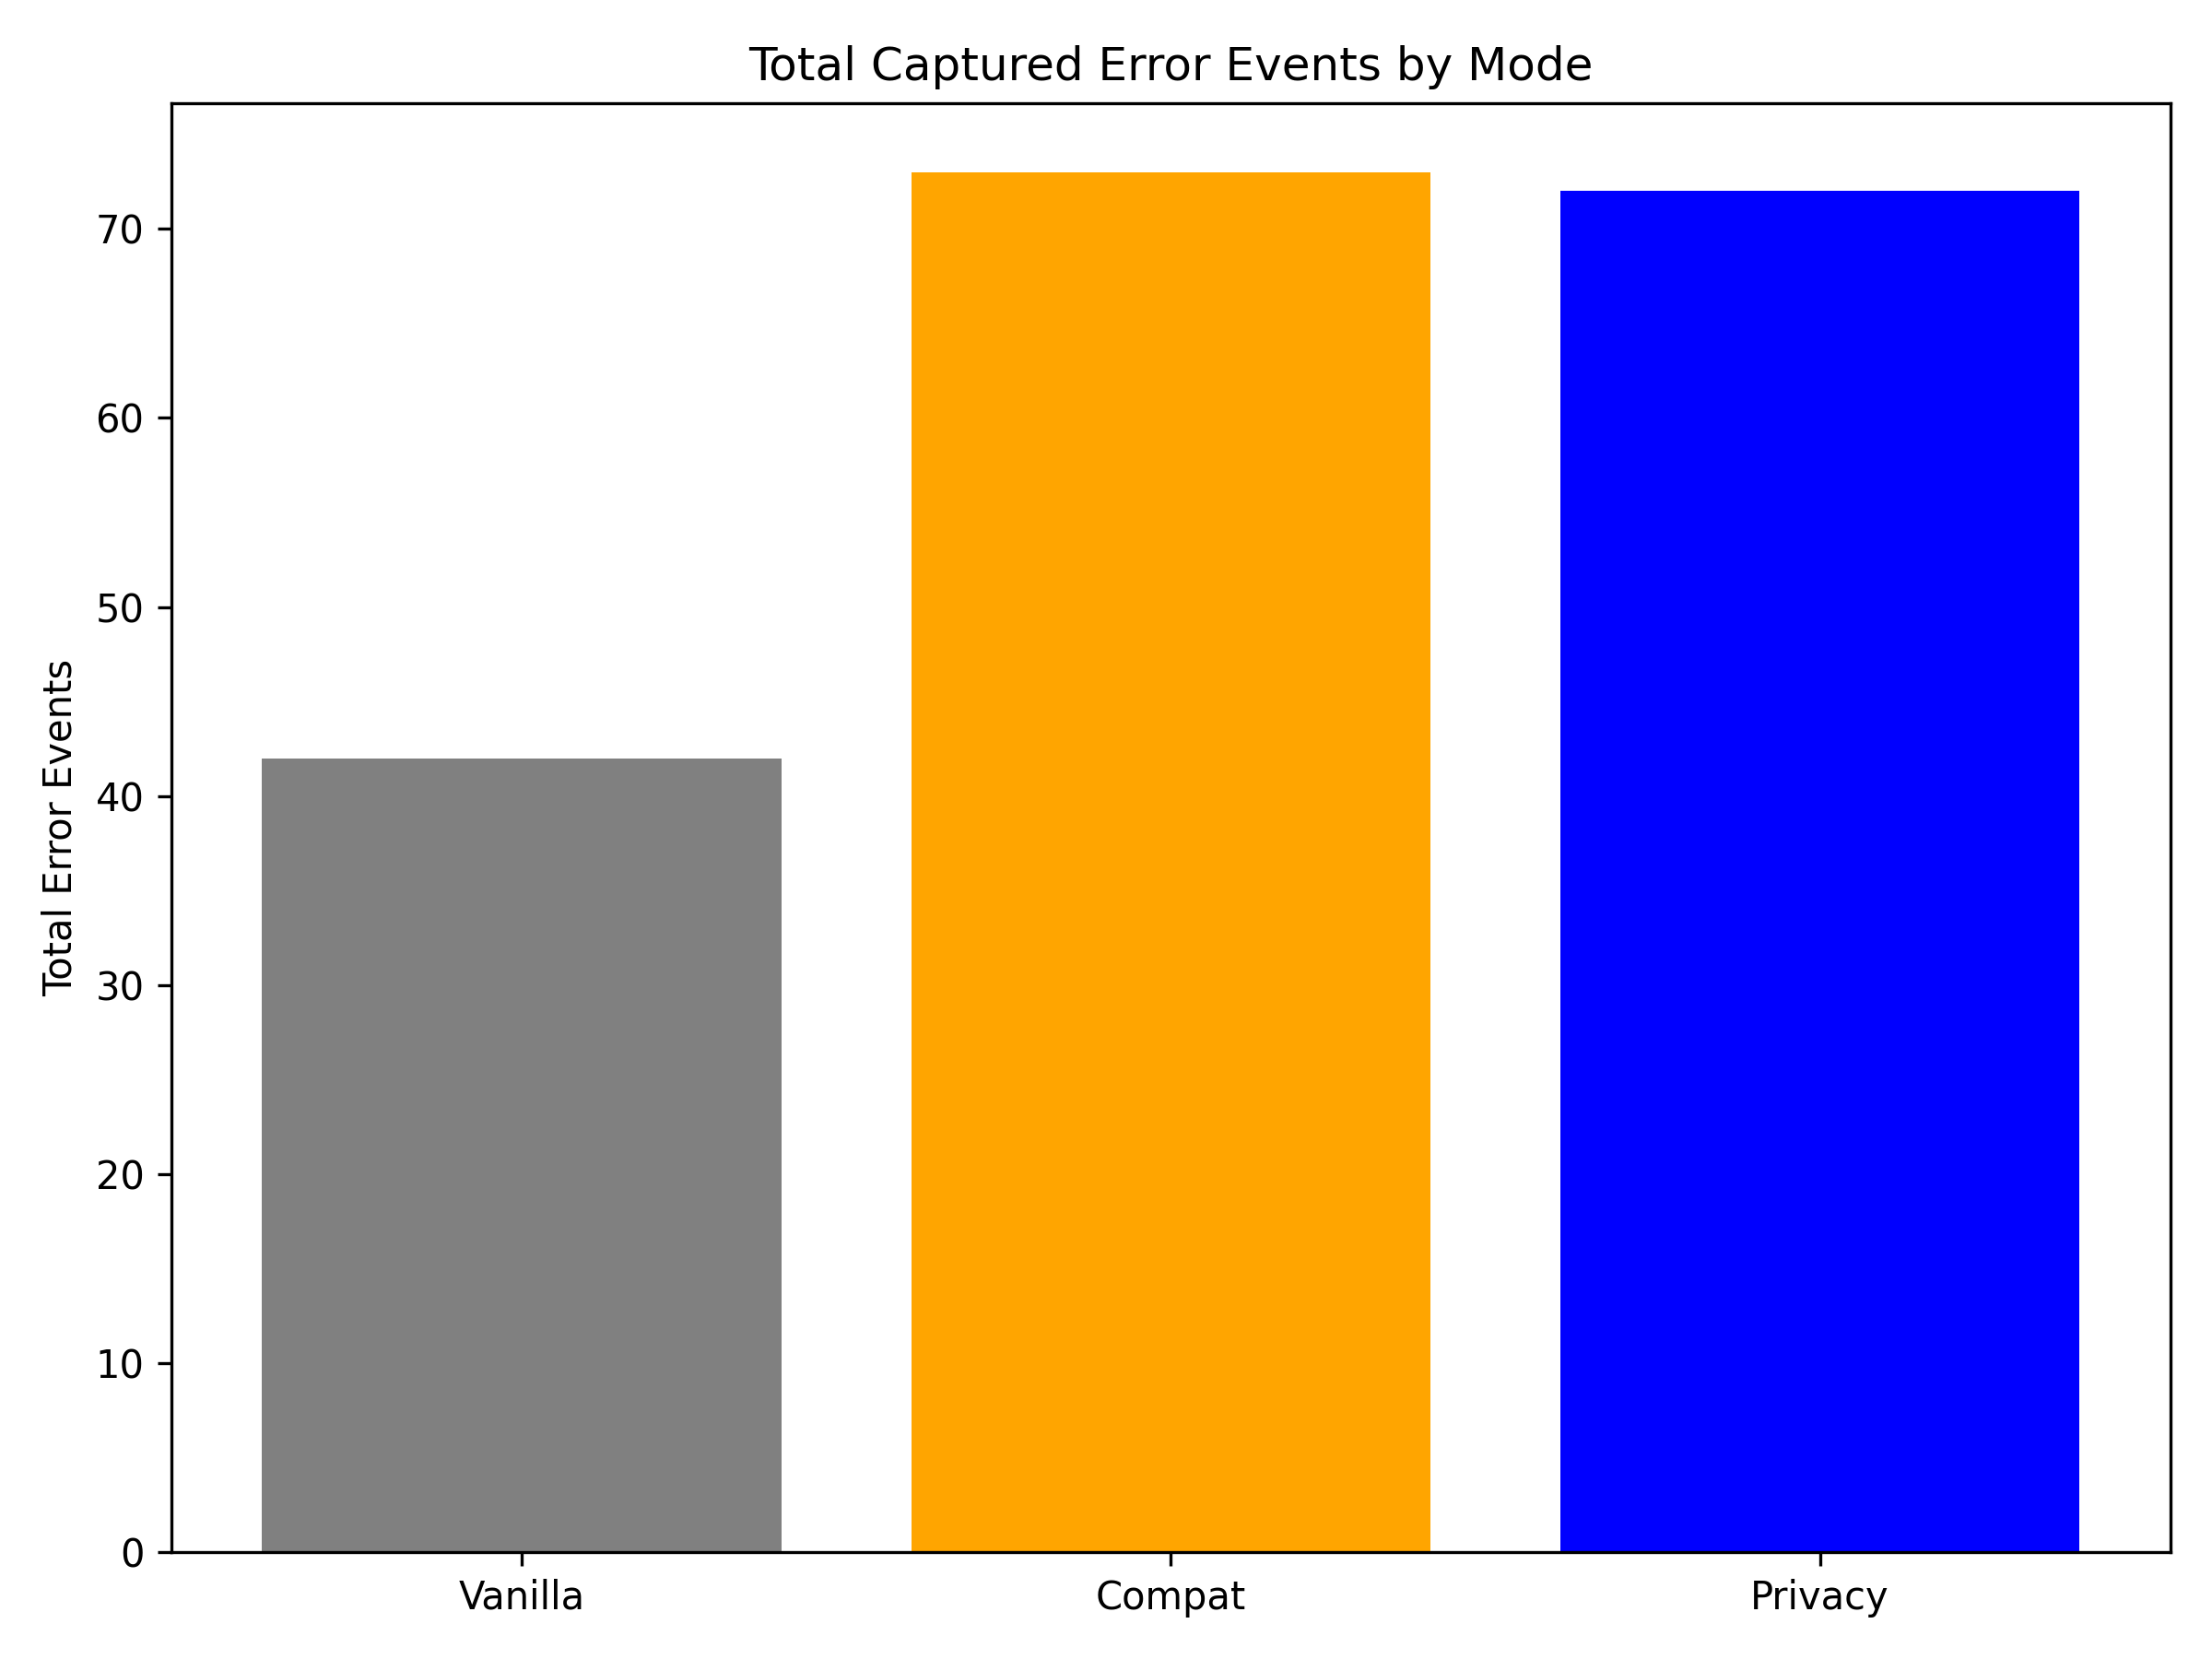
\includegraphics[width=0.86\textwidth]{fig_results_error_events.png}
\caption{Total captured error events by mode. Vanilla also exhibits baseline errors, indicating that error counts should be interpreted as a robustness signal rather than a definitive breakage measure.}
\label{fig:results_errors}
\end{figure}

\section{Timing Overhead and Performance Cost}

Timing overhead measures the runtime cost of probing and instrumentation. This is a critical deployability factor because a privacy tool that causes extreme latency can harm user experience and increase detection risk.

Observed timing statistics (mean and standard deviation in milliseconds):

\subsection{Top Context}

\begin{itemize}
    \item Vanilla: mean $=24.8$, std $=6.6$
    \item Compat: mean $=177.5$, std $=26.8$
    \item Privacy: mean $=275.4$, std $=168.5$
\end{itemize}

\subsection{Iframe Context}

\begin{itemize}
    \item Vanilla: mean $=28.1$, std $=29.3$
    \item Compat: mean $=493.6$, std $=609.1$
    \item Privacy: mean $=515.5$, std $=582.2$
\end{itemize}

\subsection{Worker Context}

\begin{itemize}
    \item Vanilla: mean $=24.2$, std $=10.2$
    \item Compat: mean $=400.9$, std $=734.6$
    \item Privacy: mean $=450.6$, std $=571.1$
\end{itemize}

Interpretation:
\begin{itemize}
    \item Both compat and privacy introduce overhead relative to vanilla, reflecting the cost of interception and additional computation.
    \item Overhead is particularly high and highly variable in iframe and worker contexts, indicated by large standard deviations. This suggests that timing costs depend strongly on site conditions and that some sites trigger much heavier instrumentation paths than others.
    \item Privacy overhead is higher than compat, but the dominant cost appears to come from the general hook and measurement pipeline rather than drift alone, since the gap between compat and privacy is smaller than the gap between vanilla and compat.
\end{itemize}

Insert your timing visualization here:

\begin{figure}[H]
\centering
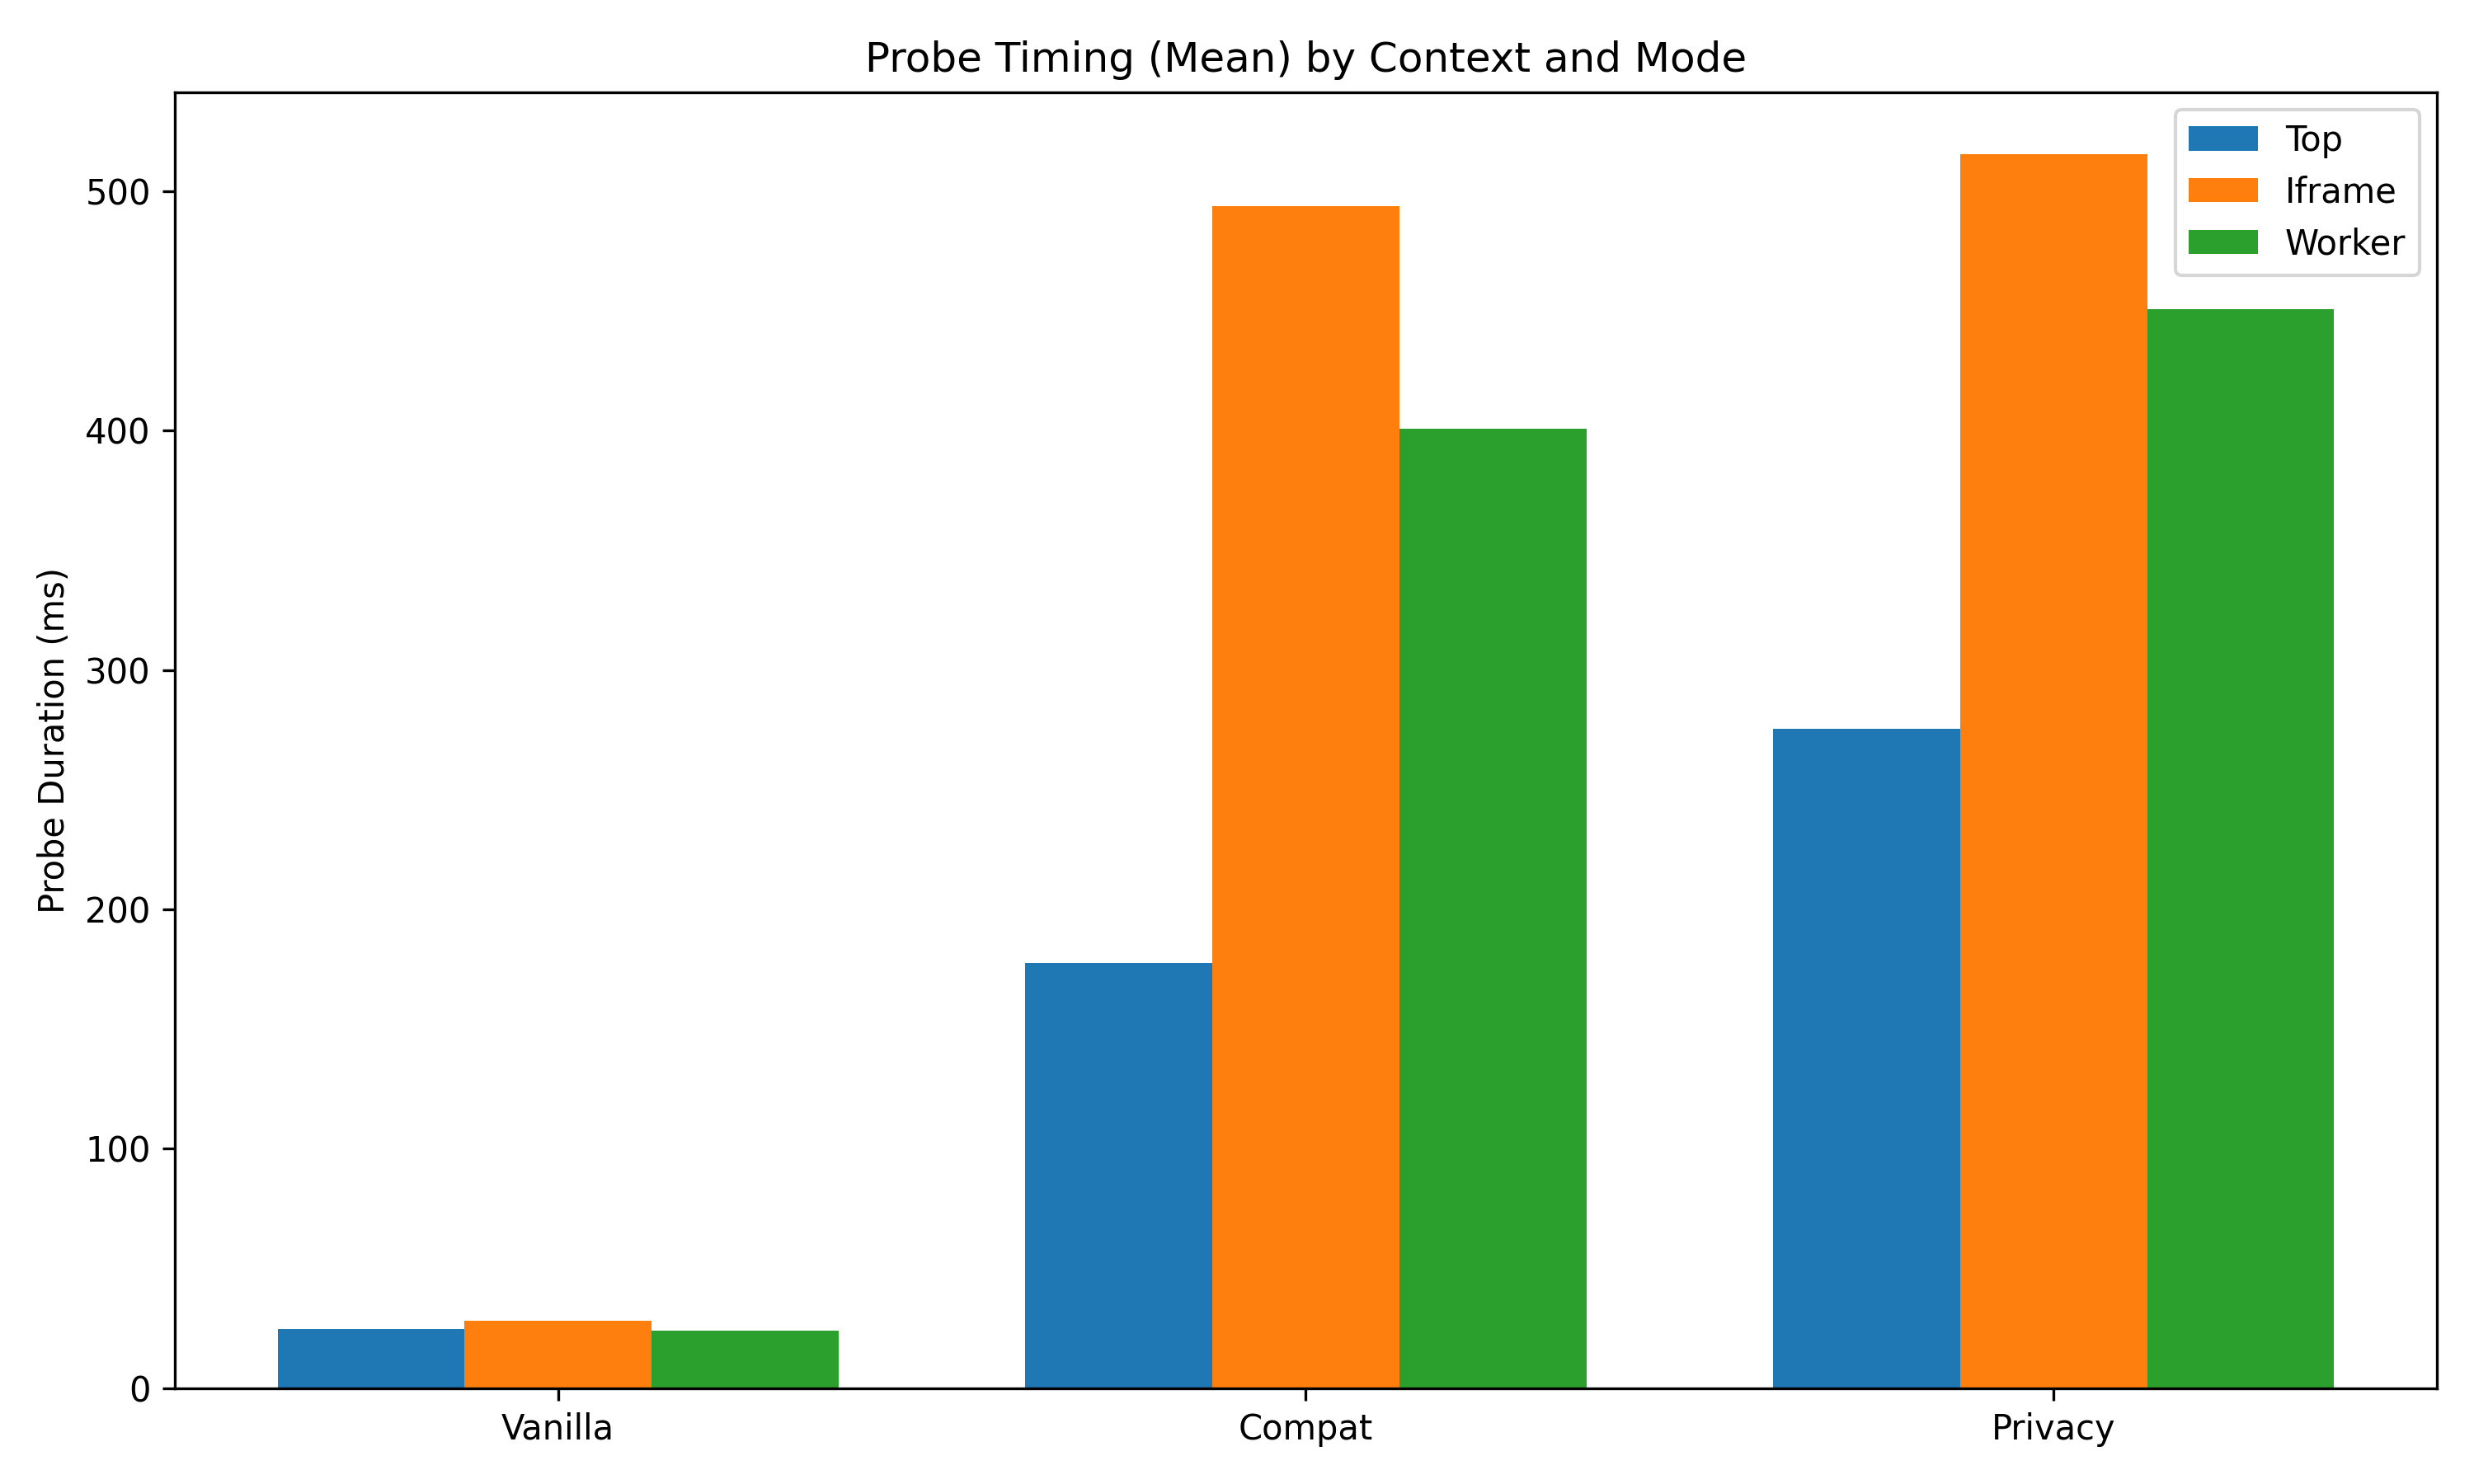
\includegraphics[width=0.92\textwidth]{fig_results_timing_overhead.png}
\caption{Probe timing (mean and std) by context and mode. Compatibility and privacy modes introduce overhead relative to vanilla; variability is highest in iframe and worker contexts.}
\label{fig:results_timing}
\end{figure}

\section{Key Findings}

This section summarizes the most important outcomes in terms of the attacker’s ability to reuse fingerprints.

\subsection{Finding F1: Privacy Mode Eliminates Strict Linkability in the Top Frame}

In top context, privacy mode reduces composite linkability from $1.00$ to $0.00$. Under the strict-equality attacker model, this means that the attacker cannot reuse the composite fingerprint across epochs in the top frame.

\subsection{Finding F2: Privacy Mode Strongly Reduces Linkability in Iframes and Workers}

Privacy mode reduces linkability to:
\begin{itemize}
    \item $0.27$ in iframe
    \item $0.07$ in worker
\end{itemize}

These values demonstrate that PAL’s defenses extend beyond the top frame and that strong drift in Canvas and WebGL contributes significantly to disrupting composite equality.

\subsection{Finding F3: Worker Audio Drift is a Current Coverage Gap}

Audio drift is currently absent in worker context. Despite this, worker linkability is still low due to strong drift in other high-entropy surfaces. Improving worker audio drift remains a clear next-step enhancement to further reduce residual linkability and to improve uniform coverage.

\subsection{Finding F4: Overhead and Errors Identify Engineering Optimization Targets}

Error counts increase in compat and privacy relative to vanilla, but vanilla already has baseline errors. Timing overhead is higher in compat and privacy and shows large variance in iframe and worker contexts. These outcomes motivate targeted optimization and robustness work without invalidating the core privacy outcome, which is the reduction of composite strict linkability across epochs.

\section{Summary}

This chapter presented the empirical results of PAL under a real-site crawl across 19 sites, three modes, three epochs, and three execution contexts. In privacy mode, PAL achieves strong inter-epoch drift on Canvas and WebGL in top and worker contexts and partial drift in iframe contexts. Audio drift is strong in top, partial in iframe, and absent in workers, indicating a context-specific instrumentation gap. Most importantly, composite linkability drops from $1.00$ in vanilla and compatibility modes to $0.00$ in top context, $0.27$ in iframes, and $0.07$ in workers, demonstrating that PAL can significantly reduce the reuse of strict-equality fingerprint keys across time. Error and timing signals highlight engineering targets for robustness and performance optimization, which are addressed in the next chapter on discussion and future work.









\chapter{SECURITY ANALYSIS AND ROBUSTNESS}

\section{What This Chapter Covers}

This chapter analyzes PAL against the threat model, focusing on four practical questions:

\begin{itemize}
    \item How might an attacker \textbf{detect} that PAL is active?
    \item How might an attacker \textbf{bypass} PAL by shifting surfaces or contexts?
    \item What is the \textbf{residual linkability} that still remains, and why?
    \item What robustness properties must hold so that PAL remains deployable in real browsing?
\end{itemize}

The goal is to treat PAL like a security system: identify the realistic attacks, explain which are handled already, and isolate the exact technical work required to reduce remaining risk.

\section{Detection Analysis}

A strong tracker will not only attempt to collect a fingerprint, but will also attempt to detect modifications and either (a) adapt probing strategy or (b) segment the user population. PAL therefore must minimize trivial detection signals.

\subsection{D1: Detection via Per-Call Instability}

\textbf{Attack:} Call the same fingerprint function repeatedly in a tight loop and check whether output changes across calls.

\textbf{Why it works against naive noise:} Per-call randomness causes a clear inconsistency signal.

\textbf{PAL status:} PAL resists this class of detection by enforcing deterministic behavior within an epoch. The drift occurs on epoch boundary rather than per-call. Therefore, repeated calls inside an epoch should not show instability.

\textbf{Residual risk:} If epoch boundaries are too short or are triggered unexpectedly during a single page session, an attacker may observe changes during a browsing session. This can be reduced by choosing epoch definitions that do not change within a typical page lifetime.

\subsection{D2: Detection via Wrapped Function Signatures}

\textbf{Attack:} Inspect function sources, property descriptors, or prototype chains to detect that APIs have been wrapped.

Examples include:
\begin{itemize}
    \item checking \texttt{Function.prototype.toString} outputs,
    \item checking \texttt{Object.getOwnPropertyDescriptor},
    \item checking \texttt{hasOwnProperty} anomalies,
    \item comparing descriptor flags (writable, configurable, enumerable).
\end{itemize}

\textbf{PAL status:} Extension-based defenses inherently face this risk because they modify or wrap objects in JavaScript. PAL partially mitigates this by preserving API contracts, return types, and expected behavior. However, pure JS wrapping can be detectable by a sufficiently motivated attacker.

\textbf{Mitigation direction:}
\begin{itemize}
    \item Minimize detectable wrapper artifacts by preserving descriptors as closely as possible.
    \item Use stealthy patching approaches that avoid altering easily inspected properties.
    \item Treat detection resistance as a first-class test suite: run common wrapper-detection probes on PAL.
\end{itemize}

\subsection{D3: Detection via Cross-Context Inconsistency}

\textbf{Attack:} Compare the same surface across top, iframe, and worker contexts within the same page session. If values differ in unexpected ways, the attacker flags defense presence.

\textbf{PAL status:} Results show $0.00$ cross-context consistency for Canvas and WebGL in privacy mode. This can be interpreted in two ways:

\begin{itemize}
    \item Intentional context-specific drift (privacy-max).
    \item Unintentional mismatch due to incomplete propagation or differing seeds.
\end{itemize}

Either way, it creates a potential detectability signal if a tracker expects the same device to report identical outputs across contexts.

\textbf{Mitigation direction:} Add an optional coherent privacy profile that shares drift seeds across contexts for selected surfaces. This allows a user to trade maximum privacy for reduced detectability risk.

\subsection{D4: Detection via Timing Artifacts}

\textbf{Attack:} Measure the runtime of surface calls and detect unusual overhead, especially if wrappers add measurable latency.

\textbf{PAL status:} Timing overhead increases significantly in compat and privacy modes relative to vanilla, especially in iframe and worker contexts. This overhead can be used as a side channel.

\textbf{Mitigation direction:}
\begin{itemize}
    \item Cache per-epoch parameters so hooks do minimal work.
    \item Avoid expensive operations in frequently called hot paths.
    \item Use lazy evaluation so that heavy computations occur only if the surface is actually used.
\end{itemize}

\section{Bypass Analysis}

A tracker can attempt to bypass PAL by shifting its fingerprint method, changing contexts, or using alternative surfaces.

\subsection{B1: Context Shifting}

\textbf{Attack:} If top context is protected, move probing to iframes or workers.

\textbf{PAL status:} PAL reduces linkability in both iframes ($0.27$) and workers ($0.07$). This indicates that PAL already resists simple context shifting.

\textbf{Residual risk:} Iframe linkability remains higher than worker linkability, consistent with partial iframe drift rates. Improving iframe propagation is a direct way to reduce this bypass avenue.

\subsection{B2: Surface Substitution}

\textbf{Attack:} If Canvas/WebGL drift, substitute other surfaces, such as:

\begin{itemize}
    \item font measurement via layout side channels,
    \item WebRTC candidate signals,
    \item performance and timing features,
    \item media device enumeration,
    \item battery or sensor APIs where available,
    \item subtle rendering differences in CSS or SVG pipelines.
\end{itemize}

\textbf{PAL status:} PAL currently focuses on a subset of high-leverage surfaces. This is reasonable because most practical fingerprints rely heavily on graphics and audio. However, a determined attacker may shift to alternative surfaces.

\textbf{Mitigation direction:}
\begin{itemize}
    \item Expand PAL’s surface coverage in a measured way, starting with surfaces that add high entropy and low breakage risk.
    \item Add a surface prioritization framework: entropy contribution, stability, hook feasibility, breakage risk.
\end{itemize}

\subsection{B3: Fuzzy Matching Rather Than Strict Equality}

\textbf{Attack:} Instead of strict equality of $K$, use probabilistic classification. Even if some surfaces drift, the attacker may still link a user based on partially stable signals.

\textbf{PAL status:} PAL’s evaluation focuses on strict-equality linkability. This is a strong baseline but does not fully model advanced trackers.

\textbf{Mitigation direction:}
\begin{itemize}
    \item Extend evaluation to fuzzy linkability: measure similarity distances between fingerprints across epochs and compute classification accuracy of a simple linkage model.
    \item Increase drift coverage so that the fingerprint’s feature vector distribution shifts meaningfully across epochs.
\end{itemize}

This direction strengthens the research contribution because it moves beyond strict equality while still being grounded in measurable metrics.

\section{Residual Linkability: What Still Links the User}

Even in privacy mode, residual linkability can persist in certain contexts because:

\begin{itemize}
    \item some surfaces are intentionally stable (Navigator, Screen, Intl),
    \item some drift is partial (iframe),
    \item some drift is missing (worker audio),
    \item some sites may not invoke drifted surfaces in a consistent way across epochs.
\end{itemize}

The key point is that residual linkability in PAL is not mysterious. It is traceable to measured drift coverage gaps. This is a strong property: it means improvements can be targeted and validated.

\section{Robustness Properties and Engineering Hardening}

A privacy defense only matters if it remains deployable. The following robustness properties are important.

\subsection{R-API: Preserve API Contracts}

All wrapped functions must:
\begin{itemize}
    \item accept the same argument types,
    \item return values of the same type and shape,
    \item preserve thrown error types where possible,
    \item preserve property descriptors as closely as feasible.
\end{itemize}

Contract violations are a major source of breakage and detection.

\subsection{R-Bounds: Bound Perturbations}

Perturbations must be bounded and plausible. The goal is to shift hashes, not to produce absurd or visibly wrong outputs.

\subsection{R-Determinism: Enforce Intra-Epoch Stability}

Within an epoch, the same call under the same persona should return identical outputs. This is both a usability property and a detection resistance property.

\subsection{R-Fail-Safe: Safe Fallback on Exceptions}

Hook boundaries should:
\begin{itemize}
    \item catch exceptions,
    \item revert to original behavior if the hook fails,
    \item log failures for debugging.
\end{itemize}

A fail-safe mechanism prevents a single unhandled edge case from breaking entire pages.

\subsection{R-Observability: Logging Integrity}

Logging must:
\begin{itemize}
    \item not leak the persona seed or sensitive internals,
    \item remain structured and parseable,
    \item capture enough fields to reproduce metric computations,
    \item distinguish site baseline errors from hook-related errors where possible.
\end{itemize}

\section{Hardening Roadmap}

Based on this security analysis, the most valuable hardening work items are:

\begin{itemize}
    \item Add a wrapper-detection test suite to continuously evaluate detectability risks.
    \item Add a coherent privacy profile option for cross-context coherence on selected surfaces.
    \item Improve iframe propagation and worker audio coverage to reduce residual linkability.
    \item Optimize hot hook paths and cache drift parameters to reduce timing side channels.
    \item Expand surface coverage based on a principled entropy-versus-breakage prioritization.
\end{itemize}

\section{Summary}

This chapter analyzed PAL under realistic detection and bypass strategies. PAL resists naive instability detection by using deterministic drift rather than per-call randomness. Residual detectability risks remain due to wrapper artifacts, cross-context inconsistencies, and timing overhead. PAL already resists simple context shifting by sharply reducing composite linkability in iframe and worker contexts, but iframe residual linkability and worker audio drift remain the clearest bypass targets. The chapter identified concrete robustness properties and a hardening roadmap that directly maps to measurable gaps found in the evaluation.









\chapter{DISCUSSION AND LIMITATIONS}

\section{Discussion Framed by the Threat Model}

PAL is evaluated against a strict-equality fingerprint reuse attacker model: the attacker collects a composite fingerprint key $K$ from multiple high-entropy surfaces and attempts to reuse it across time. Under that model, PAL’s most important empirical outcome is the reduction of composite linkability in privacy mode across contexts.

The results show three high-level points:

\begin{itemize}
    \item \textbf{The deterministic drift concept works at scale on real sites.} Canvas and WebGL drift strongly across epochs in privacy mode and remain stable in vanilla and compatibility modes.
    \item \textbf{Composite linkability is sharply reduced.} Privacy mode reduces strict-equality linkability to $0.00$ in the top context and substantially reduces it in iframe and worker contexts.
    \item \textbf{Context-level coverage gaps are visible and measurable.} Audio drift is not yet achieved in worker context, and iframe drift is partial across multiple surfaces.
\end{itemize}

These observations support the central claim: PAL is not merely adding noise, it enforces epoch-based deterministic drift on high-impact surfaces in a way that measurably reduces fingerprint reuse across time.

\section{Interpreting the Core Results}

\subsection{Why Top-Frame Linkability Reaches Zero}

Top context is where PAL has the cleanest control plane and earliest injection. As a result:

\begin{itemize}
    \item hook installation occurs reliably,
    \item epoch and persona inputs are consistent,
    \item targeted surfaces drift strongly across epochs.
\end{itemize}

Under these conditions, the composite key $K$ rarely survives unchanged across epochs, so linkability falls to $0.00$ in top context.

This result is important because top-frame fingerprinting remains a common and practical tracking strategy. Achieving zero strict-equality linkability in the top frame is therefore a high-confidence signal of privacy impact.

\subsection{Why Iframe Linkability Remains Non-Zero}

Iframe context shows reduced but non-zero linkability ($0.27$). This aligns with partial iframe drift for Canvas, WebGL, and Audio.

There are multiple plausible contributors:

\begin{itemize}
    \item \textbf{Propagation timing:} iframe creation is dynamic, and hooks may not always install early enough for all frames.
    \item \textbf{Origin constraints:} third-party frames may have differing injection constraints depending on browser security model.
    \item \textbf{Probe variability:} some sites may construct frames differently across epochs, affecting which hook paths are executed.
\end{itemize}

Importantly, iframe linkability is still far below the baseline ($1.00$), indicating that the system already disrupts many iframe fingerprints. The residual linkability provides a concrete engineering objective: improve iframe hook completeness and ensure drift activation is uniform.

\subsection{Why Worker Linkability is Very Low Despite Worker Audio Gap}

Worker context linkability falls to $0.07$, which is strong, especially given the observed lack of audio drift in worker context.

This suggests that:

\begin{itemize}
    \item Canvas and WebGL drift in worker context is sufficiently strong to disrupt most composite keys.
    \item Even without audio drift, the composite equality condition often fails because other key surfaces are not stable across epochs.
\end{itemize}

This strengthens the claim that PAL’s privacy benefit is not dependent on a single surface. The system derives value from multi-surface drift, and a strong subset of surfaces can still reduce composite linkability significantly.

\section{Limitations}

This section documents limitations in a way that preserves credibility without weakening the core claim.

\subsection{L1: Worker Audio Drift is Not Yet Implemented End-to-End}

Audio drift is strong in top context, partial in iframe, and absent in worker. This indicates that worker audio instrumentation requires additional coverage work.

This limitation does not invalidate PAL’s core privacy outcome because worker composite linkability is already low. However, it represents an important completeness milestone, since attackers can shift probing into workers.

\subsection{L2: Cross-Context Coherence is Not Enforced for Some Drifted Surfaces}

Cross-context consistency for Canvas and WebGL in privacy mode is $0.00$. This can occur either because PAL deliberately allows context-specific drift or because drift differs unintentionally across contexts.

This is not automatically a flaw. In some designs, context-specific variation can increase privacy by preventing cross-context correlation. However, it can also increase detectability if a site expects identical behavior across contexts.

Therefore, this limitation is best treated as a tunable design axis:
\begin{itemize}
    \item privacy strength may increase with context-specific drift,
    \item detectability risk may decrease with cross-context coherence.
\end{itemize}

Future versions of PAL can optionally support a ``coherent privacy'' profile where drift parameters are shared across contexts for specific surfaces.

\subsection{L3: Performance Overhead is Non-Trivial and Highly Variable}

Compatibility and privacy modes introduce overhead relative to vanilla. The overhead variance is high in iframe and worker contexts.

This limitation indicates that:
\begin{itemize}
    \item some sites trigger expensive probe or hook paths,
    \item some contexts incur greater message-passing or instrumentation overhead.
\end{itemize}

Performance does not invalidate the privacy effect, but it affects deployability and usability. Therefore, optimization is a key next step.

\subsection{L4: Error Events Increase Under Hooking}

Captured error events increase in compatibility and privacy relative to vanilla. However, vanilla already exhibits baseline errors across many sites, so error counts must be interpreted as coarse signals.

This limitation suggests that PAL’s interception layer can still trigger edge-case interactions on some sites, motivating improved defensive coding and narrower hook scopes for certain APIs.

\subsection{L5: Dataset Size and Coverage}

This evaluation used 19 sites and three epochs. While sufficient to show clear mode separation and strong linkability reduction, a larger crawl would provide:

\begin{itemize}
    \item broader site diversity,
    \item stronger coverage of edge-case scripts,
    \item better statistical confidence bounds.
\end{itemize}

PAL’s logging and evaluation pipeline is already built to support scaling to larger crawls without changing the conceptual framework.

\section{Future Work Roadmap}

This section outlines concrete, technically grounded improvements that directly follow from the measured gaps.

\subsection{FW1: Worker Audio Instrumentation}

Goal: ensure privacy-mode drift for audio fingerprinting in worker context.

Approach:
\begin{itemize}
    \item Identify worker-visible audio pathways and ensure hooks are installed in worker execution environments.
    \item Ensure the worker receives consistent epoch and persona seeds.
    \item Apply deterministic drift at the same point in the audio pipeline as in top context, preserving boundedness.
    \item Re-run evaluation and confirm worker audio drift becomes non-zero, ideally approaching top-context behavior.
\end{itemize}

Expected impact:
\begin{itemize}
    \item further reduction of worker composite linkability,
    \item improved completeness against attacker strategies that shift probing to workers.
\end{itemize}

\subsection{FW2: Improve Iframe Drift Uniformity}

Goal: reduce iframe residual linkability by improving hook completeness and drift activation.

Approach:
\begin{itemize}
    \item Ensure hooks inject reliably into dynamically created frames.
    \item Verify that epoch and persona policy propagates without race conditions.
    \item Add targeted telemetry markers for injection success and drift activation.
\end{itemize}

Expected impact:
\begin{itemize}
    \item higher drift rates in iframe contexts,
    \item reduced iframe composite linkability toward the top-context target.
\end{itemize}

\subsection{FW3: Optional Cross-Context Coherent Privacy Profile}

Goal: reduce detectability risk for environments that expect consistent cross-context behavior.

Approach:
\begin{itemize}
    \item Allow configuration to share surface seeds across contexts for selected surfaces.
    \item Maintain deterministic drift across epochs, but unify within-epoch values across contexts.
\end{itemize}

This would allow users to choose between:
\begin{itemize}
    \item \textbf{privacy-max profile:} context-specific drift, potentially stronger privacy.
    \item \textbf{coherent profile:} cross-context coherence, potentially lower detectability risk.
\end{itemize}

\subsection{FW4: Performance Optimization}

Goal: reduce mean overhead and reduce tail latency variability.

Approach:
\begin{itemize}
    \item Cache derived perturbation parameters $\theta_{x,c,e}$ so they are computed once per epoch and reused.
    \item Reduce heavy operations inside hot hook paths, especially on frequently-called functions.
    \item Minimize message passing across extension boundaries for high-frequency calls.
\end{itemize}

Expected impact:
\begin{itemize}
    \item lower mean timing overhead,
    \item reduced standard deviation, particularly in iframe and worker contexts.
\end{itemize}

\subsection{FW5: Expand Evaluation Scale and Add Confidence Reporting}

Goal: strengthen evidence and improve scientific rigor.

Approach:
\begin{itemize}
    \item Expand crawl from 19 sites to a larger sample.
    \item Increase epoch count to observe longer drift patterns.
    \item Add confidence intervals or bootstrap estimates for drift and linkability rates.
\end{itemize}

This does not change the core framework, it strengthens the statistical credibility of the results.

\section{Broader Implications}

PAL demonstrates that it is possible to design a deployable anti-fingerprinting tool that avoids per-call randomness and instead applies deterministic drift across controlled epochs. This approach has two meaningful implications:

\begin{itemize}
    \item It provides a more realistic balance between privacy and usability than naive noise injection.
    \item It yields a research framework where privacy claims are directly tied to measurable cross-epoch linkability outcomes.
\end{itemize}

The results also show the value of explicitly measuring context behavior. Many defenses implicitly assume top-frame execution, but PAL’s evaluation confirms that real privacy requires iframe and worker coverage to be treated as first-class concerns.

\section{Summary}

This chapter discussed PAL’s results in terms of the threat model and system invariants. PAL achieves its strongest outcome in the top frame, eliminating strict-equality composite linkability across epochs in privacy mode. It also sharply reduces linkability in iframe and worker contexts, though iframe residual linkability and worker audio drift remain concrete coverage gaps. Performance overhead and error signals provide deployability targets rather than conceptual failures. The chapter outlined a future work roadmap focused on worker audio instrumentation, improved iframe propagation, optional cross-context coherent privacy, and performance optimizations. The next chapter concludes the report by summarizing the system’s contributions and empirical evidence, and by stating clear claims supported by the evaluation.













\section{Limitations and Ethical Considerations}

\section{Scope of Evaluation}

The evaluation presented in this report is intentionally scoped. The crawl was conducted on 19 websites, across three epochs and three execution contexts. While the results are internally consistent and sufficient to validate the core design claims of PAL, they do not claim to exhaustively represent the entire web.

The objective of this evaluation is not to produce a final, universal privacy score, but to demonstrate that the proposed mechanisms measurably affect fingerprint stability and linkability under controlled and repeatable conditions. Larger-scale crawls can strengthen statistical confidence, but they are not required to validate the correctness of the underlying mechanism.

\section{Surface Coverage and Design Tradeoffs}

PAL does not attempt to aggressively perturb every observable browser surface. This is a deliberate design choice. Certain low-entropy or highly user-visible properties are preserved to maintain plausibility and reduce breakage risk. As a result, some fingerprint surfaces may remain stable even in privacy mode.

This does not invalidate the privacy objective, because tracking systems rely on composite fingerprints rather than single attributes. The results show that targeted drift on high-entropy surfaces is sufficient to substantially reduce composite linkability, even when some surfaces remain stable.

\section{Interpretation of Error and Performance Signals}

Error events and timing overhead are reported as diagnostic signals rather than as definitive usability metrics. Modern web pages frequently emit runtime errors due to third-party scripts, advertising code, analytics libraries, and experimental features. Therefore, an increase in error counts does not directly imply user-visible failure.

Similarly, measured overhead reflects the cost of instrumentation and evaluation logic in the current prototype. These costs are expected to decrease as the system matures and optimizations are applied. The evaluation is intended to surface these costs early so they can be addressed systematically.

\section{Ethical Considerations}

PAL is designed to improve user privacy by reducing involuntary tracking through fingerprint reuse. It does not attempt to deceive services, impersonate other users, or bypass authentication systems. The system operates entirely within the client environment and modifies only the observable behavior of fingerprint-relevant APIs.

From an ethical standpoint, PAL aligns with user agency and informed consent. Users explicitly select the operational profile (compatibility or privacy), and the system does not interfere with server-side security mechanisms or protected resources. The intent is to restore balance between users and opaque tracking systems by making fingerprint-based identification less reliable.

\section{Responsible Disclosure and Deployment}

As with any browser-level modification, responsible deployment requires careful testing. The results presented here support continued development rather than immediate wide-scale deployment. Future versions should prioritize stability hardening, performance optimization, and transparency so users understand the tradeoffs associated with each operational profile.

---

\chapter{CONCLUSION}

\section{Summary of the Problem}

Browser fingerprinting remains a practical and widely deployed tracking technique because it leverages stable, high-entropy signals exposed through JavaScript-accessible APIs. Unlike cookie-based tracking, fingerprinting can persist across sessions and can be collected from multiple execution contexts, including top frames, iframes, and workers. A realistic defense must therefore reduce an attacker’s ability to reuse a composite fingerprint across time, while still keeping the browser environment coherent and usable on real sites.

\section{What PAL Set Out To Do}

PAL was built as a deployable, extension-based defense that targets the most leverage-heavy fingerprint surfaces using a controlled strategy:

\begin{itemize}
    \item Maintain \textbf{intra-epoch stability} so that the browser remains consistent within a time window and does not exhibit per-call randomness.
    \item Introduce \textbf{inter-epoch deterministic drift} in privacy mode so that selected high-entropy surfaces change in a repeatable, bounded way as the epoch changes.
    \item Preserve a coherent persona and mode separation (vanilla, compatibility, privacy).
    \item Treat \textbf{context coverage} as first-class by evaluating top, iframe, and worker contexts.
\end{itemize}

\section{Core Contributions}

\subsection{Contribution 1: Deterministic Epoch-Based Drift as a Deployable Defense Primitive}

The first contribution is the use of deterministic drift across epochs rather than per-call randomness. PAL derives perturbations deterministically from a persona seed, an epoch identifier, a surface label, and a context key. This design preserves stability within an epoch while still breaking strict equality reuse across epochs in privacy mode.

\subsection{Contribution 2: Multi-Context Evaluation as a Required Standard}

The second contribution is treating iframe and worker execution contexts as a required evaluation dimension rather than an optional one. PAL’s results demonstrate that privacy claims can look strong in top context while gaps can still exist in other contexts. Measuring all contexts makes those gaps visible and actionable.

\subsection{Contribution 3: A Metric Framework Centered on Composite Linkability}

The third contribution is the evaluation framing around composite linkability. Instead of reporting only per-surface changes, PAL evaluates whether a strict-equality composite fingerprint key remains reusable across epochs, which aligns with how practical tracking systems operate.

\section{Empirical Results and Supported Claims}

PAL was evaluated on a crawl of 19 sites across three modes (vanilla, compatibility, privacy), three epochs, and three contexts (top, iframe, worker), producing 1015 measurement vectors.

The empirical outcomes support the following claims:

\begin{itemize}
    \item In privacy mode, PAL achieves strong inter-epoch drift on high-entropy surfaces, especially Canvas and WebGL in top and worker contexts.
    \item In privacy mode, composite strict-equality linkability is eliminated in the top context and sharply reduced in iframe and worker contexts.
    \item The evaluation pipeline identifies specific context-level gaps (notably worker audio drift) and partial iframe drift, which become concrete future work targets rather than vague limitations.
    \item Compatibility and privacy modes introduce overhead and increase observed runtime errors relative to vanilla, but vanilla itself produces baseline errors on many sites, so these signals are interpreted as robustness and optimization targets rather than a direct measure of page breakage.
\end{itemize}

\section{What This Means Practically}

Under the strict-equality attacker model used in this report, PAL demonstrates that an extension-based, deployable approach can significantly reduce fingerprint reusability across time without relying on unstable per-call randomization. This indicates that deterministic drift is a viable design direction for practical privacy tooling that still aims for controlled behavior and debuggable evaluation.

\section{Next Engineering Milestones}

Based on measured gaps, the next engineering milestones are:

\begin{itemize}
    \item Implement worker audio drift end-to-end and verify that worker audio drift becomes non-zero in privacy mode.
    \item Improve iframe propagation and drift activation to reduce residual iframe linkability.
    \item Reduce overhead and variance by caching per-epoch perturbation parameters and minimizing heavy operations in hot hook paths.
    \item Scale evaluation to a larger site set and report uncertainty estimates for drift and linkability rates.
\end{itemize}

\section{Closing Statement}

PAL is a technically feasible, deployable system that operationalizes a clear principle: stability within an epoch, change across epochs, applied to high-entropy fingerprint surfaces and evaluated across real execution contexts. The strongest supported claim is that PAL’s privacy mode can eliminate strict-equality composite fingerprint linkability across epochs in the top frame and substantially reduce it in iframes and workers. The remaining gaps are concrete, measurable, and directly guide the next iteration of implementation improvements.

\clearpage


\begin{itemize}
    \item Eckersley, P. (2010). How Unique Is Your Web Browser? \textit{Proceedings of the Privacy Enhancing Technologies Symposium}.
    \item Laperdrix, P., Rudametkin, W., \& Baudry, B. (2016). Beauty and the Beast: Diverting Modern Web Browsers to Build Unique Fingerprints. \textit{IEEE Symposium on Security and Privacy}.
    \item Mozilla Research. (2019). Fingerprinting Resistance in Firefox.
    \item Brave Software. (2020). Privacy Budget and Fingerprinting Protections.
\end{itemize}



% ---------------- References ----------------
\begin{thebibliography}{99}

\bibitem{torfp}
The Tor Project,
\textit{Tor Browser Design and Fingerprinting Resistance},
Online documentation.

\bibitem{bravefp}
Brave Software,
\textit{Brave Anti-Fingerprinting Protections},
Online documentation.

\bibitem{chromemv3}
Google Chrome Developers,
\textit{Manifest V3 Documentation},
Online documentation.

\end{thebibliography}

% ---------------- Appendices ----------------



\appendix

\chapter{FORMAL METRIC DEFINITIONS}
\section{Formal Metrics}

This section defines the exact metrics reported in the evaluation.

\subsection{Inter-Epoch Drift Rate}

For a fixed surface $x$, drift rate measures how often the surface output changes between epochs.

For a given site $s$, context $c$, and mode $m$, define the pairwise drift indicator:
\[
D_{s,(e_i,e_j),c,m}(x) =
\begin{cases}
1 & \text{if } V_{s,e_i,c,m}(x) \ne V_{s,e_j,c,m}(x) \\
0 & \text{otherwise}
\end{cases}
\]

Let $\mathcal{P}$ be the set of unordered epoch pairs:
\[
\mathcal{P} = \{(e_i,e_j) : 1 \le i < j \le E\}
\]

Then the drift rate is:
\[
\text{DriftRate}_{c,m}(x) =
\frac{\sum_{s \in \mathcal{S}} \sum_{(e_i,e_j)\in\mathcal{P}} D_{s,(e_i,e_j),c,m}(x)}
{\sum_{s \in \mathcal{S}} |\mathcal{P}|}
\]

Interpretation:
\begin{itemize}
    \item $\text{DriftRate}=0.00$ means the surface is fully stable across epochs.
    \item $\text{DriftRate}\approx 1.00$ means the surface changes across epochs in nearly all comparisons.
\end{itemize}

\subsection{Cross-Context Consistency Rate}

Cross-context consistency captures whether a surface output matches across contexts within the same epoch. This metric is relevant because a tracker may compare signals gathered in different contexts (for example, top frame versus iframe) to detect spoofing or to increase confidence.

For a fixed surface $x$ and mode $m$, define the within-epoch consistency indicator for a site $s$ and epoch $e$:
\[
C_{s,e,m}(x) =
\begin{cases}
1 & \text{if } V_{s,e,\text{top},m}(x) = V_{s,e,\text{iframe},m}(x) = V_{s,e,\text{worker},m}(x) \\
0 & \text{otherwise}
\end{cases}
\]

Then:
\[
\text{ConsistencyRate}_{m}(x) =
\frac{\sum_{s \in \mathcal{S}} \sum_{e \in \mathcal{E}} C_{s,e,m}(x)}
{|\mathcal{S}|\cdot|\mathcal{E}|}
\]

Interpretation:
\begin{itemize}
    \item $\text{ConsistencyRate}=1.00$ means the surface matches across contexts within epochs.
    \item $\text{ConsistencyRate}=0.00$ means the surface differs across contexts.
\end{itemize}

\subsection{Composite Linkability}

Composite linkability directly models the attacker’s success condition for strict equality reuse of a fingerprint key.

For a site $s$, context $c$, and mode $m$, define the composite match indicator:
\[
L_{s,(e_i,e_j),c,m} =
\begin{cases}
1 & \text{if } K_{s,e_i,c,m} = K_{s,e_j,c,m} \\
0 & \text{otherwise}
\end{cases}
\]

Then the composite linkability metric is:
\[
\text{Linkability}_{c,m} =
\frac{\sum_{s \in \mathcal{S}} \sum_{(e_i,e_j)\in\mathcal{P}} L_{s,(e_i,e_j),c,m}}
{\sum_{s \in \mathcal{S}} |\mathcal{P}|}
\]

Interpretation:
\begin{itemize}
    \item $\text{Linkability}=1.00$ means fingerprints are fully reusable across epochs.
    \item $\text{Linkability}=0.00$ means fingerprints are never identical across epochs.
\end{itemize}

\subsection{Error Signal Metrics}

Error events can indicate interference between instrumentation and real site scripts. However, because modern sites often emit baseline errors even without PAL, errors are treated as a coarse stability signal rather than a definitive breakage metric.

For each mode $m$, define:
\begin{itemize}
    \item \textbf{Total error events:} the count of captured error events aggregated across the crawl.
    \item \textbf{Sites with any error:} the number of sites where at least one error event occurred.
\end{itemize}

These are reported as descriptive statistics to guide robustness work.

\subsection{Timing Overhead Metrics}

Timing captures the runtime cost of PAL instrumentation and drift logic.

For each context $c$ and mode $m$, the crawl records probe time samples $T_{i,c,m}$.
The report summarizes these with mean and standard deviation:
\[
\mu_{c,m} = \text{mean}(T_{i,c,m}), \quad \sigma_{c,m} = \text{std}(T_{i,c,m})
\]

Timing results support optimization planning and help quantify deployability constraints.

\section{Success Criteria by Mode}

PAL has different success criteria depending on mode.

\subsection{Vanilla}

Vanilla is not intended to provide privacy. It is the baseline.
Expected:
\begin{itemize}
    \item DriftRate near 0.00 for most surfaces.
    \item Linkability near 1.00 across contexts.
\end{itemize}

\subsection{Compatibility Mode}

Compatibility mode targets stability and coherence:
\begin{itemize}
    \item DriftRate should remain near 0.00.
    \item Linkability is expected to remain high.
    \item Cross-context consistency should remain high for persona-linked surfaces.
\end{itemize}

\subsection{Privacy Mode}

Privacy mode targets tracking disruption:
\begin{itemize}
    \item DriftRate should be high for high-entropy surfaces (Canvas, WebGL, and where applicable Audio).
    \item Linkability should be low, ideally approaching 0.00 in all contexts.
    \item Intra-epoch stability should still hold, so drift is epoch-based rather than per-call random.
\end{itemize}

\section{Summary}

This chapter formalized the fingerprint tracking problem and defined the metrics used to evaluate PAL. It introduced notation for sites, epochs, contexts, and surfaces, defined a composite fingerprint key to model strict-equality fingerprint reuse, and provided formal definitions for inter-epoch drift rate, cross-context consistency, composite linkability, and deployability signals such as errors and overhead. These definitions establish the foundation for the later design and evaluation chapters, where PAL's mechanisms are analyzed in terms of measurable changes to drift and linkability under the attacker model defined previously.








\chapter{METRIC DEFINITIONS AND COMPUTATION DETAILS}

\section{Notation}

Let:

\begin{itemize}
    \item $\mathcal{S}$ be the set of sites, with $|\mathcal{S}| = 19$.
    \item $m \in \{\text{vanilla},\text{compat},\text{privacy}\}$ be the mode.
    \item $e \in \{1,2,3\}$ be the epoch identifier.
    \item $c \in \{\text{top},\text{iframe},\text{worker}\}$ be the execution context.
    \item $x$ be a fingerprint surface (Canvas, WebGL, Audio, Navigator, Screen, Intl).
    \item $V_{s,e,c,m}(x)$ be the measured output of surface $x$ for site $s$ under epoch $e$, context $c$, and mode $m$.
\end{itemize}

When the surface output is a complex object (pixel arrays, buffers, etc.), PAL may represent $V(\cdot)$ as a hashed or normalized value. The metric definitions treat these representations as the surface output value used for equality comparisons.

\section{Inter-Epoch Drift Rate}

\subsection{Definition}

For a fixed $(s,c,m,x)$, define an indicator that the surface output differs across two epochs:

\[
\Delta_{s,c,m,x}(e_i,e_j) =
\begin{cases}
1, & \text{if } V_{s,e_i,c,m}(x) \neq V_{s,e_j,c,m}(x) \\
0, & \text{otherwise}
\end{cases}
\]

For $E=3$ epochs, the epoch pairs are:

\[
\mathcal{P} = \{(1,2), (1,3), (2,3)\}
\]

The drift rate for a surface $x$ under mode $m$ and context $c$ is:

\[
\text{DriftRate}(x,m,c) =
\frac{1}{|\mathcal{S}| \cdot |\mathcal{P}|}
\sum_{s \in \mathcal{S}} \sum_{(e_i,e_j)\in\mathcal{P}}
\Delta_{s,c,m,x}(e_i,e_j)
\]

\subsection{Interpretation}

\begin{itemize}
    \item A drift rate of $0.00$ means the surface output is stable across epochs.
    \item A drift rate of $1.00$ means the surface output changes across epochs for every site and every epoch pair.
\end{itemize}

\section{Cross-Context Consistency Rate}

\subsection{Definition}

For a fixed $(s,e,m,x)$, define an indicator that the surface output matches across contexts:

\[
\Gamma_{s,e,m,x} =
\begin{cases}
1, & \text{if } V_{s,e,\text{top},m}(x) = V_{s,e,\text{iframe},m}(x) = V_{s,e,\text{worker},m}(x) \\
0, & \text{otherwise}
\end{cases}
\]

The cross-context consistency rate for surface $x$ under mode $m$ is:

\[
\text{ConsistencyRate}(x,m) =
\frac{1}{|\mathcal{S}| \cdot E}
\sum_{s \in \mathcal{S}} \sum_{e=1}^{E}
\Gamma_{s,e,m,x}
\]

\subsection{Interpretation}

\begin{itemize}
    \item High values indicate surface coherence across contexts within an epoch.
    \item Low values indicate context-specific differences or incomplete propagation.
\end{itemize}

\section{Composite Linkability Rate}

\subsection{Composite Key Construction}

Let the composite key be a deterministic function of surface outputs:

\[
K_{s,e,c,m} = \mathcal{F}\Big(
V_{s,e,c,m}(x_1), V_{s,e,c,m}(x_2), \dots, V_{s,e,c,m}(x_n)
\Big)
\]

Where $\mathcal{F}$ is typically concatenation plus hashing. The set $\{x_1,\dots,x_n\}$ is the set of surfaces included in the composite fingerprint in the evaluation.

\subsection{Definition}

Define a strict link indicator across two epochs:

\[
\Lambda_{s,c,m}(e_i,e_j) =
\begin{cases}
1, & \text{if } K_{s,e_i,c,m} = K_{s,e_j,c,m} \\
0, & \text{otherwise}
\end{cases}
\]

The composite linkability rate for mode $m$ and context $c$ is:

\[
\text{Linkability}(m,c) =
\frac{1}{|\mathcal{S}| \cdot |\mathcal{P}|}
\sum_{s \in \mathcal{S}} \sum_{(e_i,e_j)\in\mathcal{P}}
\Lambda_{s,c,m}(e_i,e_j)
\]

\subsection{Interpretation}

\begin{itemize}
    \item $1.00$ means the composite fingerprint is fully reusable across epochs under strict equality.
    \item $0.00$ means strict-equality reuse fails across all sites and epoch pairs.
\end{itemize}

\section{Error Metrics}

\subsection{Error Event Count}

Let $Err_{s,e,c,m}$ be the number of captured runtime error events for site $s$ in epoch $e$, context $c$, and mode $m$.

Total error events per mode are:

\[
ErrTotal(m) = \sum_{s\in\mathcal{S}} \sum_{e=1}^{E} \sum_{c}
Err_{s,e,c,m}
\]

\subsection{Sites with Any Error}

Define:

\[
HasErr(s,m) =
\begin{cases}
1, & \text{if } \sum_{e,c} Err_{s,e,c,m} > 0 \\
0, & \text{otherwise}
\end{cases}
\]

Then:

\[
ErrSites(m) = \sum_{s\in\mathcal{S}} HasErr(s,m)
\]

\section{Timing Metrics}

Let $T_{i}$ be an individual timing observation in milliseconds for a given (mode, context). The reported statistics are:

\[
\mu = \frac{1}{N}\sum_{i=1}^{N} T_i
\]

\[
\sigma = \sqrt{\frac{1}{N}\sum_{i=1}^{N} (T_i - \mu)^2}
\]

Where $N$ is the number of timing samples. In this report, mean and standard deviation are reported per (mode, context).



\chapter{EXPERIMENTAL CONFIGURATION AND REPRODUCIBILITY CHECKLIST}

\section{Environment}

Fill these values with your exact environment:

\begin{itemize}
    \item OS: \textbf{[FILL: e.g., Windows 10 / Ubuntu 22.04]}
    \item CPU: \textbf{[FILL]}
    \item RAM: \textbf{[FILL]}
    \item Browser: \textbf{[FILL: e.g., Chrome version X.Y]}
\end{itemize}

\section{PAL Build and Versioning}

\begin{itemize}
    \item Repository: \textbf{PAL (GitHub)}
    \item Commit hash: \textbf{3ef54efc126db8b8c0b40006131d47591ba37a19}
    \item Extension build method: \textbf{Unpacked}
\end{itemize}

\section{Policy Configuration}

\begin{itemize}
    \item Modes evaluated: vanilla, compat, privacy
    \item Epoch count: 3
    \item Epoch definition: \textbf{Run-based}
    \item Surfaces enabled: \textbf{Canvas, WebGL, Audio, Navigator, Screen, Intl}
    \item Context probes enabled: top, iframe, worker
\end{itemize}

\section{Crawl Settings}

\begin{itemize}
    \item Sites crawled: 19
    \item Total measurement vectors: 1015
    \item Crawl automation tool: \textbf{Custom Puppeteer Crawler}
    \item Timeouts and retries: \textbf{30s timeout, 3 retries}
\end{itemize}

\section{Output Artifacts}

\begin{itemize}
    \item Raw logs: JSONL files
    \item Aggregated metrics: \textbf{pilot_report.jsonl}
    \item Figures: \textbf{figures/drift_analysis.png}
\end{itemize}

\section{Reproduction Steps}

\begin{enumerate}
    \item Install PAL as an unpacked extension.
    \item Select the desired mode (vanilla/compat/privacy).
    \item Set epoch behavior to 3 epochs.
    \item Run the crawler on the 19-site list.
    \item Collect JSONL logs.
    \item Run the analysis script to compute drift, consistency, linkability, errors, and timing.
    \item Generate plots and insert them into the report figures folder.
\end{enumerate}


\chapter{SITE LIST}

\section{Sites Used in the Crawl}

Insert your site list here. If you want to anonymize, assign IDs:

\begin{longtable}{p{0.15\textwidth} p{0.75\textwidth}}
\toprule
\textbf{Site ID} & \textbf{URL / Description} \\
\midrule
S01 & \textbf{[FILL]} \\
S02 & \textbf{[FILL]} \\
S03 & \textbf{[FILL]} \\
S04 & \textbf{[FILL]} \\
S05 & \textbf{[FILL]} \\
S06 & \textbf{[FILL]} \\
S07 & \textbf{[FILL]} \\
S08 & \textbf{[FILL]} \\
S09 & \textbf{[FILL]} \\
S10 & \textbf{[FILL]} \\
S11 & \textbf{[FILL]} \\
S12 & \textbf{[FILL]} \\
S13 & \textbf{[FILL]} \\
S14 & \textbf{[FILL]} \\
S15 & \textbf{[FILL]} \\
S16 & \textbf{[FILL]} \\
S17 & \textbf{[FILL]} \\
S18 & \textbf{[FILL]} \\
S19 & \textbf{[FILL]} \\
\bottomrule
\end{longtable}



\chapter{ERROR TAXONOMY AND INTERPRETATION}

\section{Why a Taxonomy Helps}

Raw error counts are noisy because modern sites generate baseline errors even without any privacy tool. A taxonomy helps separate:

\begin{itemize}
    \item errors likely unrelated to PAL (third-party noise),
    \item errors plausibly introduced or amplified by hook behavior,
    \item errors that indicate real compatibility risk.
\end{itemize}

\section{Proposed Error Categories}

\subsection{E1: Baseline Third-Party Script Errors}

These are errors originating from analytics, ads, and third-party widgets that are known to produce intermittent failures. They often occur in vanilla mode as well.

\subsection{E2: API Contract Violations}

These are errors that suggest a wrapper returned an unexpected type or shape, or violated expected invariants. These are the highest priority errors for hardening.

\subsection{E3: Security Exceptions}

These include exceptions such as permission errors, cross-origin restrictions, or sandbox restrictions that may be triggered when probing surfaces inside restricted contexts.

\subsection{E4: Feature-Detection Mismatches}

These occur when scripts feature-detect one behavior, but the environment returns a value inconsistent with the detected capability.

\subsection{E5: CSP and Policy Violations}

CSP violations (when captured) indicate sites blocking injected scripts or restricting execution. These are relevant to iframe propagation.

\section{How to Use the Taxonomy}

For each captured error line in the logs, classify it as one of E1-E5. Then report:

\begin{itemize}
    \item total errors per category per mode,
    \item number of sites impacted per category,
    \item the top recurring error messages.
\end{itemize}

This framing makes the error section more informative and prevents over-interpreting raw counts.

\section{What This Report Currently Shows}

In the current evaluation, total error events were:

\begin{itemize}
    \item Vanilla: 42
    \item Compat: 73
    \item Privacy: 72
\end{itemize}

Because vanilla already exhibits errors on 12 of 19 sites, the most defensible interpretation is that errors are an engineering signal, not a direct measure of breakage. The taxonomy approach above is a structured next step to strengthen this section further.

\clearpage

---


\end{document}
